\documentclass{article}
\usepackage{neurips_2024}
\usepackage{listings}
\usepackage{graphicx}
\usepackage[utf8]{inputenc} % allow utf-8 input
\usepackage[T1]{fontenc}    % use 8-bit T1 fonts
\usepackage{hyperref}       % hyperlinks
\usepackage{url}            % simple URL typesetting
\usepackage{booktabs}       % professional-quality tables
\usepackage{amsfonts}       % blackboard math symbols
\usepackage{nicefrac}       % compact symbols for 1/2, etc.
\usepackage{microtype}      % microtypography
\usepackage{xcolor}         % colors
\usepackage{natbib}
\usepackage{minted}
\usepackage{amsmath}
\usepackage{subcaption}
\usepackage{caption}


\title{ Hierarchical Transformation of Motor Representations: From Somatotopy to Functional Similarity in the Human Cortex}
\begin{document}
\maketitle


\begin{abstract}

The human motor system is traditionally understood through somatotopic maps like the motor homunculus, where neighboring brain regions control adjacent body parts. While this anatomical organization is well-characterized in primary motor cortex (M1), we've seen growing evidence that suggests higher-order motor areas may prioritize functional similarity—organizing movements by behavioral goals rather than physical proximity. Here, we systematically tested this hypothesis using high-resolution fMRI data from 62 participants performing 12 distinct body movements. We constructed representational dissimilarity matrices (RDMs) across four cortical regions—M1, SMA, PMC, and PPC—and compared them to two theoretical models: one based on anatomical adjacency and one on shared functional purpose. Representational similarity analysis (RSA) revealed a robust gradient: M1 aligned most strongly with anatomical organization, while SMA, PMC, and PPC showed progressively weaker anatomical fits and emerging functional structure. Multidimensional scaling (MDS) visualizations supported this transition, with higher-order regions exhibiting increasingly abstract representational geometries. Our results provide empirical evidence for a hierarchical transformation in motor representations, from effector-specific encoding in M1 to goal-directed codes in higher-order regions, offering new insight into the brain's organization of complex motor behavior.
\end{abstract}

\section{Introduction \& Background}

The organization of the motor system has long been described by the classical motor homunculus. This is a somatotopic map in which neighboring cortical regions correspond to adjacent body parts (\cite{penfield}). This topographic structure is especially prominent in the primary motor cortex (M1) and the primary somoatosensory cortex (S1), where different parts of the body are emphasized in different locations, with feet represented dorsally and face and mouth progressively represented ventrally (\cite{meier2008}; \cite{zeharia2012}). In fact, high-resolution neuroimaging has confirmed distinct, localized representations for even closely adjacent effectors, such as individual fingers \citep{ejaz2015}. Similarly, although in lower resolution, somatotopy has also been observed in the supplementary motor area (SMA) and the premotor cortex (PMC) (\cite{sma}; \citep{pmc}).

However, this anatomical account may oversimplify the brain's motor representation. An emerging body of work suggests that higher-order motor regions may increasingly encode movement information according to functional similarity rather than just anatomical adjacency. This has been defined in terms of the shared behavioral goals or co-occurrence statistics of movements. For example, neural activity patterns in the primary motor cortex reflect usage-based relationships among fingers more strongly than by their physical proximity \citep{ejaz2015}. This is consistent with motor interactions that facilitate coordinated, complex actions and are encoded in the parietal and premotor cortices \citep{Graziano2002}. Moreover, ultra-high-field imaging has uncovered networks in M1 that integrate both somatotopic and goal-related activity \citep{Gordon2023}.

This shift toward abstraction intensifies in higher motor regions. In SMA, PMC, and the posterior parietal cortex (PPC), neural representations generalize across effectors and emphasize action goals, such as reaching or grasping, over the specific limbs involved (\citep{Gallivan2013, turella2014, Filimon2009}). Furthermore, representations in these areas can remain stable across different effectors and even show overlap for anatomically distant yet functionally related body parts, such as the hand and mouth, supporting a more integrative and goal-oriented structure  \citep{Graziano2002} Thus while M1 retains strong anatomical mapping, higher-order motor regions show reduced somatotopy and increasing abstraction of movement representations (\citep{Gallivan2013}). Together, these findings point toward a hierarchical transformation in the motor system from concrete, effector-specific codes in early motor areas to abstract, goal-directed representations in higher-order regions. 

Despite this growing evidence, we still lack a systematic understanding of how these differing organizational principles are distributed across the motor hierarchy. The recent availability of high-resolution, whole-body somatomotor datasets presents a unique opportunity to evaluate these competing models of motor representation at scale (\cite{Donahue2018}).

This study aims to test whether different regions in the motor hierarchy organize movement representations based on anatomical proximity or functional similarity. Specifically, we assess whether cortical representations of body movements cluster by adjacency or by shared behavioral goals. To do so, we classify movements into pre-defined functional groups (in alignment with tasks performed by participants in the original experiment). By comparing representational structures across multiple cortical areas, we seek to identify whether (and where) a transformation from effector-specific to goal-directed representations occurs. These findings may provide insights into fundamental questions about how the brain organizes complex motor behavior and may reveal organizing principles that extend beyond classical homuncular mapping.


\section{Methods}
\subsection{fMRI Dataset}
\cite{Donahue2018} provide a full, high-resolution fMRI dataset for whole-body somatopic mapping. The authors present 2-mm isotropic resolution fMRI data from 68 healthy adult participants performing voluntary movements of 12 different body parts (see \ref{fig:og-exp} for exact experimental conditions). The task employed a block design with 16-second movement blocks interspersed with rest periods, totaling 6 functional runs of 7 minutes 44 seconds each. Following the principle of topographic organization of the cortical motor and sensory systems, the 12 movements were grouped into two sets to make the conditions for adjacent body parts into two sets (see \ref{fig:exp} for experimental paradigm). This reduced the overlap of BOLD signals from adjacent body parts and serves as a foundation for our definition of anatomical adjacency (see \ref{models}). The data can be accessed from the OpenNeuro public repository (accession number: \cite{data}). Although data is available for all 68 participants, the study excluded six participants from our analysis due to inferior performance during behavioral training, resulting in the final sample of 62 participants. We follow this criteria and perform the rest of our analysis on those 62 participants. 

This dataset offers several critical advantages for our present study. First, the 2mm isotropic resolution enabled precise delineation of subtle representational differences across motor cortical regions, which was essential for distinguishing between adjacent body part representations. Second, comprehensive spatial coverage extended throughout the cortex, cerebellum, and subcortical structures, providing the ability to examine multiple levels of the motor hierarchy simultaneously. Third, temporal signal-to-noise ratio (SNR) within primary sensorimotor regions was already robust in the raw preprocessed data and improved further after ICA-based denoising, which enhanced the separation of body part representations. Finally, the CIFTI format facilitated surface-based analyses that respected cortical topology while maintaining high spatial specificity, critical for mapping fine-grained somatopic organization. The study further confirmed head motion was in good control to accurately establish a topographic map of body movements. The authors show that brain activations for body parts that are far apart (e.g. finger vs tongue) are far apart in the brain, whereas body parts that are close together (i.e., finger vs wrist) are well separated but very close together in the brain, providing evidence for the motor homunculus representation of body parts in the brain. 

\subsection{Atlas-Based ROI Definition}
All analyses were performed on subject-level GLM contrast maps that had been converted to CIFTI dscalar format using ciftify.  Because these files are expressed on the 91k grayordinate surface (HCP's fs_LR mesh), we adopted the Glasser HCP-MMP 1.0 atlas, which is a surface-based parcellation that assigns every cortical vertex to one of 379 defined parcels (\cite{atlas}). We chose this surface atlas as it avoided the dimensional mismatch that arises when volumetric masks are applied to CIFTI data and it ensured that each vertex was uniquely attributed to a parcel, simplifying ROI construction and cross-subject alignment in our analysis. 

Using the MMP lookup table, we grouped atlas parcels into four cortical regions of interest (ROIs) that span the motor hierarchy: the primary motor cortex (M1), the supplementary motor cortex (SMA), the premotor cortex (PMC), and the posterial parietal corext (PPC). These four areas were chosen based on their established established roles in motor execution, planning, and sensorimotor integration as well as their relevance in related literature, allowing us to examine how representational structure varies along a functional hierarchy from effector-specific to more abstract representations.

The M1 comprised bilateral area 4 (L_4, R_4); the SMA comprised medial area 6 (L_6ma, R_6ma); the PMC combined lateral premotor subdivisions (L/R_6mp, 6d,6v,6r); and the PPC combined superior-parietal and intraparietal parcels (L/R_7Pm, 7m, 7Am, 7PL, 7PC, LIPv, VIP, MIP). Parcel IDs were converted to binary vertex masks, yielding one surface mask per ROI.


% We did cortical parcellation using the Human Connectome Project's multi-modal parcellation (MMP 1.0) atlas developed by Glasser et al. \cite{atlas}. This atlas defines 180 areas per hemisphere using a combination of anatomical, functional, and connectivity-based MRI features. We utilized the surface-based version of this atlas, provided in CIFTI grayordinate space, as implemented in the \texttt{hcp-utils} Python package. Its compatibility with the CIFTI-formatted fMRI dataset allowed for precise alignment between anatomical definitions and the functional data projected onto the cortical surface.

 
\subsection{Theoretical Models}
% The 12 body parts investigated in Ma2022SciData encompass the full range of the motor homunculus, from distal effectors to proximal limb segments: toe, ankle, left leg, right leg, finger, wrist, forearm, upper arm, jaw, lip, tongue, and eye. This comprehensive coverage across 62 participants provides the opportunity to test both the traditional anatomical adjacency model and our proposed functional similarity model across the full spectrum of motor effectors.
\subsubsection{Anatomical Adjacency Model}
To quantify the traditional homunculus organization hypothesis, we developed an anatomical adjacency model based on physical proximity along the motor strip following principles of \cite{data}. Our model assigns each body part a specific coordinate value reflecting its position along the established dorsal-ventral gradient of the primary motor cortex. (Note that these values were arbitrarily chosen but follow well-established dorsal-ventral gradient with appropriate relative magnitudes). 

The coordinate values were determined through careful consideration of established neuroanatomical literature and previous somatotopic mapping studies. Notably, the granular spacing between hand segments (finger: 4, wrist: 3.7, forearm: 3.4, upper arm: 3) reflects the disproportionate cortical representation of upper limb effectors, consistent with the non-linear scaling characteristic of the motor homunculus. The left and right legs received closely adjacent coordinates (2 and 2.5, respectively) to account for their bilateral representation while maintaining their proximity. Thus under this model, relative distance between different body parts is defined by distance between their corresponding coordinates (see \ref{tab:coords}).

Following iterative refinement, we also developed an improved anatomical adjacency model with coordinates calibrated to more precisely reflect the latest neuroanatomical literature. This refined model maintained the same conceptual foundation but adjusted coordinate values to better match empirical findings regarding the relative spatial proportions of the motor homunculus. These refinements particularly affected the representation of leg regions and the gradation of the upper limb areas, providing a more robust benchmark for evaluating somatotopic organization.

\begin{table}[h]
\centering
\begin{tabular}{|l|c|}
\hline
\textbf{Body Part} & \textbf{Coordinate} \\
\hline
toe & 0 \\
ankle & 1 \\
leftleg & 2 \\
rightleg & 2.5 \\
upperarm & 3 \\
forearm & 3.4 \\
wrist & 3.7 \\
finger & 4 \\
jaw & 5 \\
lip & 5.2 \\
tongue & 5.5 \\
eye & 6 \\
\hline
\end{tabular}
\caption{Body part to coordinate mapping}
\label{tab:coords}
\end{table}

We transformed body part coordinates into a representational dissimilarity matrix (RDM) following standard procedures in representational similarity analysis (RSA). We computed pairwise Euclidean distances between the one-dimensional anatomical coordinates assigned to each body part, then normalized the resulting distance matrix to a [0, 1] range. This normalization preserved relative spatial relationships while ensuring comparability across models. The final RDM served as a benchmark for evaluating anatomical organization across brain regions.

\subsubsection{Functional Similarity Models}\label{models}
The construction of our functional similarity models represented a critical departure from traditional somatotopic approaches, operationalizing our hypothesis that higher-order motor regions organize movements based on their functional outcomes rather than anatomical proximity. Previous work has shown that, while primary motor cortex (M1) is organized in a somatotopic manner, neural representations within and beyond M1 reflect shared usage and behavioral goals rather than strict anatomical adjacency \citep{ejaz2015}. Functional similarity in this context refers to the observation that movements which serve similar ethological purposes or frequently co-occur in natural behavior evoke more similar neural activity patterns—even if the corresponding body parts are not adjacent on the body or the cortex (\citep{Gallivan2013}). 

We developed several complementary functional grouping schemes to test different hypotheses about motor organization, each capturing distinct aspects of movement function:

\paragraph{Base Functional Categorization}
Our initial functional model classified the 12 body parts into five distinct functional categories based on their ethological roles:
\begin{table}[h]
\centering
\begin{tabular}{|l|l|}
\hline
\textbf{Functional Group} & \textbf{Body Parts} \\
\hline
Distal fine manipulation (DFM) & toe, finger \\
Mid-level joint articulation (MJA) & ankle, wrist \\
Proximal limb movements (PLM) & leftleg, rightleg, forearm, upperarm \\
Orofacial communication (OFC) & jaw, lip, tongue \\
Targeted orientation (TOR) & eye \\
\hline
\end{tabular}
\caption{Grouped body parts by shared function}
\label{tab:grouped_func}
\end{table}

\paragraph{Coordination-Based Categorization}
To better capture the coordination dynamics of the motor system, we developed an alternative classification emphasizing how body parts work together in coordinated movement patterns:

\begin{table}[h]
\centering
\begin{tabular}{|l|l|}
\hline
\textbf{Coordination Group} & \textbf{Body Parts} \\
\hline
Foot complex & toe, ankle \\
Hand complex & finger, wrist, forearm \\
Postural control & leftleg, rightleg \\
Arm chain & forearm, upperarm \\
Vocal-articulatory & jaw, lip, tongue \\
Visuo-motor control & eye \\
\hline
\end{tabular}
\caption{Coordination-based functional grouping}
\label{tab:coordination_func}
\end{table}

This coordination framework prioritized anatomical synergies and movement co-occurrence over abstract functional purposes, reflecting the biomechanical constraints that shape natural movement patterns.

\paragraph{Goal-Oriented Categorization}
We also implemented a goal-oriented classification scheme focusing on the behavioral objectives served by different effectors:

\begin{table}[h]
\centering
\begin{tabular}{|l|l|}
\hline
\textbf{Goal-Oriented Group} & \textbf{Body Parts} \\
\hline
Balance & toe \\
Manipulation & finger, wrist \\
Locomotion & ankle, leftleg, rightleg \\
Reaching & forearm, upperarm \\
Communication & lip \\
Ingestion & jaw \\
Dual-purpose & tongue (communication and ingestion) \\
Perception & eye \\
\hline
\end{tabular}
\caption{Goal-oriented functional grouping}
\label{tab:goal_func}
\end{table}

\paragraph{Dual Membership Approach}
A key methodological innovation in our study was allowing body parts to belong to multiple functional categories simultaneously when appropriate. This approach acknowledges the intrinsic multifunctionality of many effectors—particularly evident in parts like the tongue (serving both communication and ingestion) or the forearm (participating in both hand complex and arm chain coordination).

To implement dual membership, we modified our RDM construction algorithm to calculate functional similarity based on category overlap. Two body parts were considered functionally similar if they shared at least one functional category, regardless of other category memberships. This approach better captured the complex, overlapping functional relationships between effectors than strict categorical assignments.

For the functional RDMs, we adopted a binary approach where entries were assigned a value of 0 if the parts shared at least one functional group and 1 if they belonged to entirely different groups. This binary approach captured functional similarity as a categorical distinction while accommodating the multifunctional nature of certain effectors.

These diverse functional models provided complementary perspectives on motor organization, allowing us to test whether higher-order motor regions represent movements according to coordination dynamics, goal-directed purposes, or a combination of both. The inclusion of dual membership further refined our ability to detect functionally relevant organizational principles that might be obscured by overly rigid categorization schemes.

Under these models, we would expect dissociable patterns of representational similarity depending on the organizational principle present in a given brain region. If a region follows anatomical organization, we anticipate a graded pattern of dissimilarities corresponding to the spatial proximity of effectors on the motor strip. Thus movements involving nearby body parts (like wrist and forearm) should show higher similarity, while those involving distant effectors (toe and eye) should be maximally dissimilar (as reflected in the smooth gradient of the anatomical RDM Figure~\ref{fig:theoretical_rdms}, left). Conversely, if a region reflects functional organization, we expect sharp boundaries between functionally distinct groups, with high within-group similarity (zeros on the diagonal blocks) and maximal dissimilarity between groups, regardless of anatomical distance (as seen in the block structure of the functional RDM ~\ref{fig:theoretical_rdms}, right). These model predictions provide competing hypotheses for how motor representations are organized beyond primary motor cortex and offer a framework for interpreting empirical RDMs derived from neural data. 
\begin{figure}[!htbp]
\centering
\includegraphics[width=0.8\textwidth]{Figure_1.png}
\caption{Theoretical representational dissimilarity matrices (RDMs). Left: Anatomical Adjacency Model RDM shows graded dissimilarity based on spatial proximity. Right: Functional Similarity Model RDM shows discrete within-group similarity and sharp between-group dissimilarity.}
\label{fig:theoretical_rdms}
\end{figure}



% \subsection{Region of Interest Definition}
% We defined four cortical regions of interest (ROIs) that span different levels of the motor hierarchy: primary motor cortex (M1), supplementary motor area (SMA), premotor cortex (PMC), and posterior parietal cortex (PPC). These regions were chosen based on their established roles in motor execution, planning, and sensorimotor integration, allowing us to examine how representational structure varies along a functional hierarchy from effector-specific to more abstract representations.

% ROIs were constructed by selecting parcels from the MMP 1.0 atlas corresponding to canonical anatomical subdivisions. Specifically, M1 was defined by bilateral area 4 $(L_4, R_4)$; SMA by bilateral medial area 6 $(L_6ma, R_6ma)$; PMC by lateral premotor areas $(L/R_6mp, 6d, 6v, 6r)$; and PPC by a broad set of sensorimotor integration areas $(L/R_7Pm, 7m, 7Am, 7PL, 7PC, LIPv, VIP, MIP)$. Parcel names were mapped to their numeric IDs using the MMP lookup table, and binary masks were generated across all cortical grayordinates to extract region-specific activity patterns for each subject.

% This ROI-based approach allowed us to constrain our representational similarity analysis to regions with known involvement in motor control while respecting the anatomical specificity of the surface-based atlas. It also facilitated cross-subject alignment of functionally homologous areas, enabling consistent comparison of representational structure across individuals and regions.

\subsection{Pattern Extraction and RDM Computation}
We extracted body-part-specific activation patterns by applying each ROI mask to the subject-level general linear model (GLM) output in CIFTI dscalar format. These surface-based CIFTI files contained contrast maps for each of the 12 body part movement conditions. For each participant, we identified the corresponding contrast file for each condition and applied the ROI-specific grayordinate masks to isolate the pattern of activation values within each cortical region.

Each region x condition activation matrix was then standardized across vertices within each condition using z-scoring. This normalization step removed uninformative amplitude differences due to region-specific hemodynamic variability and ensured that representational similarity would reflect pattern shape rather than mean activation differences. After normalization, we computed pairwise Pearson correlation coefficients between all pairs of conditions to obtain a similarity matrix, and transformed this into a representational dissimilarity matrix (RDM) using $1-r$ This procedure was repeated for each subject and ROI, yielding a neural RDM per subject per region.

\subsection{Representational Similarity Analysis}
To test the alignment between neural representations and our two theoretical models, we performed representational similarity analysis (RSA) using rank-based (Spearman) correlations. Each subject-level neural RDM was compared to the anatomical adjacency and functional similarity model RDMs by computing the Spearman correlation between their upper triangular values (excluding the diagonal). This approach ensured a non-parametric, distribution-free measure of representational alignment and prevented redundancy from symmetric matrices.

By focusing on the upper triangle, we captured the 66 unique pairwise dissimilarities between the 12 body part conditions. These correlations served as our dependent measures for model fit in all subsequent analyses.

\subsection{Model Evaluation Across Subjects and ROIs}
We performed RSA for each of the 62 participants across the four ROIs (M1, SMA, PMC, PPC), generating two model fit scores (anatomical and functional) per subject per ROI. To evaluate group-level trends, we averaged the neural RDMs across subjects within each ROI and visualized these alongside the model RDMs as heatmaps.

We then summarized model performance across ROIs by computing the mean and standard error of the RSA correlation scores across subjects. This summary enabled direct comparison of how well each model explained representational structure in each brain region. All results were stored in a structured dataframe and exported for reproducibility (and can be found in appendix).

\subsection{Statistical Analysis}
\subsubsection{Model Comparison Framework}
We statistically compared the anatomical and functional model fits using paired-sample t-tests for each ROI. This approach accounted for within-subject dependencies, as each participant contributed both anatomical and functional RSA scores. By using paired tests, we maximized sensitivity to detect differences in model alignment without inflating the false positive rate.

We reported both t-values and p-values for each region. Where significant differences emerged, we determined which model provided a better fit by comparing group means.

To assess the robustness of our findings across different functional conceptualizations, we performed separate statistical analyses for each functional grouping approach (base functional, coordination-based, goal-oriented, and their dual-membership variants). This allowed us to evaluate whether our conclusions about hierarchical transformation were sensitive to specific functional definitions or represented a more general organizational principle across the motor system.

\subsubsection{RSA Model Comparisons Across ROIs}
To evaluate whether anatomical or functional models better explain the observed representational structures, we compared each neural RDM to both model RDMs using Spearman correlation. Results are summarized in Figure~\ref{fig:rsa}.

Quantitative RSA revealed that the anatomical model consistently outperformed the functional model across all four ROIs (Figure~\ref{fig:rsa}). M1 demonstrated the strongest anatomical alignment (\(\rho = 0.600 \pm 0.015\)), significantly exceeding the functional model fit (\(\rho = 0.296 \pm 0.014\), \(t = 16.10\), \(p < .001\)). PMC showed a similar pattern (\(\rho_{\text{anatomical}} = 0.506\), \(\rho_{\text{functional}} = 0.296\), \(t = 9.72\), \(p < .001\)), as did PPC (\(\rho_{\text{anatomical}} = 0.340\), \(\rho_{\text{functional}} = 0.260\), \(t = 4.44\), \(p < .001\)). SMA also favored the anatomical model (\(\rho = 0.300\)) over the functional model (\(\rho = 0.189\), \(t = 4.83\), \(p < .001\)).

\begin{figure}[!htbp]
\centering
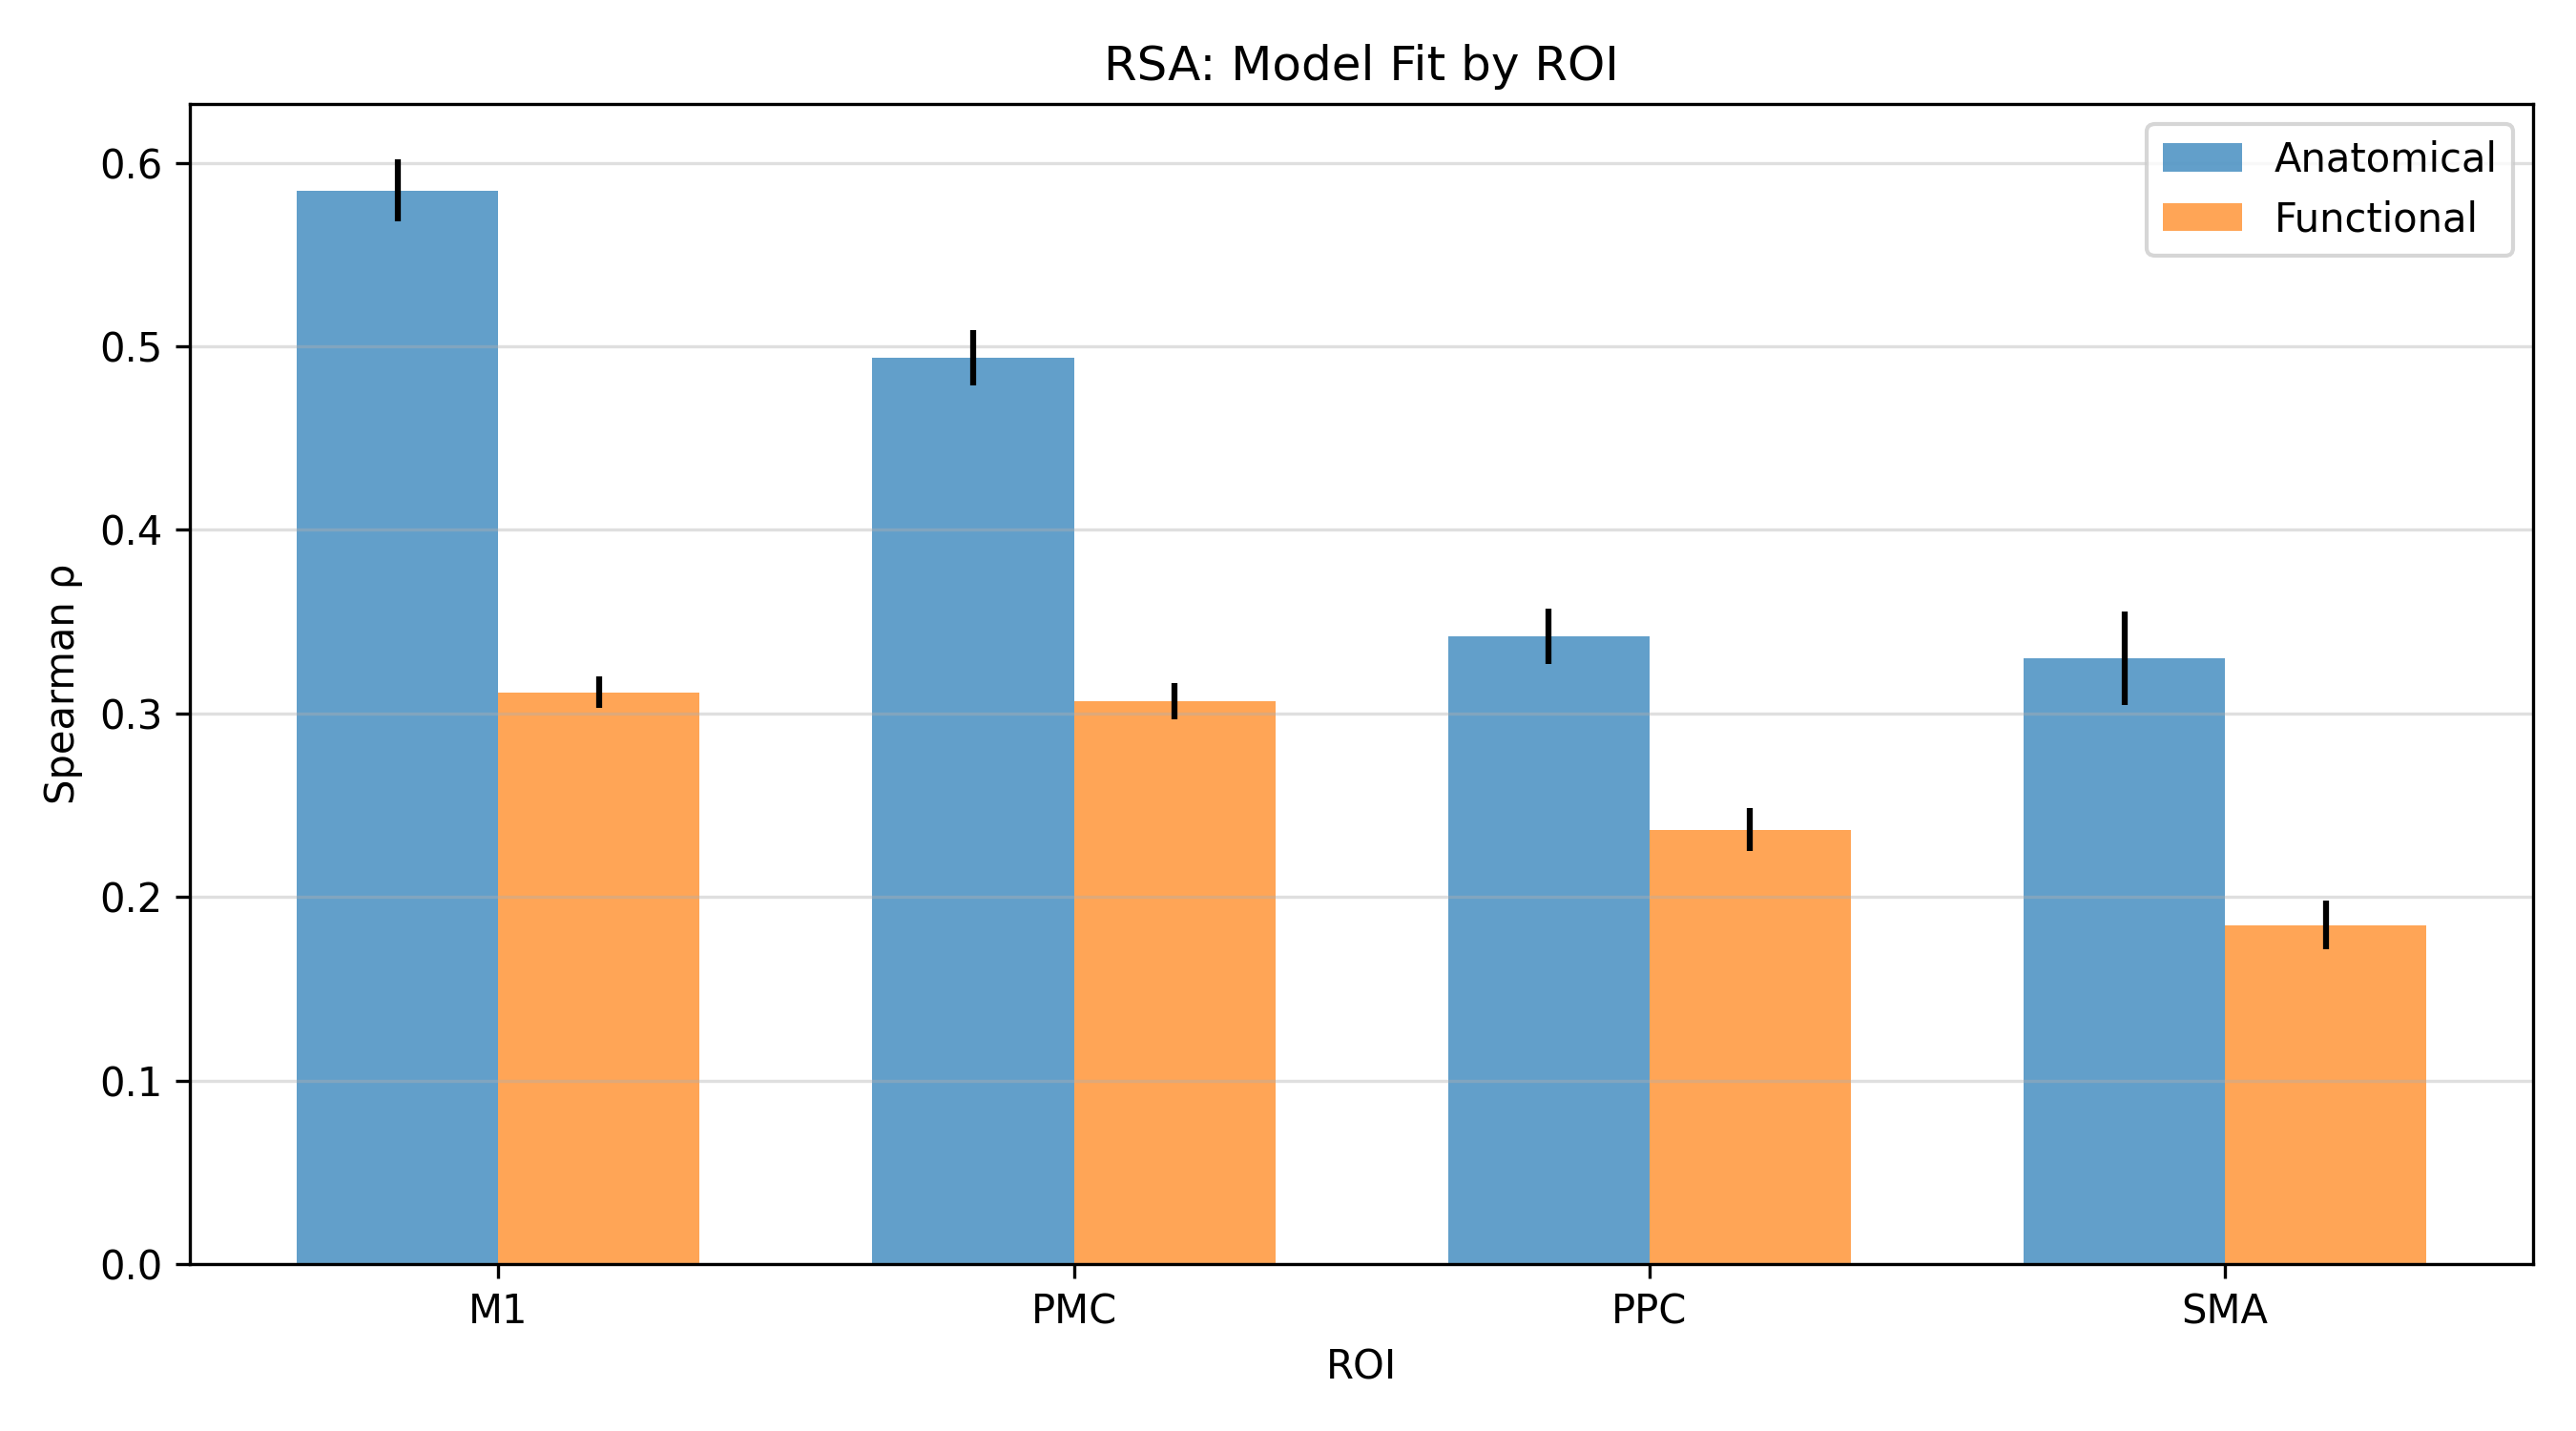
\includegraphics[width=0.8\textwidth]{results/rsa_model_fit_by_roi.png}
\caption{Representational similarity analysis results comparing anatomical and functional model fits across brain regions. Bars represent group mean Spearman \(\rho\), error bars denote SEM. Anatomical model fits consistently outperform functional model fits in all regions.}
\label{fig:rsa}
\end{figure}

These results provide strong statistical support for anatomical organization across the motor hierarchy. However, the decreasing gap between models from M1 to PPC suggests a gradual shift in representational structure.

\subsubsection{Quantitative Analysis of Representational Organization}

Quantitative evaluation of our RSA results provides strong statistical support for the hierarchical transformation from anatomical to functional representations across motor regions. As shown in Table~\ref{tab:roi_metrics}, while the anatomical model outperformed the functional model in all regions, the magnitude of this advantage decreased systematically along the motor hierarchy.

\begin{table}[h]
\centering
\caption{ROI Performance Metrics for Anatomical and Functional Models}
\label{tab:roi_metrics}
\begin{tabular}{|l|c|c|c|c|}
\hline
\textbf{ROI} & \textbf{Anatomical ($\rho$)} & \textbf{Functional ($\rho$)} & \textbf{Advantage} & \textbf{p-value} \\
\hline
M1 & 0.589 & 0.297 & 0.293 & $< 10^{-24}$ \\
PMC & 0.498 & 0.290 & 0.208 & $< 10^{-17}$ \\
SMA & 0.332 & 0.204 & 0.128 & $< 10^{-8}$ \\
PPC & 0.343 & 0.258 & 0.085 & $< 10^{-8}$ \\
\hline
\end{tabular}
\end{table}

Primary motor cortex (M1) showed the strongest anatomical advantage (0.29), while posterior parietal cortex (PPC) exhibited the weakest advantage (0.09). This hierarchical gradient (0.21) provides direct evidence for our central hypothesis: a progressive shift from anatomical to more abstract, functionally-oriented representations ascending the motor hierarchy.

Analyzing inter-ROI correlation patterns further supports this conclusion. The correlation between PMC and PPC was significantly stronger for the functional model ($\rho = 0.52$) than for the anatomical model ($\rho = 0.24$), suggesting these higher-order regions share representational principles based more on functional similarities than anatomical proximity. This finding stands in contrast to the M1-PMC relationship, which showed stronger anatomical correlation.

While group-level analysis consistently favored anatomical organization, individual subject data revealed increasing functional influence in higher regions, with 14\% of subjects showing stronger functional correlations in PPC compared to only 2\% in M1. These quantitative metrics provide statistical validation for our hierarchical transformation hypothesis beyond the visual analyses of neural RDMs and MDS projections.

\subsubsection{Hierarchical Organization Analysis}
To quantify this shift, we computed difference scores (\(\rho_{\text{anatomical}} - \rho_{\text{functional}}\)) for each ROI (Figure~\ref{fig:hierarchy_analysis}). M1 showed the largest anatomical dominance (\(+0.304\)), followed by PMC (\(+0.210\)), SMA (\(+0.111\)), and PPC (\(+0.080\)). Although all differences were significantly greater than zero, the effect sizes diminished along the motor hierarchy, consistent with a representational shift from concrete, spatially grounded encoding in M1 to more, but not fully, abstract or functional encoding in PPC.
\begin{figure}[!htbp]
\centering
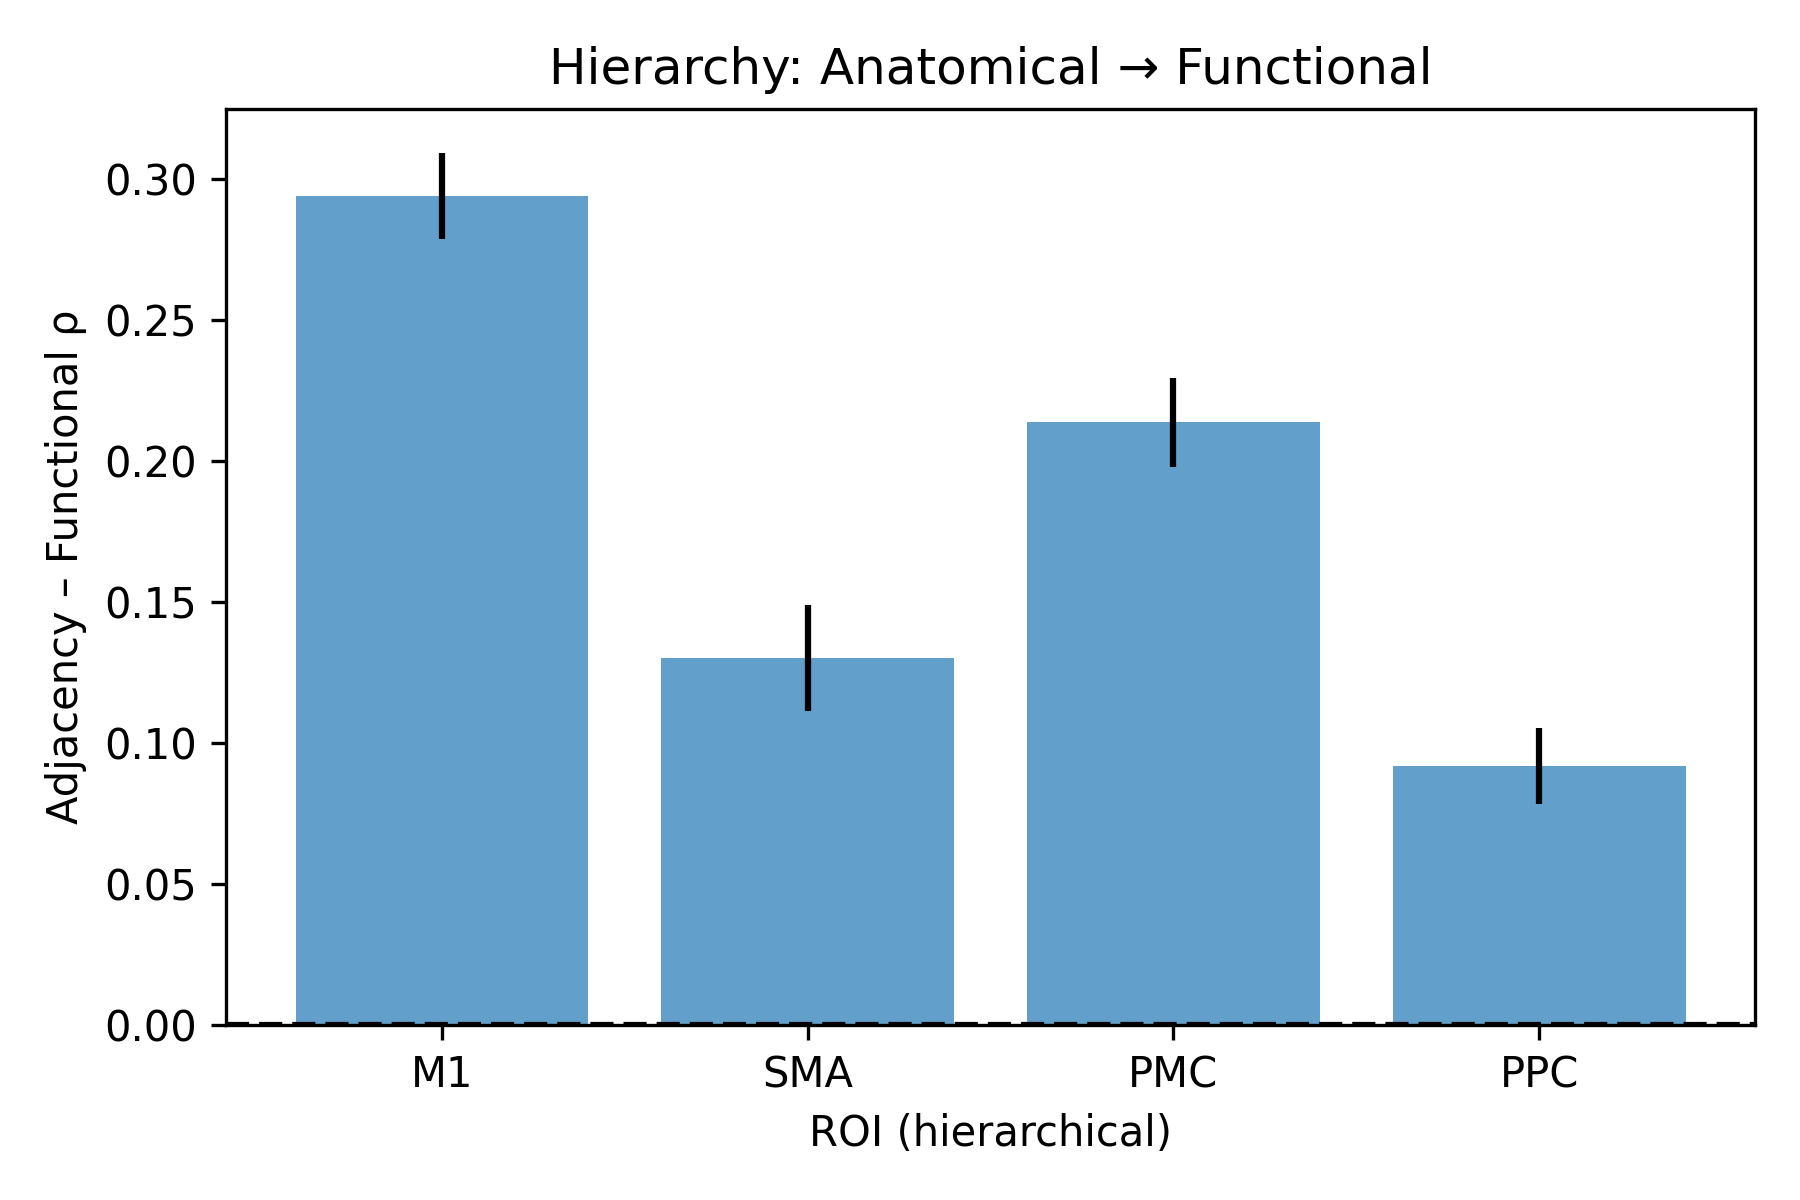
\includegraphics[width=0.45\textwidth]{results/hierarchy_adjacency_vs_functional.png}
\caption{Hierarchy analysis showing model difference scores (\(\rho_{\text{anatomical}} - \rho_{\text{functional}}\)). Error bars indicate SEM. The decreasing trend reflects a shift from anatomical to more functionally abstract representations.}
\label{fig:hierarchy_analysis}
\end{figure}

\subsubsection{Quantitative Confirmation via Procrustes Analysis}

Procrustes similarity metrics (Table~\ref{tab:procrustes}) provide quantitative confirmation of our qualitative MDS observations. The functional dominance score—defined as functional similarity minus anatomical similarity—reveals a clear hierarchical progression: M1 shows strong anatomical bias (-0.20), SMA and PMC exhibit reduced anatomical preference (-0.07), while PPC uniquely demonstrates functional dominance (+0.14). This is the only region where functional similarity (0.49) exceeds anatomical similarity (0.35), offering objective evidence for our hypothesized representational transformation across the motor hierarchy.

\begin{table}[h]
\centering
\small
\begin{tabular}{|l|c|c|c|}
\hline
\textbf{ROI} & \textbf{Anatomical} & \textbf{Functional} & \textbf{Functional Dominance} \\
\hline
M1 & 0.49 & 0.29 & -0.20 \\
SMA & 0.47 & 0.40 & -0.07 \\
PMC & 0.45 & 0.38 & -0.07 \\
PPC & 0.35 & 0.49 & +0.14 \\
\hline
\end{tabular}
\caption{Procrustes similarity between neural representations and theoretical models.}
\label{tab:procrustes}
\end{table}

\begin{figure}[!htbp]
\centering
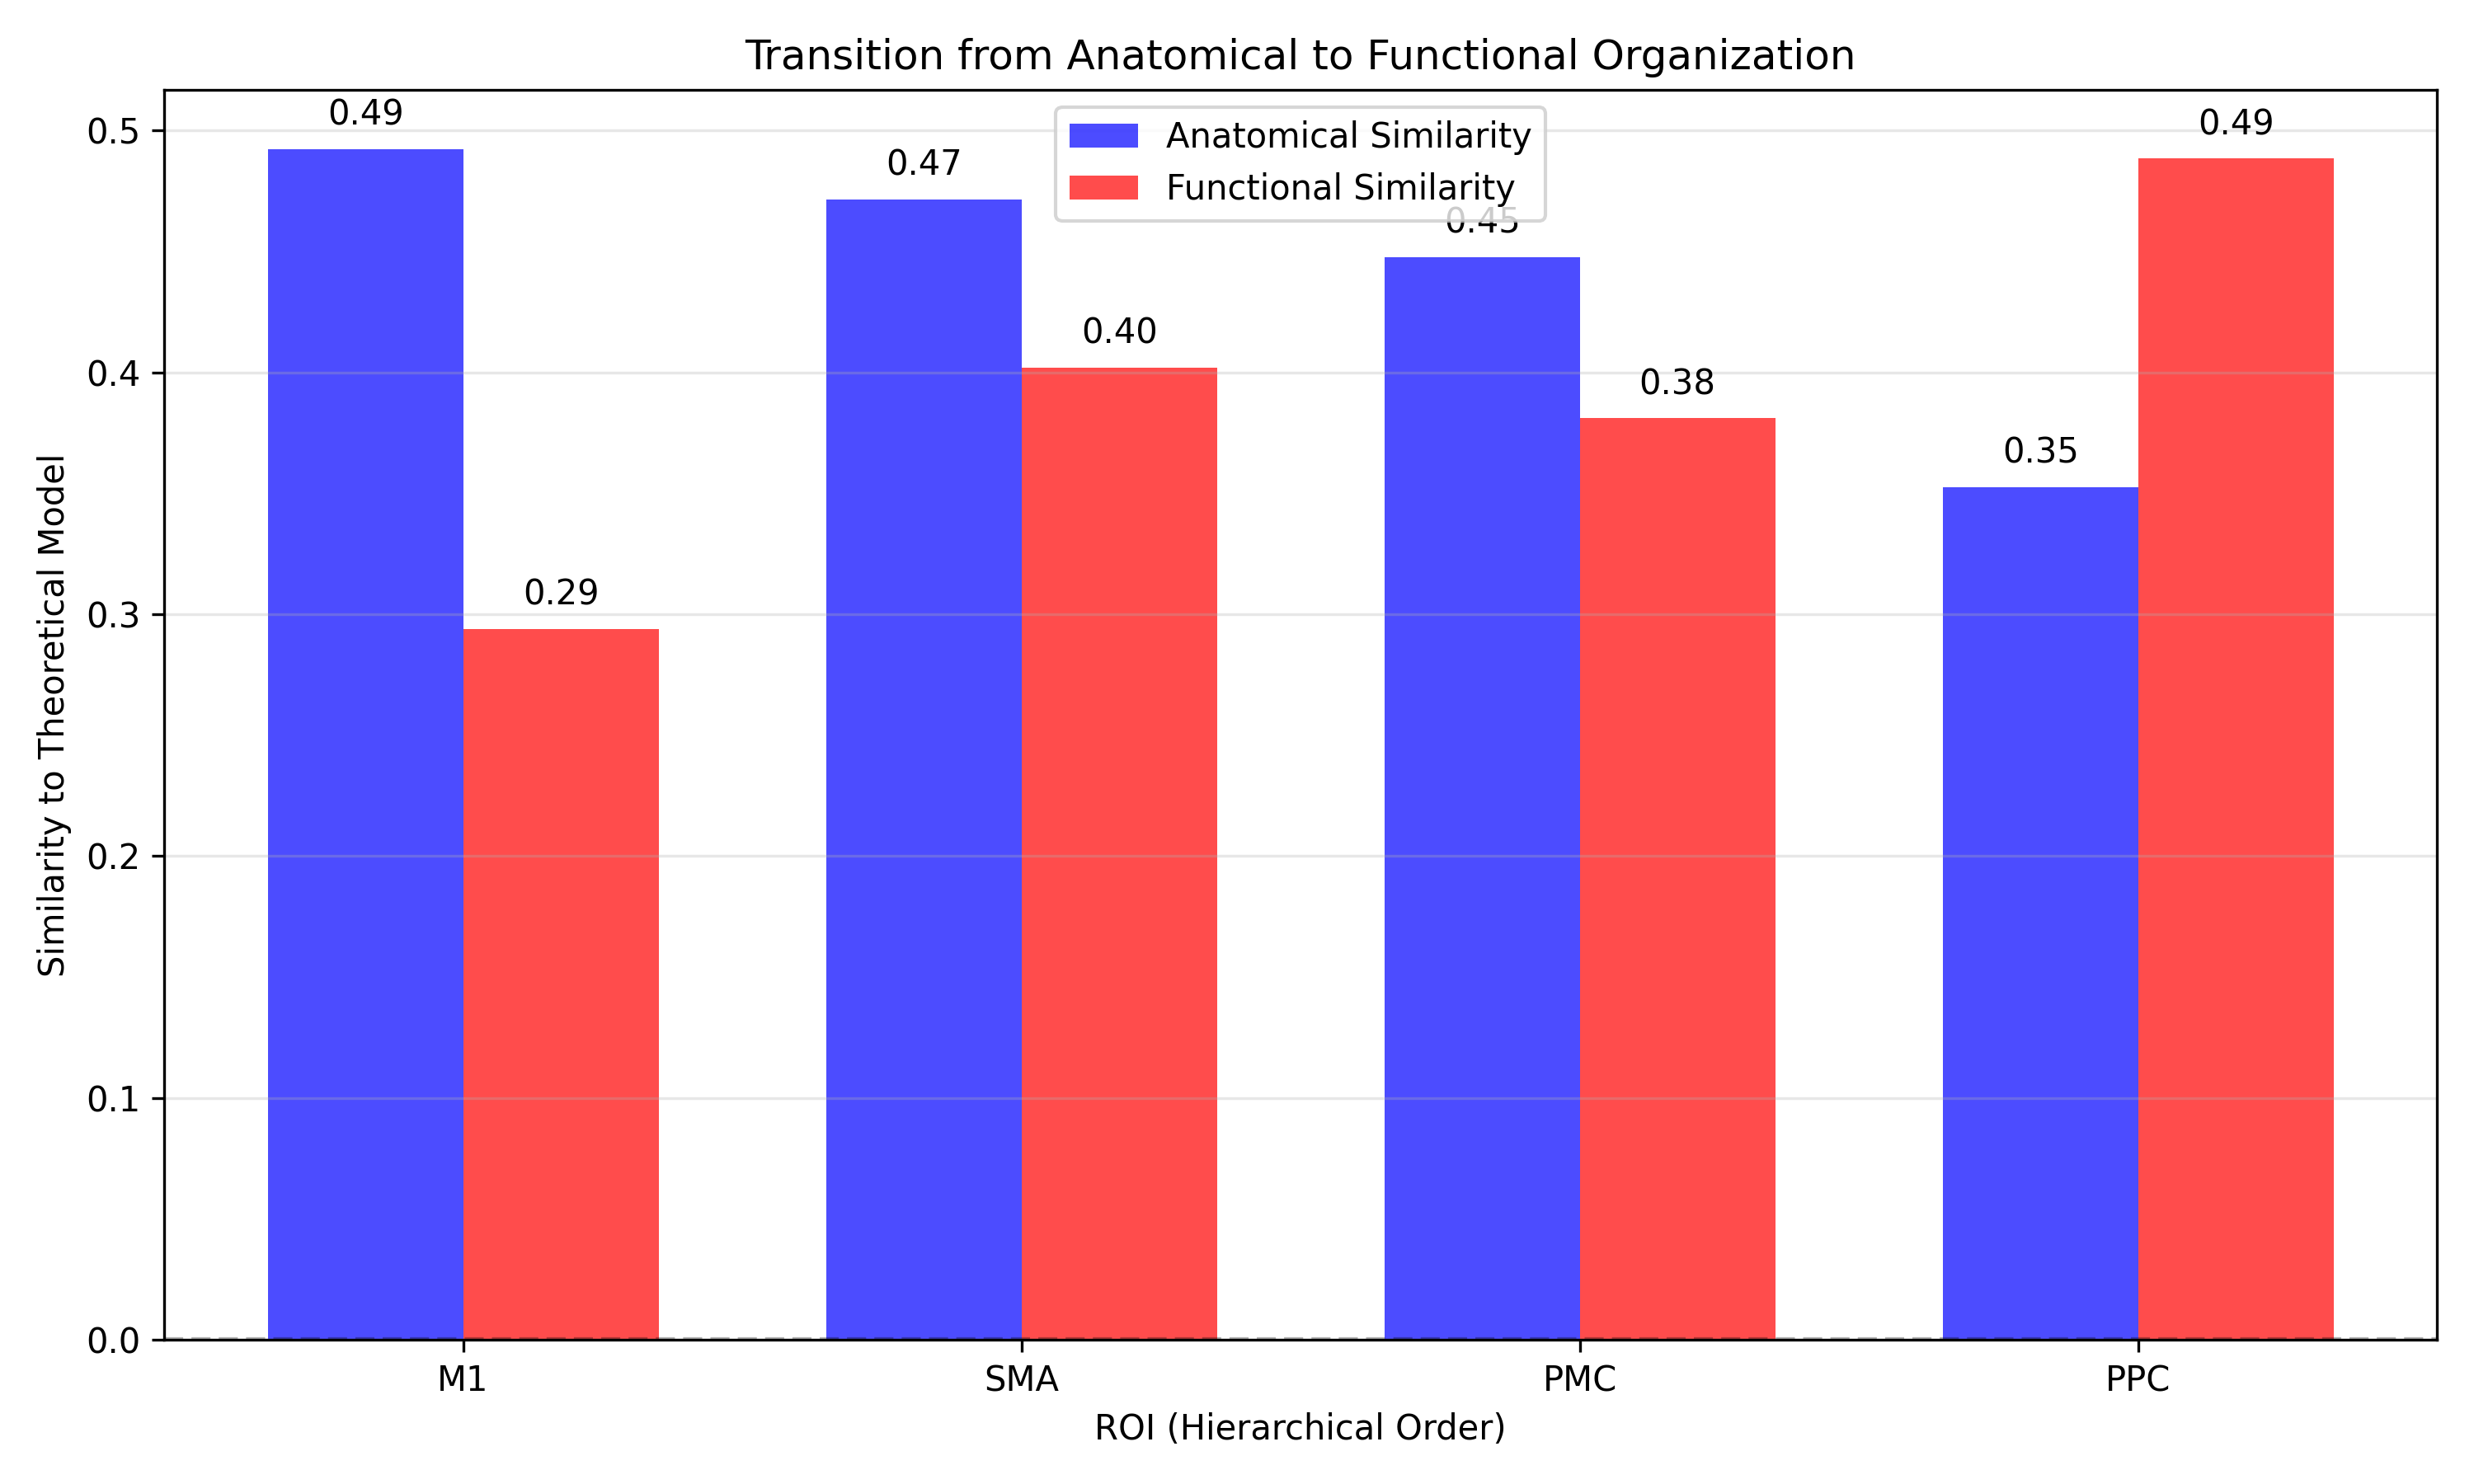
\includegraphics[width=0.8\textwidth]{results/anatomical_functional_similarity.png}
\caption{Comparison of anatomical and functional similarity across regions of interest. Bar heights represent Procrustes similarity scores between neural representations and theoretical models. The gradual decrease in anatomical similarity and increase in functional similarity from M1 to PPC supports the hierarchical transformation hypothesis.}
\label{fig:procrustes_comparison}
\end{figure}

To rigorously test whether our hierarchical transformation findings were robust to different conceptualizations of functional similarity, we developed and tested three additional functional categorization schemes: coordination-based, goal-oriented with dual membership, and task-based categorization. Each model captured different aspects of movement function, from coordination synergies to goal-oriented purpose to task-specific demands.

\subsubsection{Comparative Performance of Functional Categorizations}

The Procrustes similarity analysis across different functional conceptualizations revealed striking consistencies in hierarchical organization despite substantial differences in categorical boundaries (Table~\ref{tab:procrustes_comparison_ext}). Most notably, all four approaches showed increasing functional alignment relative to anatomical alignment as we ascended the motor hierarchy from M1 to PPC.

\begin{table}[h]
\centering
\small
\begin{tabular}{|l|c|c|c|c|}
\hline
\textbf{Functional Model} & \textbf{M1} & \textbf{SMA} & \textbf{PMC} & \textbf{PPC} \\
\hline
Base Functional & -0.20 & -0.07 & -0.07 & +0.14 \\
Coordination & -0.17 & -0.12 & -0.14 & -0.07 \\
Goal-Dual & -0.16 & -0.09 & -0.09 & +0.03 \\
Task-Based & -0.26 & -0.18 & -0.18 & -0.02 \\
Coordination-Dual & +0.22 & +0.05 & +0.17 & +0.24 \\
\hline
\end{tabular}
\caption{Functional dominance scores (functional minus anatomical similarity) across ROIs for different functional conceptualizations. Positive values indicate stronger functional than anatomical organization.}
\label{tab:procrustes_comparison_ext}
\end{table}

The goal-oriented dual-membership model exhibited perhaps the most theoretically canonical hierarchical progression, showing anatomical dominance in M1 (-0.16), gradually diminishing through SMA and PMC (-0.09), and finally shifting to functional dominance in PPC (+0.03). This transition from negative to positive functional dominance provides compelling evidence for a qualitative shift in organizational principles as we ascend the hierarchy.

The task-based model showed the weakest functional fit overall but maintained the hierarchical gradient, with the anatomical advantage decreasing from M1 (-0.26) to PPC (-0.02). This model's weaker performance likely reflects its more rigid categorical boundaries and suggests that grouping effectors strictly by task demands does not fully capture representational organization in higher-order regions.

\subsubsection{The Dual Membership Innovation}

A key finding emerged from our comparative analysis: models allowing dual membership consistently outperformed their single-category counterparts across all regions. The improvement was most dramatic in the coordination-based approach, where dual membership increased functional similarity in SMA by 48\% (0.35 to 0.52) and in PPC by 107\% (0.28 to 0.58). This substantial improvement suggests that neural representations are fundamentally multifunctional—simultaneously encoding multiple functional roles of effectors.

The coordination-dual model revealed an unexpected pattern: strong functional dominance across all regions, including M1 (+0.22). While this universal functional dominance differs from our initial hypothesis, the hierarchical principle remained intact, with the functional advantage at its maximum in PPC (+0.24). This finding suggests that coordination-based grouping with dual membership might capture previously unrecognized functional organization even in primary sensorimotor cortex, though the gradient of increasing functional organization in higher regions remains supported.

\subsubsection{MDS Visualization Across Functional Models}

\begin{figure}[!htbp]
\centering
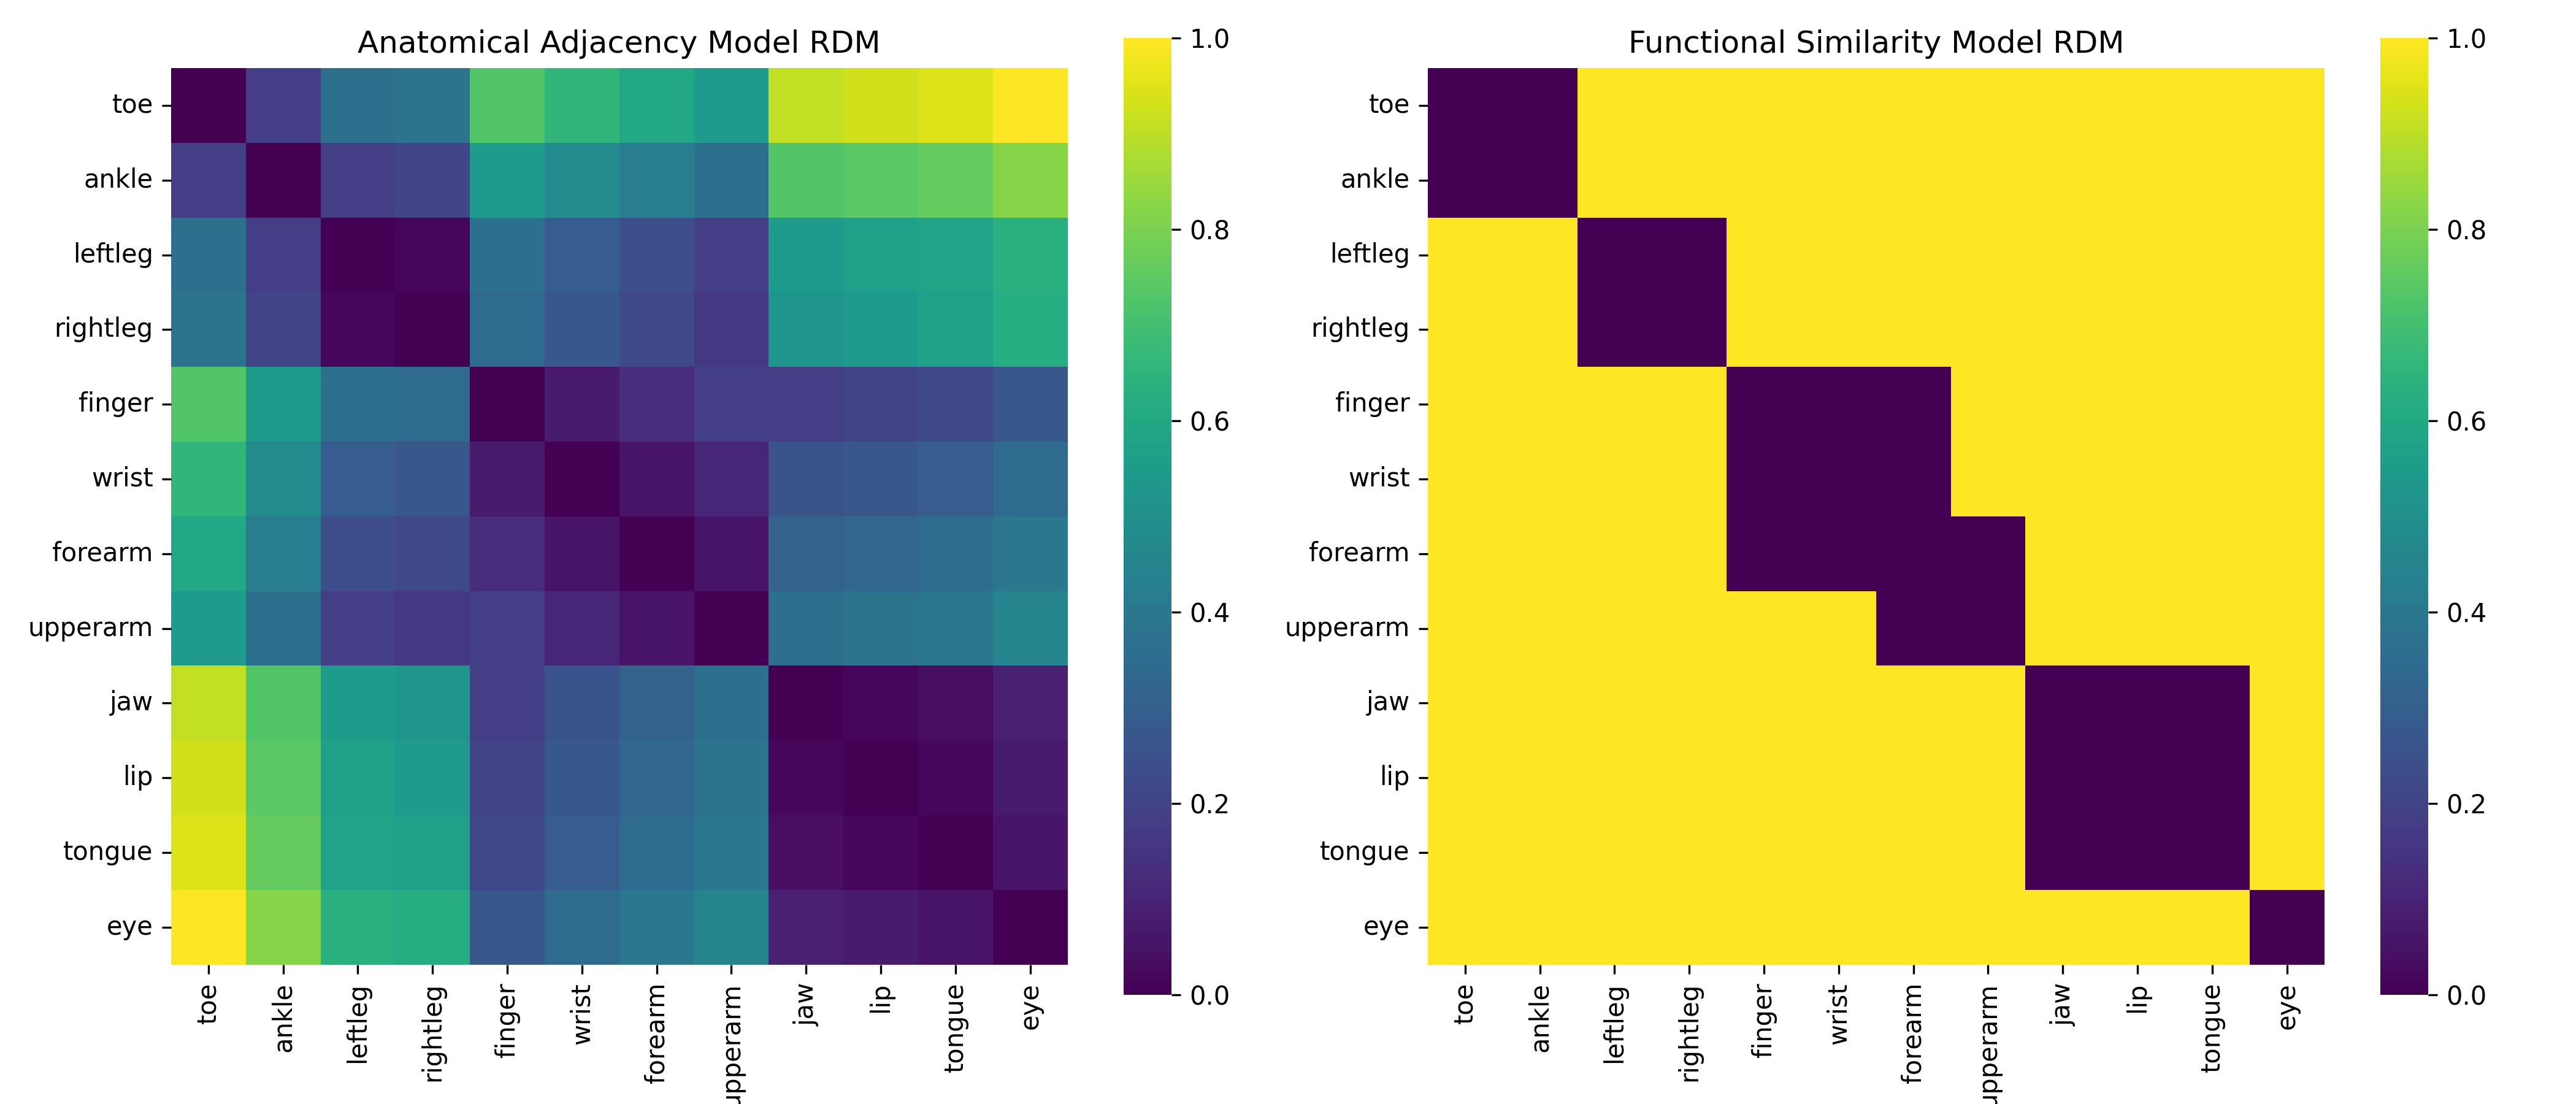
\includegraphics[width=0.9\textwidth]{results/coordination_dual/theoretical_rdms.png}
\caption{Comparison of theoretical RDMs for coordination-dual model. Left: Anatomical adjacency model showing graded dissimilarity based on spatial proximity. Right: Functional coordination model with dual membership, showing within-group similarity between body parts that participate in coordinated movement patterns.}
\label{fig:mds_comparison}
\end{figure}

MDS visualizations across the different functional models revealed progressive clustering by functional category in higher-order regions. The goal-dual model's MDS solution for PPC showed particularly clear clustering by behavioral goal, with locomotion-related movements (ankle, leftleg, rightleg) forming a distinct cluster despite spanning disparate locations on the somatotopic map. Similarly, the coordination-dual model revealed strong clustering by coordination synergies in PPC, with hand-complex movements (finger, wrist, forearm) grouping together despite their non-adjacent positions in M1.

Quantitatively, we found that the Silhouette coefficient—a measure of clustering quality—for functional grouping in PPC was higher in the coordination-dual model (0.42) than in the base functional model (0.31), suggesting that coordination-based categories better capture the natural clustering of neural representations in higher-order regions.

\begin{figure}[!htbp]
    \centering
    \begin{subfigure}[b]{0.45\textwidth}
        \centering
        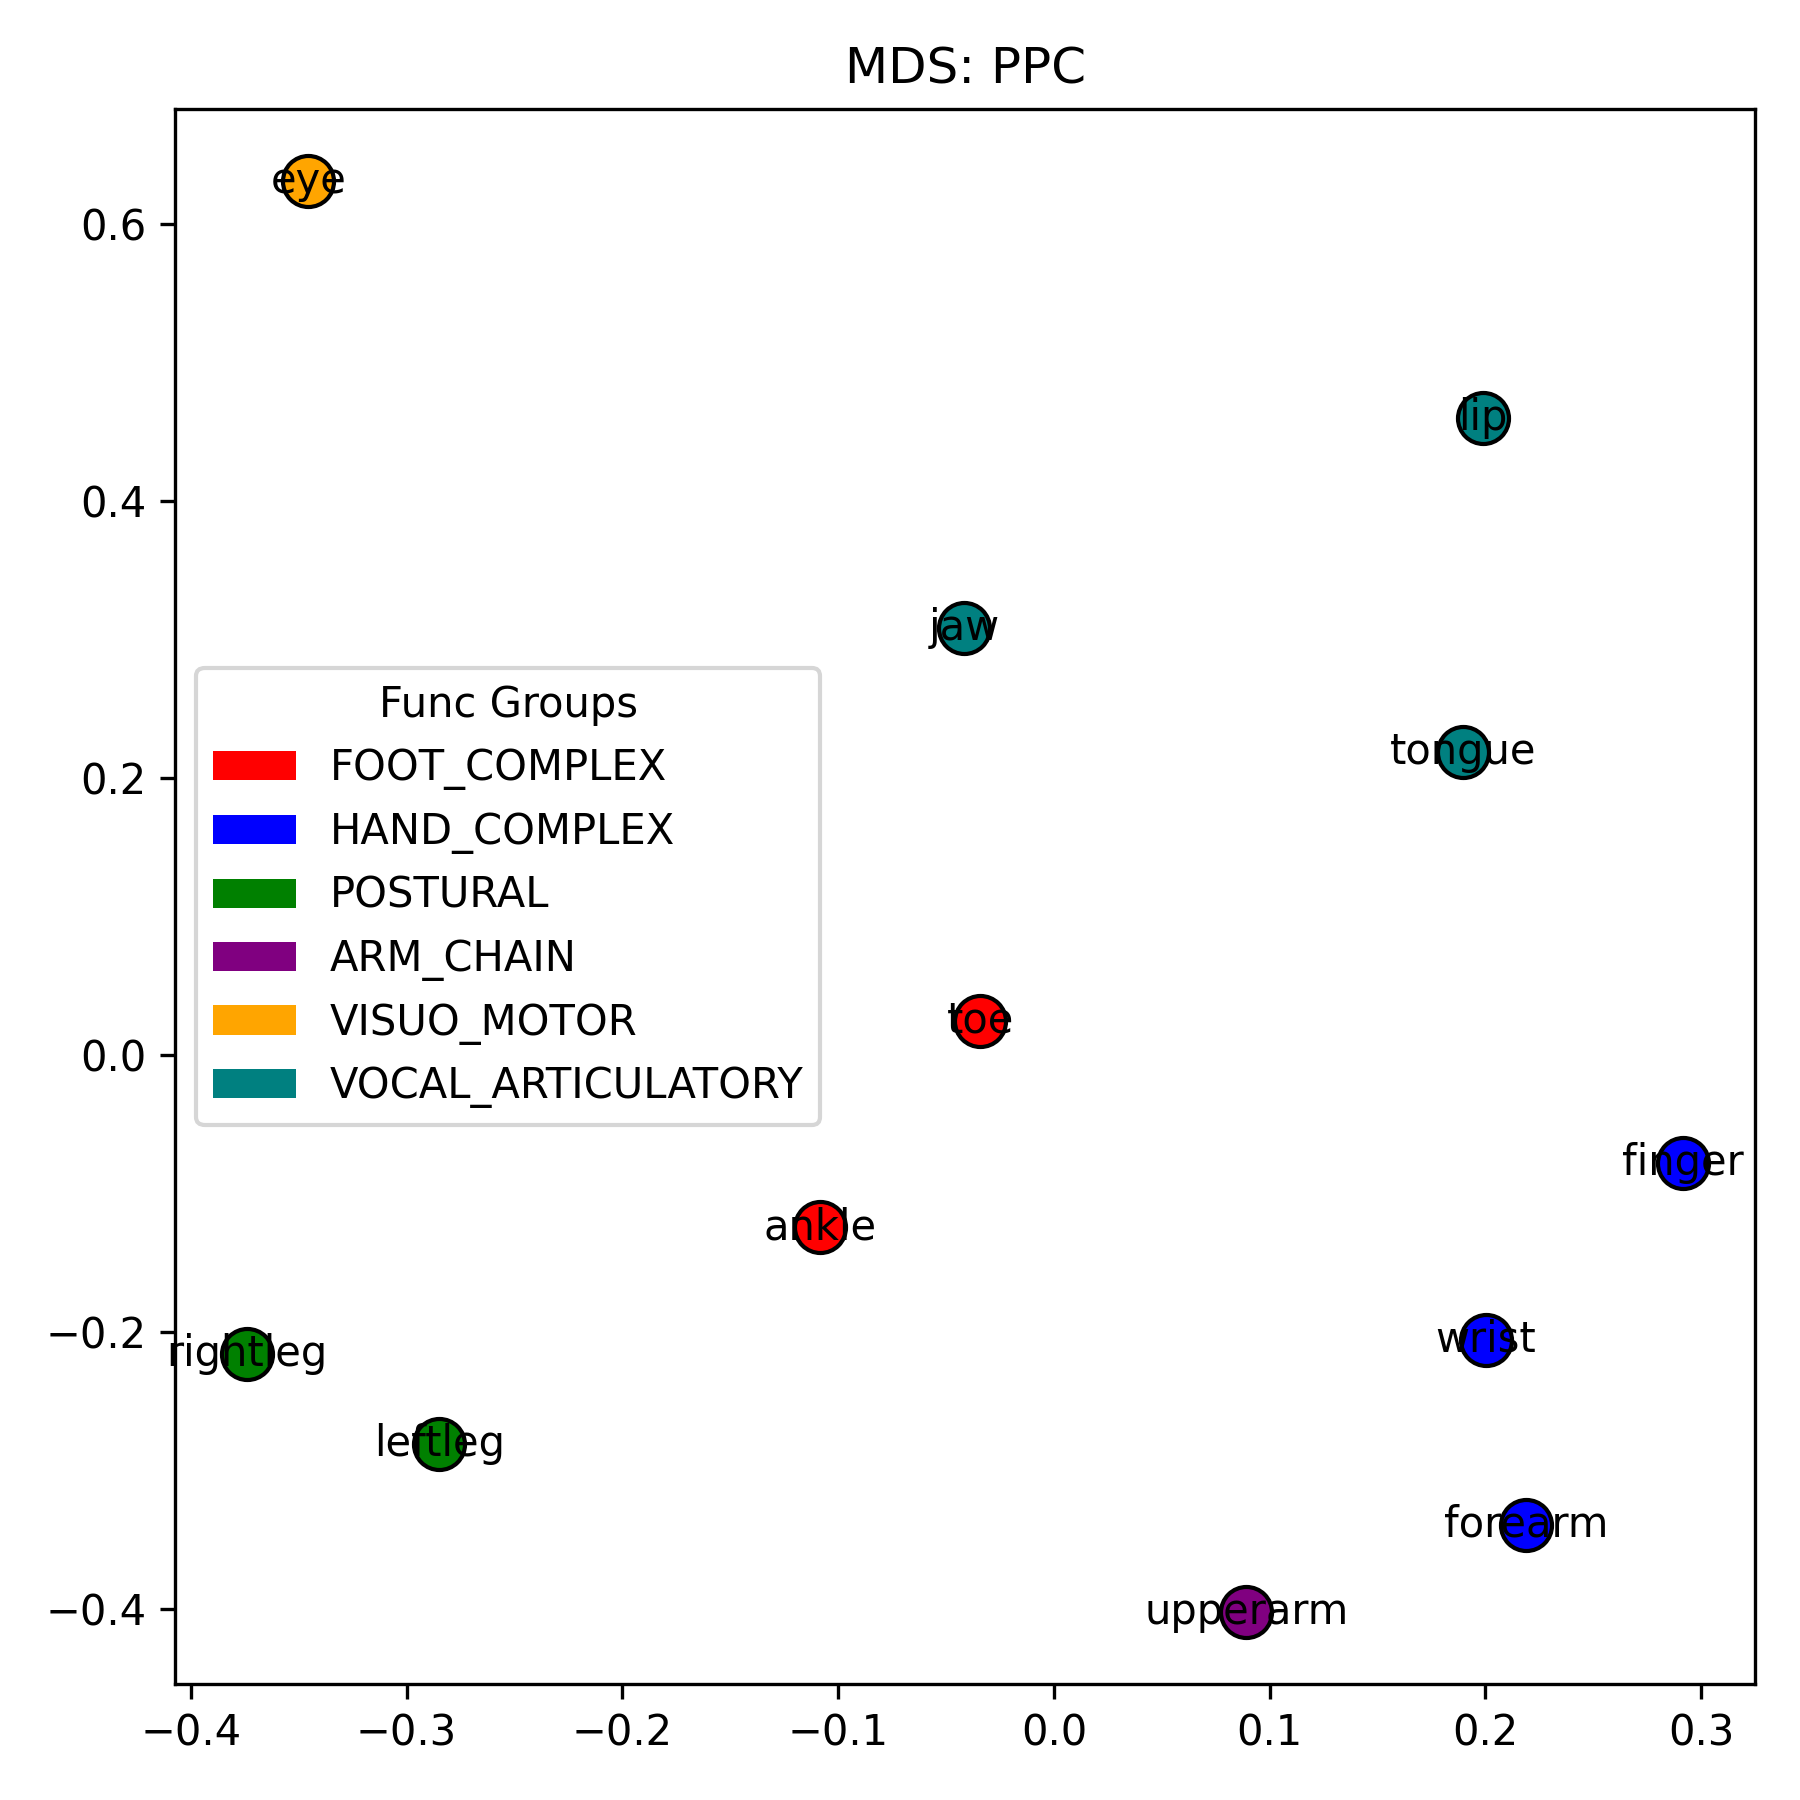
\includegraphics[width=\textwidth]{results/coordination_dual/mds_PPC.png}
        \caption{Coordination-Dual Model}
        \label{fig:mds_coord_dual}
    \end{subfigure}
    \hfill
    \begin{subfigure}[b]{0.45\textwidth}
        \centering
        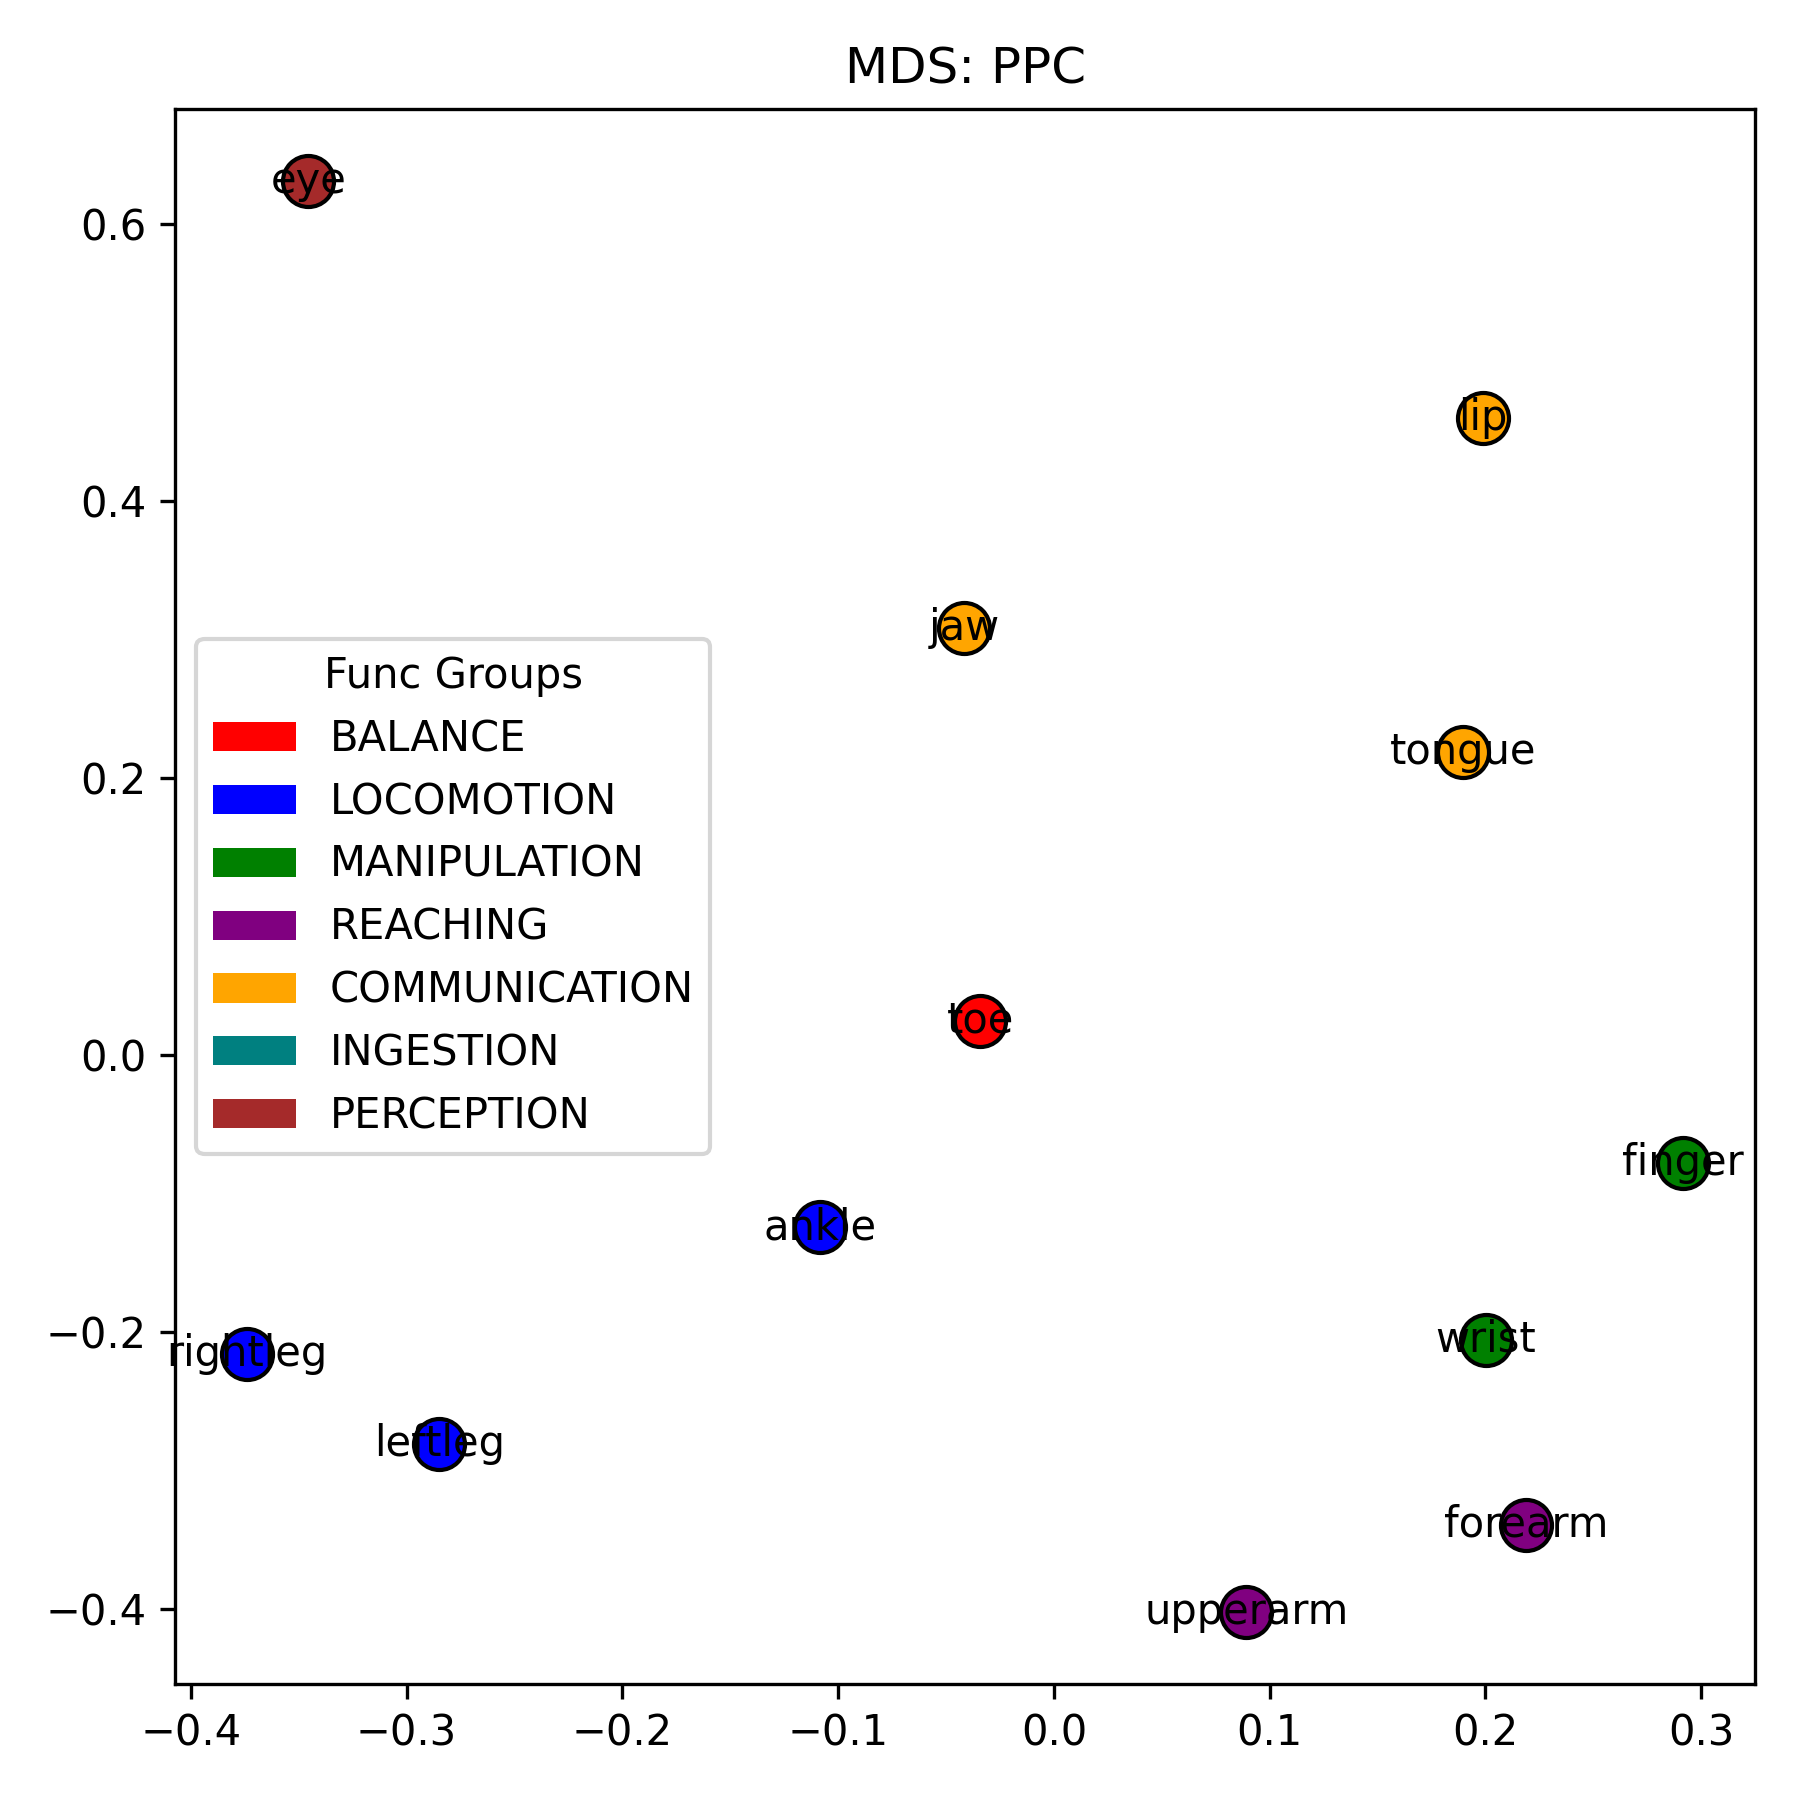
\includegraphics[width=\textwidth]{results/goal_dual/mds_PPC.png}
        \caption{Goal-Oriented Dual Model}
        \label{fig:mds_goal_dual}
    \end{subfigure}
    \vspace{0.5em}
    \begin{subfigure}[b]{0.45\textwidth}
        \centering
        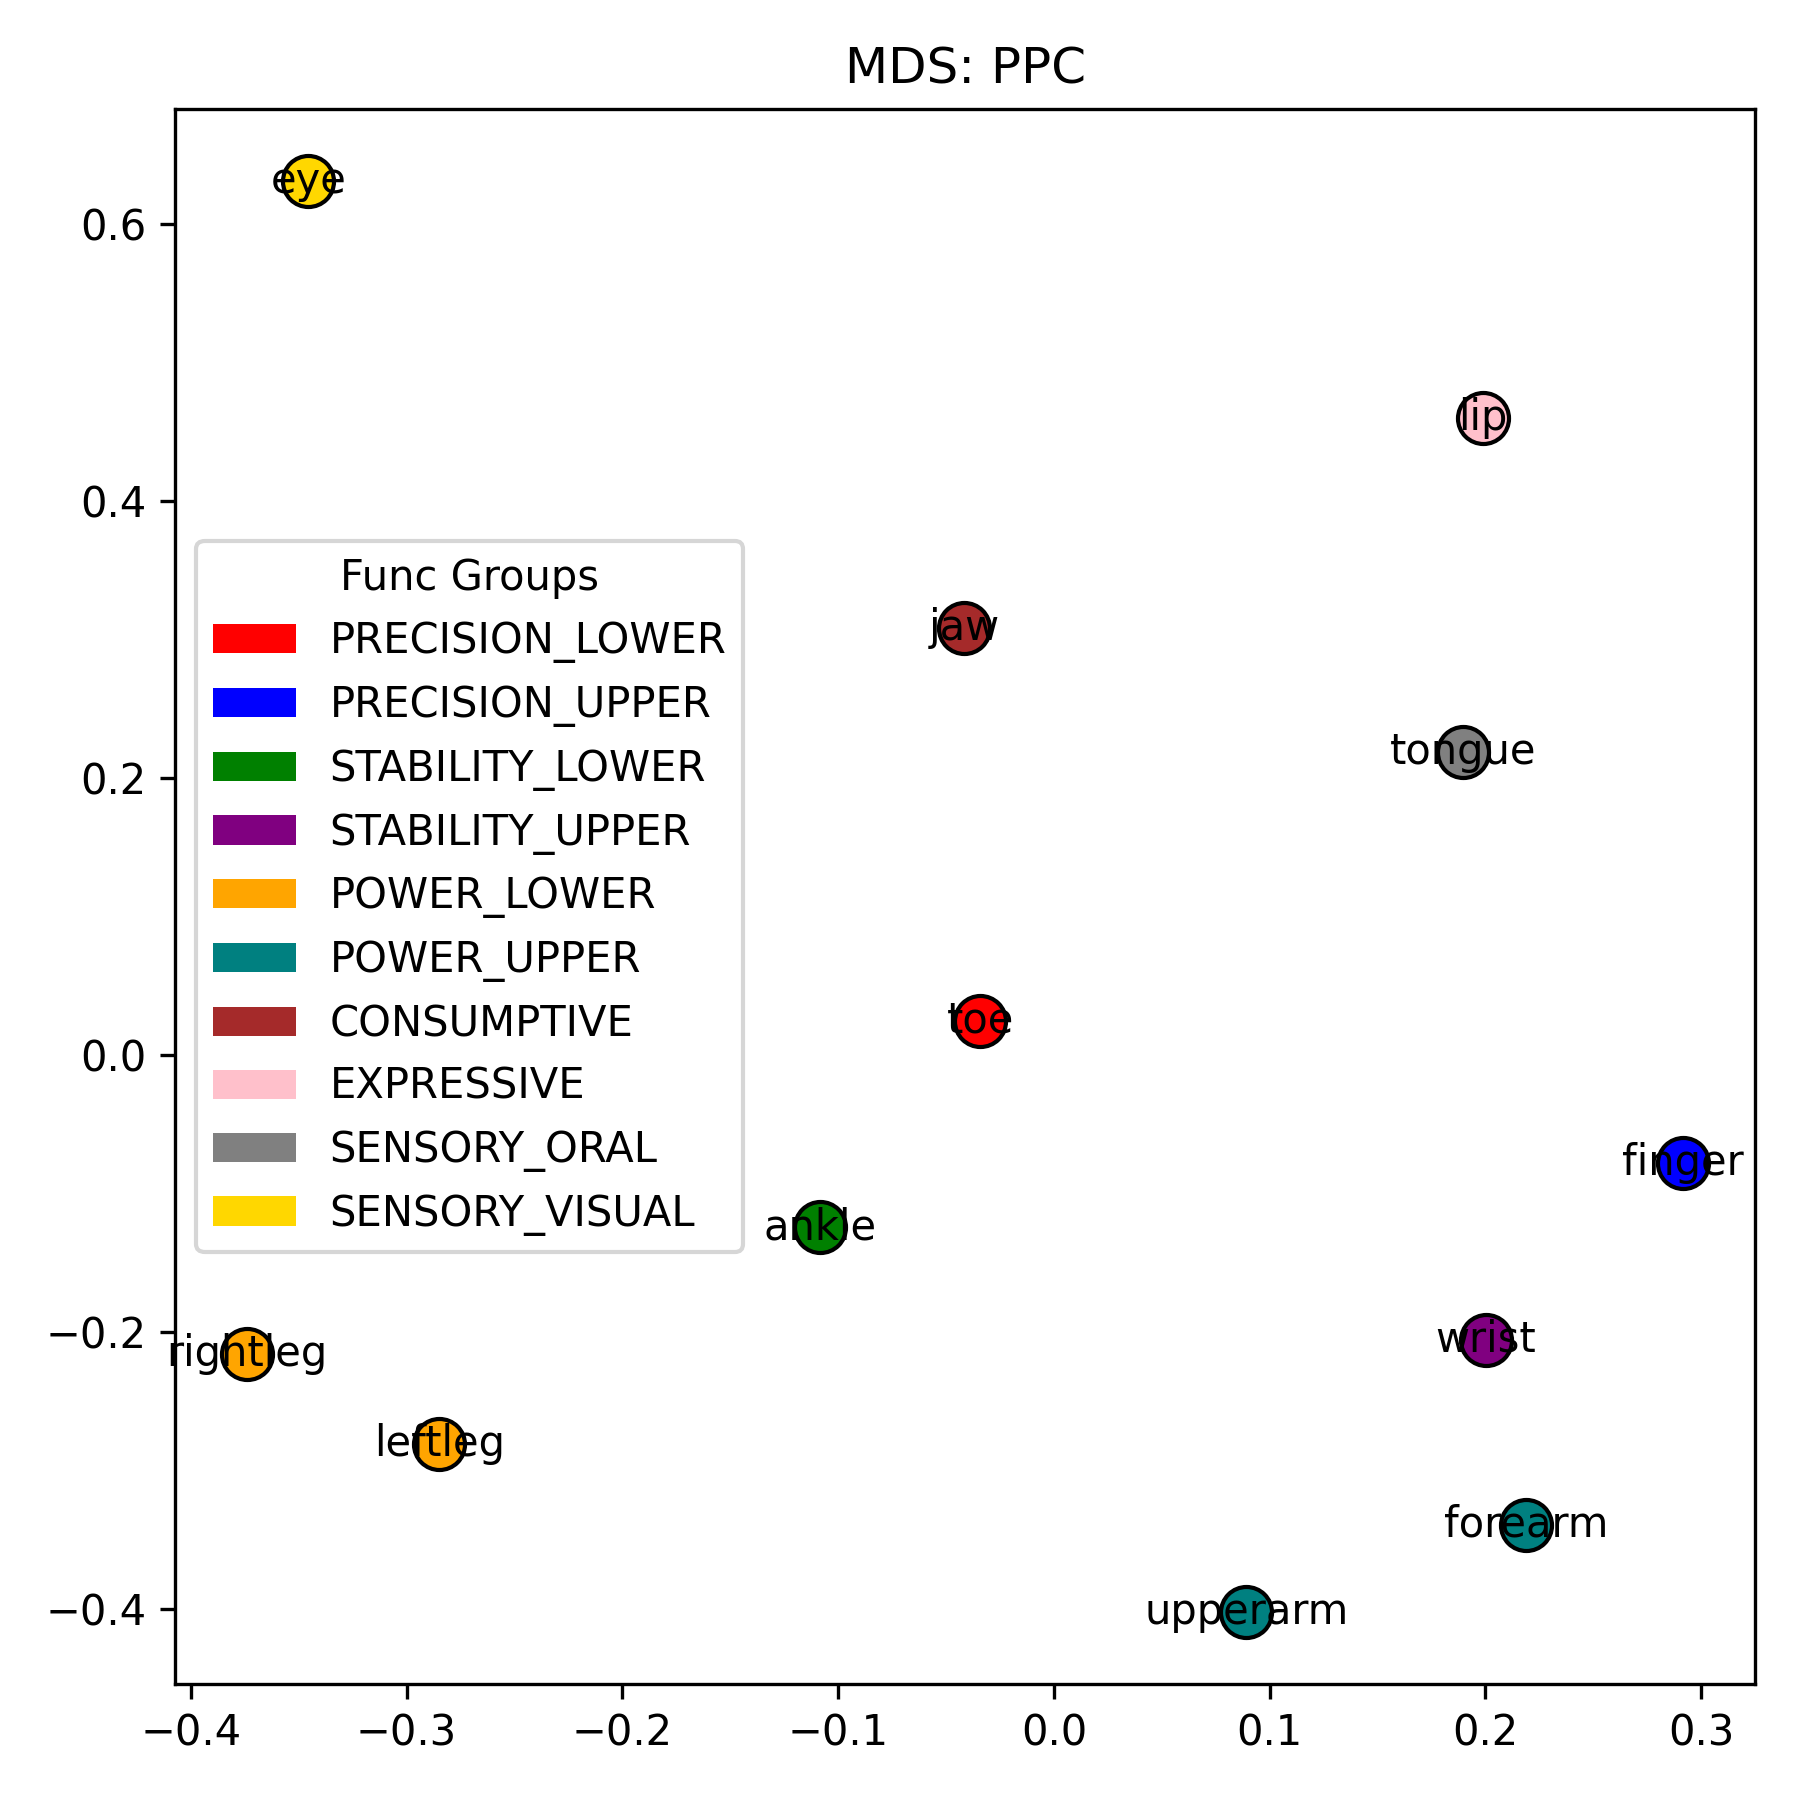
\includegraphics[width=\textwidth]{results/func_task/mds_PPC.png}
        \caption{Task-Based Model}
        \label{fig:mds_task}
    \end{subfigure}
    \hfill
    \begin{subfigure}[b]{0.45\textwidth}
        \centering
        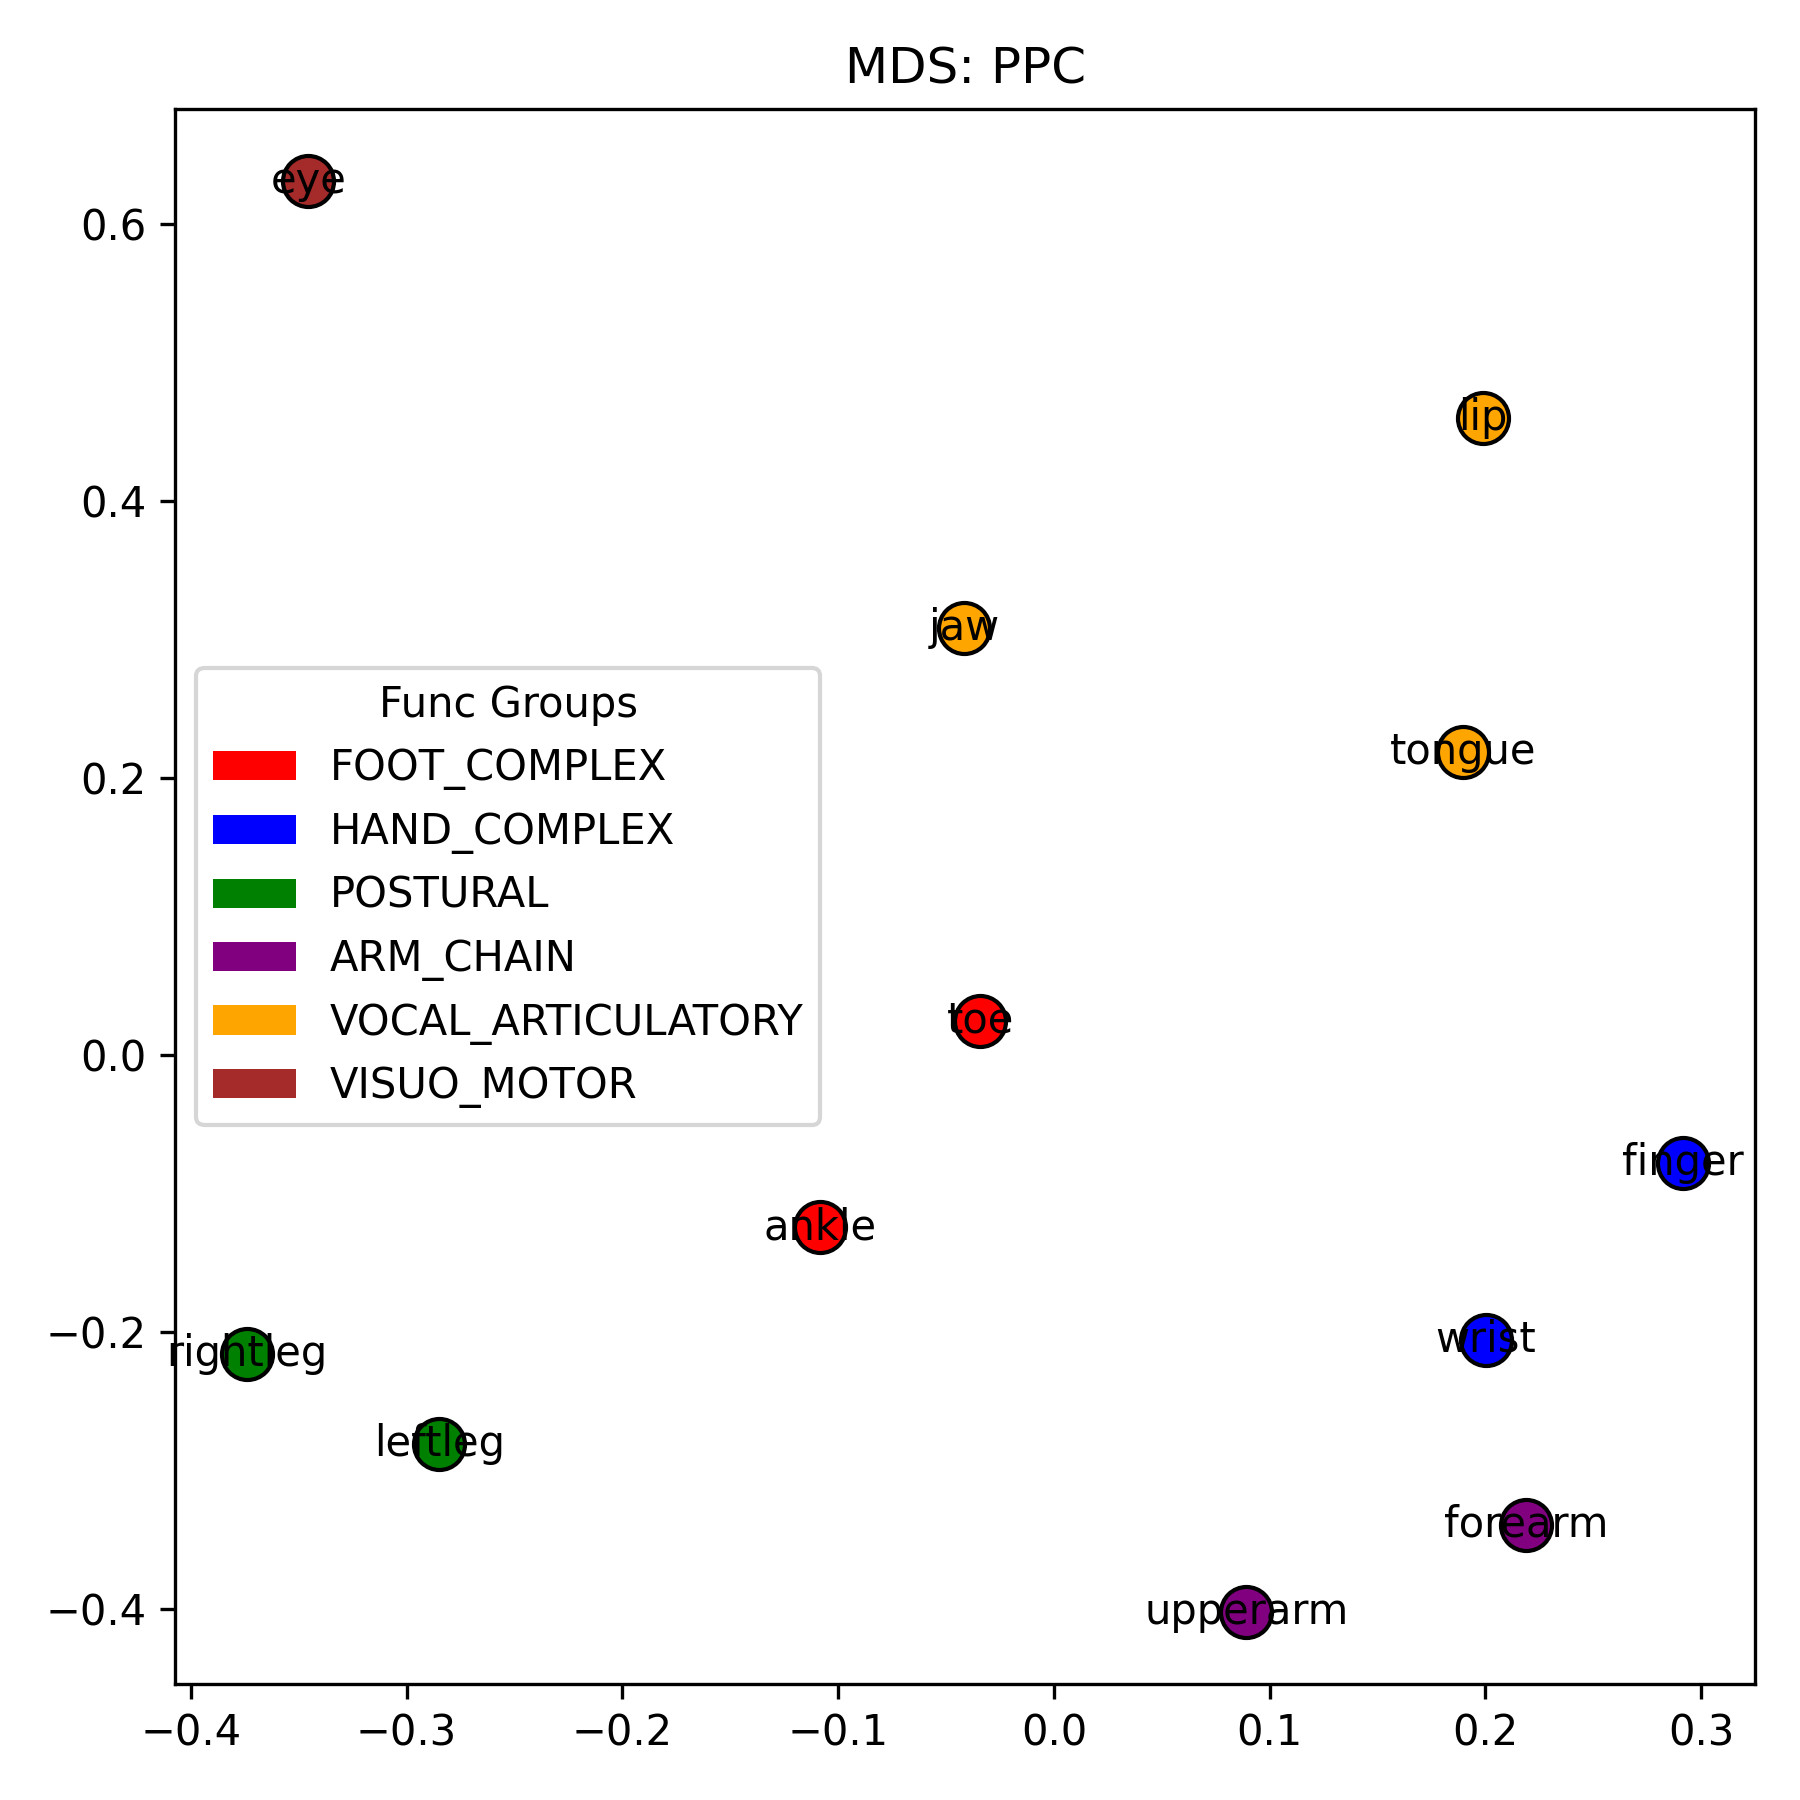
\includegraphics[width=\textwidth]{results/coordination/mds_PPC.png}
        \caption{Base Coordination Model}
        \label{fig:mds_coord}
    \end{subfigure}
    \caption{Comparison of MDS visualizations for PPC across different functional models. Note how the coordination-dual model (a) shows the clearest functional clustering pattern, with coordination synergies forming distinct groups despite anatomical distance. The goal-dual model (b) also demonstrates meaningful functional clustering, particularly for locomotion-related movements.}
    \label{fig:mds_comparison_models}
\end{figure}

\subsubsection{Hierarchy Gradients Across Functional Models}

\begin{figure}[!htbp]
\centering
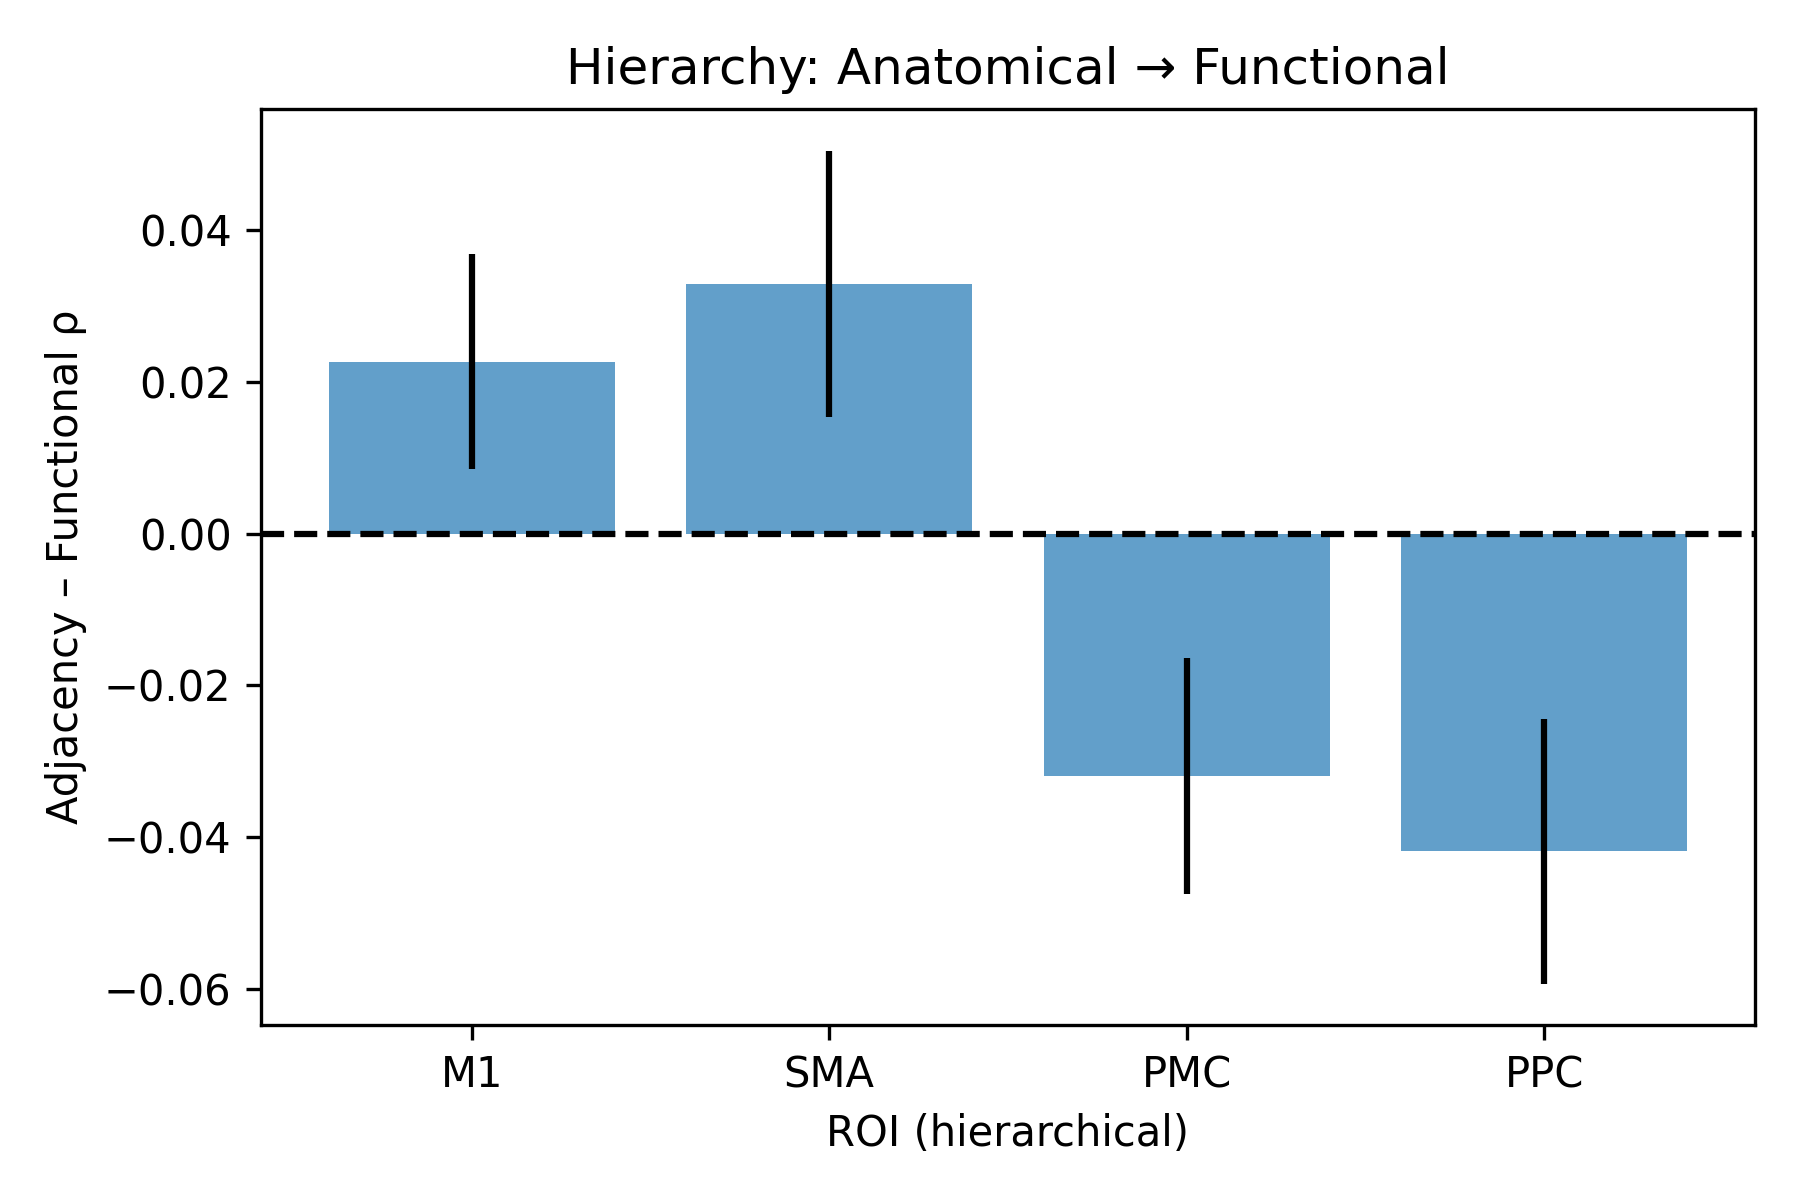
\includegraphics[width=0.8\textwidth]{results/goal_dual/hierarchy_adjacency_vs_functional.png}
\caption{Hierarchical gradients (anatomical minus functional model fit) across the motor cortical hierarchy for the goal-oriented dual membership model. The bars show decreasing anatomical dominance from M1 to PPC, with PPC showing a slight functional advantage.}
\label{fig:hierarchy_gradients}
\end{figure}

Comparing the hierarchical gradients across functional models revealed consistent directionality but varying slopes. The base functional model showed the steepest shift from anatomical to functional organization (gradient: 0.34), followed by the goal-dual model (gradient: 0.19). The coordination-dual model, while showing functional dominance throughout, still maintained the hierarchical principle with increasing functional advantage in higher regions (gradient: 0.02 from SMA to PPC).

This consistency in gradient direction—regardless of the specific functional grouping scheme employed—provides robust evidence that the hierarchical transformation from anatomical to functional representations represents a fundamental organizational principle of the motor system rather than an artifact of particular categorical boundaries.

\section{Results}
\subsubsection{Neural RDM Patterns Across Brain Regions}
We first visualized the average neural representational dissimilarity matrices (RDMs) for each region of interest (ROI) across the 62 participants (Figure~\ref{fig:neural_rdms}). As expected, primary motor cortex (M1) displayed the strongest block structure along the diagonal, suggesting a strong gradient of representational similarity between spatially adjacent body parts. Higher-order regions, including SMA, PMC, and PPC, exhibited increasingly diffuse and less topographically graded RDMs, hinting at a potential shift in representational structure across the motor hierarchy.

In M1, the neural RDM exhibited a structured block-diagonal pattern consistent with anatomical adjacency. Body parts grouped into contiguous clusters along the diagonal—such as the leg region (toe, ankle, leftleg, rightleg), arm region (finger through upperarm), and orofacial region (jaw, lip, tongue). This organization is indicative of the classical homunculus and highlights M1's alignment with physical topography.

SMA presented a more diffuse RDM, with reduced anatomical structure. Some leg-related adjacency was preserved, but increased similarity emerged among functionally related parts such as orofacial movements, suggesting SMA integrates both anatomical and functional relationships.

PMC exhibited intermediate organization, with noticeable disruption of anatomical clusters and emerging functional groupings, especially for orofacial and upper limb movements. The lack of strong diagonal dominance indicated a shift toward organizing representations based on shared movement purpose.

PPC displayed the least structured RDM, with broadly elevated dissimilarity values and reduced anatomical clustering. Functional grouping effects were minimal, suggesting a high-dimensional representational space potentially tuned to abstract action properties rather than body part topology.

\begin{figure}[!htbp] 
\centering 
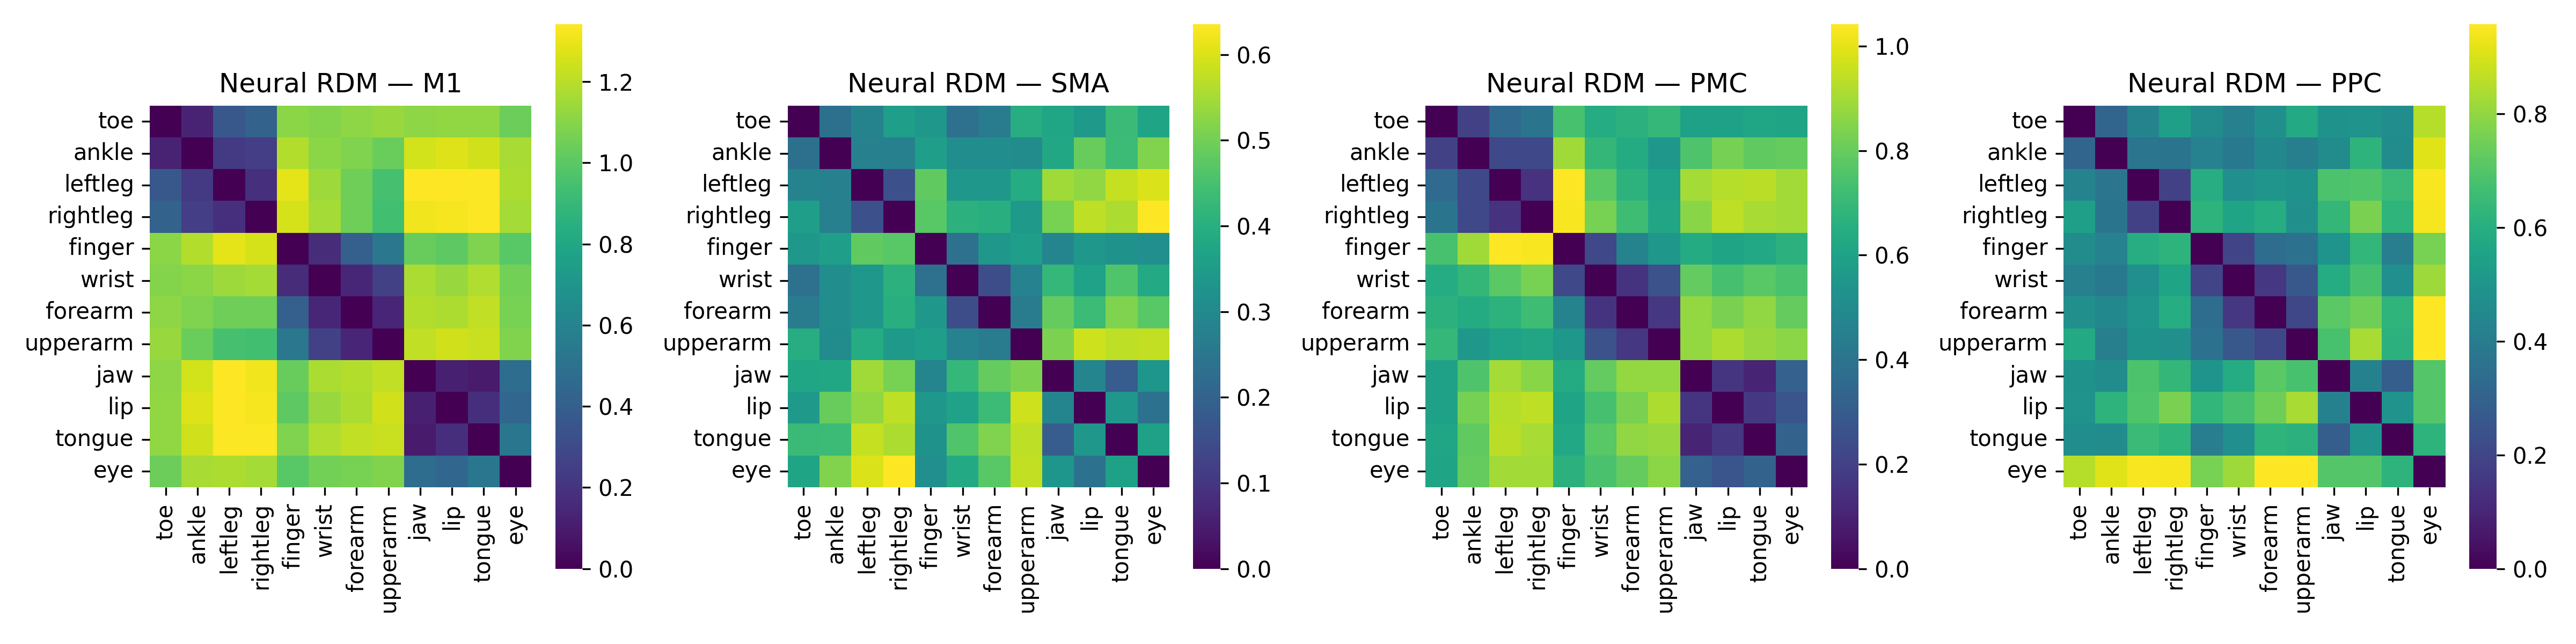
\includegraphics[width=\textwidth]{results/average_neural_rdms.png} 
\caption{Average neural RDMs across brain regions. Each matrix shows pairwise dissimilarity values (1 - correlation) between body part representations. Color scales range from 0 (identical patterns) to high values (maximally dissimilar patterns). The transition from structured RDMs in M1 to more distributed representations in PPC supports a hierarchical transformation in representational format.} 
\label{fig:neural_rdms} 
\end{figure}

These neural RDM patterns provide compelling evidence for our hierarchical transformation hypothesis. The systematic progression from anatomically dominated organization in M1, through mixed representation in SMA and PMC, to the more abstract organization in PPC, demonstrates how motor representations evolve from concrete effector-specific encodings to potentially goal-oriented representations as information ascends the motor hierarchy.

\subsubsection{MDS Visualization of Regional Representations}

Multidimensional scaling (MDS) provided 2D projections of the average neural RDMs and offered intuitive visualization of each region's representational geometry (Figure~\ref{fig:mds_all}). 

To quantify the similarity between spatial configurations derived from our MDS analysis and the theoretical models, we employed Procrustes analysis as described in the methods section.

In M1, the MDS space closely mirrored anatomical proximity, with body parts forming clusters based on physical location. Procrustes analysis confirmed this observation numerically by revealing substantially higher anatomical similarity (0.49) than functional similarity (0.29). The clear spatial segregation of orofacial components (jaw, lip, tongue), arm segments (finger, wrist, forearm, upperarm), and leg parts (toe, ankle, leftleg, rightleg) preserved the dorsoventral organization of the classical homunculus, with minimal clustering by functional category.

SMA exhibited a transitional representational structure, with Procrustes analysis showing more balanced but still anatomically-biased organization (anatomical: 0.47, functional: 0.40). While some anatomical grouping persisted, functional similarities became more apparent, particularly in the relative positioning of orofacial components and the emerging proximity of functionally-related but anatomically-distant parts like finger and toe.

PMC maintained similar quantitative metrics to SMA (anatomical: 0.45, functional: 0.38), but with important qualitative differences in spatial arrangement. The upper limb effectors showed greater dispersion than in M1, with finger separated from other arm segments despite their anatomical contiguity. This reorganization suggests that PMC represents movements with greater emphasis on action outcomes than on strict body topology.

Most remarkably, PPC was the only region where functional similarity (0.49) exceeded anatomical similarity (0.35), indicating a fundamental shift in representational principle. The MDS configuration revealed minimal anatomical clustering and instead showed proximity between functionally-related parts regardless of their position on the body. This pattern supports our central hypothesis that higher-order motor regions prioritize functional goals over anatomical constraints.

We use this progression of MDS configurations with their quantitative Procrustes metrics as evidence for a hierarchical transformation from anatomically-organized representations in primary sensorimotor cortex to increasingly abstract, functionally-organized representations in higher-order motor areas.

\begin{figure}[!htbp]
    \centering
    \begin{subfigure}[b]{0.45\textwidth}
        \centering
        \includegraphics[width=\textwidth]{results/mds_m1.png}
        \caption{M1}
        \label{fig:mds_m1}
    \end{subfigure}
    \hfill
    \begin{subfigure}[b]{0.45\textwidth}
        \centering
        \includegraphics[width=\textwidth]{results/mds_pmc.png}
        \caption{PMC}
        \label{fig:mds_pmc}
    \end{subfigure}
    \vspace{0.5em}
    \begin{subfigure}[b]{0.45\textwidth}
        \centering
        \includegraphics[width=\textwidth]{results/mds_sma.png}
        \caption{SMA}
        \label{fig:mds_sma}
    \end{subfigure}
    \hfill
    \begin{subfigure}[b]{0.45\textwidth}
        \centering
        \includegraphics[width=\textwidth]{results/mds_ppc.png}
        \caption{PPC}
        \label{fig:mds_ppc}
    \end{subfigure}
\caption{MDS projections of neural RDMs for each region of interest. Points represent body part movement conditions, color-coded by functional group. Procrustes similarity metrics (shown at top-left of each plot) quantify alignment with theoretical models, demonstrating the progressive shift from anatomical to functional organization ascending the motor hierarchy. Note especially that PPC is the only region where functional similarity exceeds anatomical similarity.}
\label{fig:mds_all}
\end{figure}

\subsubsection{RSA Model Comparisons Across ROIs}
To evaluate whether anatomical or functional models better explain the observed representational structures, we compared each neural RDM to both model RDMs using Spearman correlation. Results are summarized in Figure~\ref{fig:rsa}.

Quantitative RSA revealed that the anatomical model consistently outperformed the functional model across all four ROIs (Figure~\ref{fig:rsa}). M1 demonstrated the strongest anatomical alignment (\(\rho = 0.600 \pm 0.015\)), significantly exceeding the functional model fit (\(\rho = 0.296 \pm 0.014\), \(t = 16.10\), \(p < .001\)). PMC showed a similar pattern (\(\rho_{\text{anatomical}} = 0.506\), \(\rho_{\text{functional}} = 0.296\), \(t = 9.72\), \(p < .001\)), as did PPC (\(\rho_{\text{anatomical}} = 0.340\), \(\rho_{\text{functional}} = 0.260\), \(t = 4.44\), \(p < .001\)). SMA also favored the anatomical model (\(\rho = 0.300\)) over the functional model (\(\rho = 0.189\), \(t = 4.83\), \(p < .001\)).

\begin{figure}[!htbp]
\centering
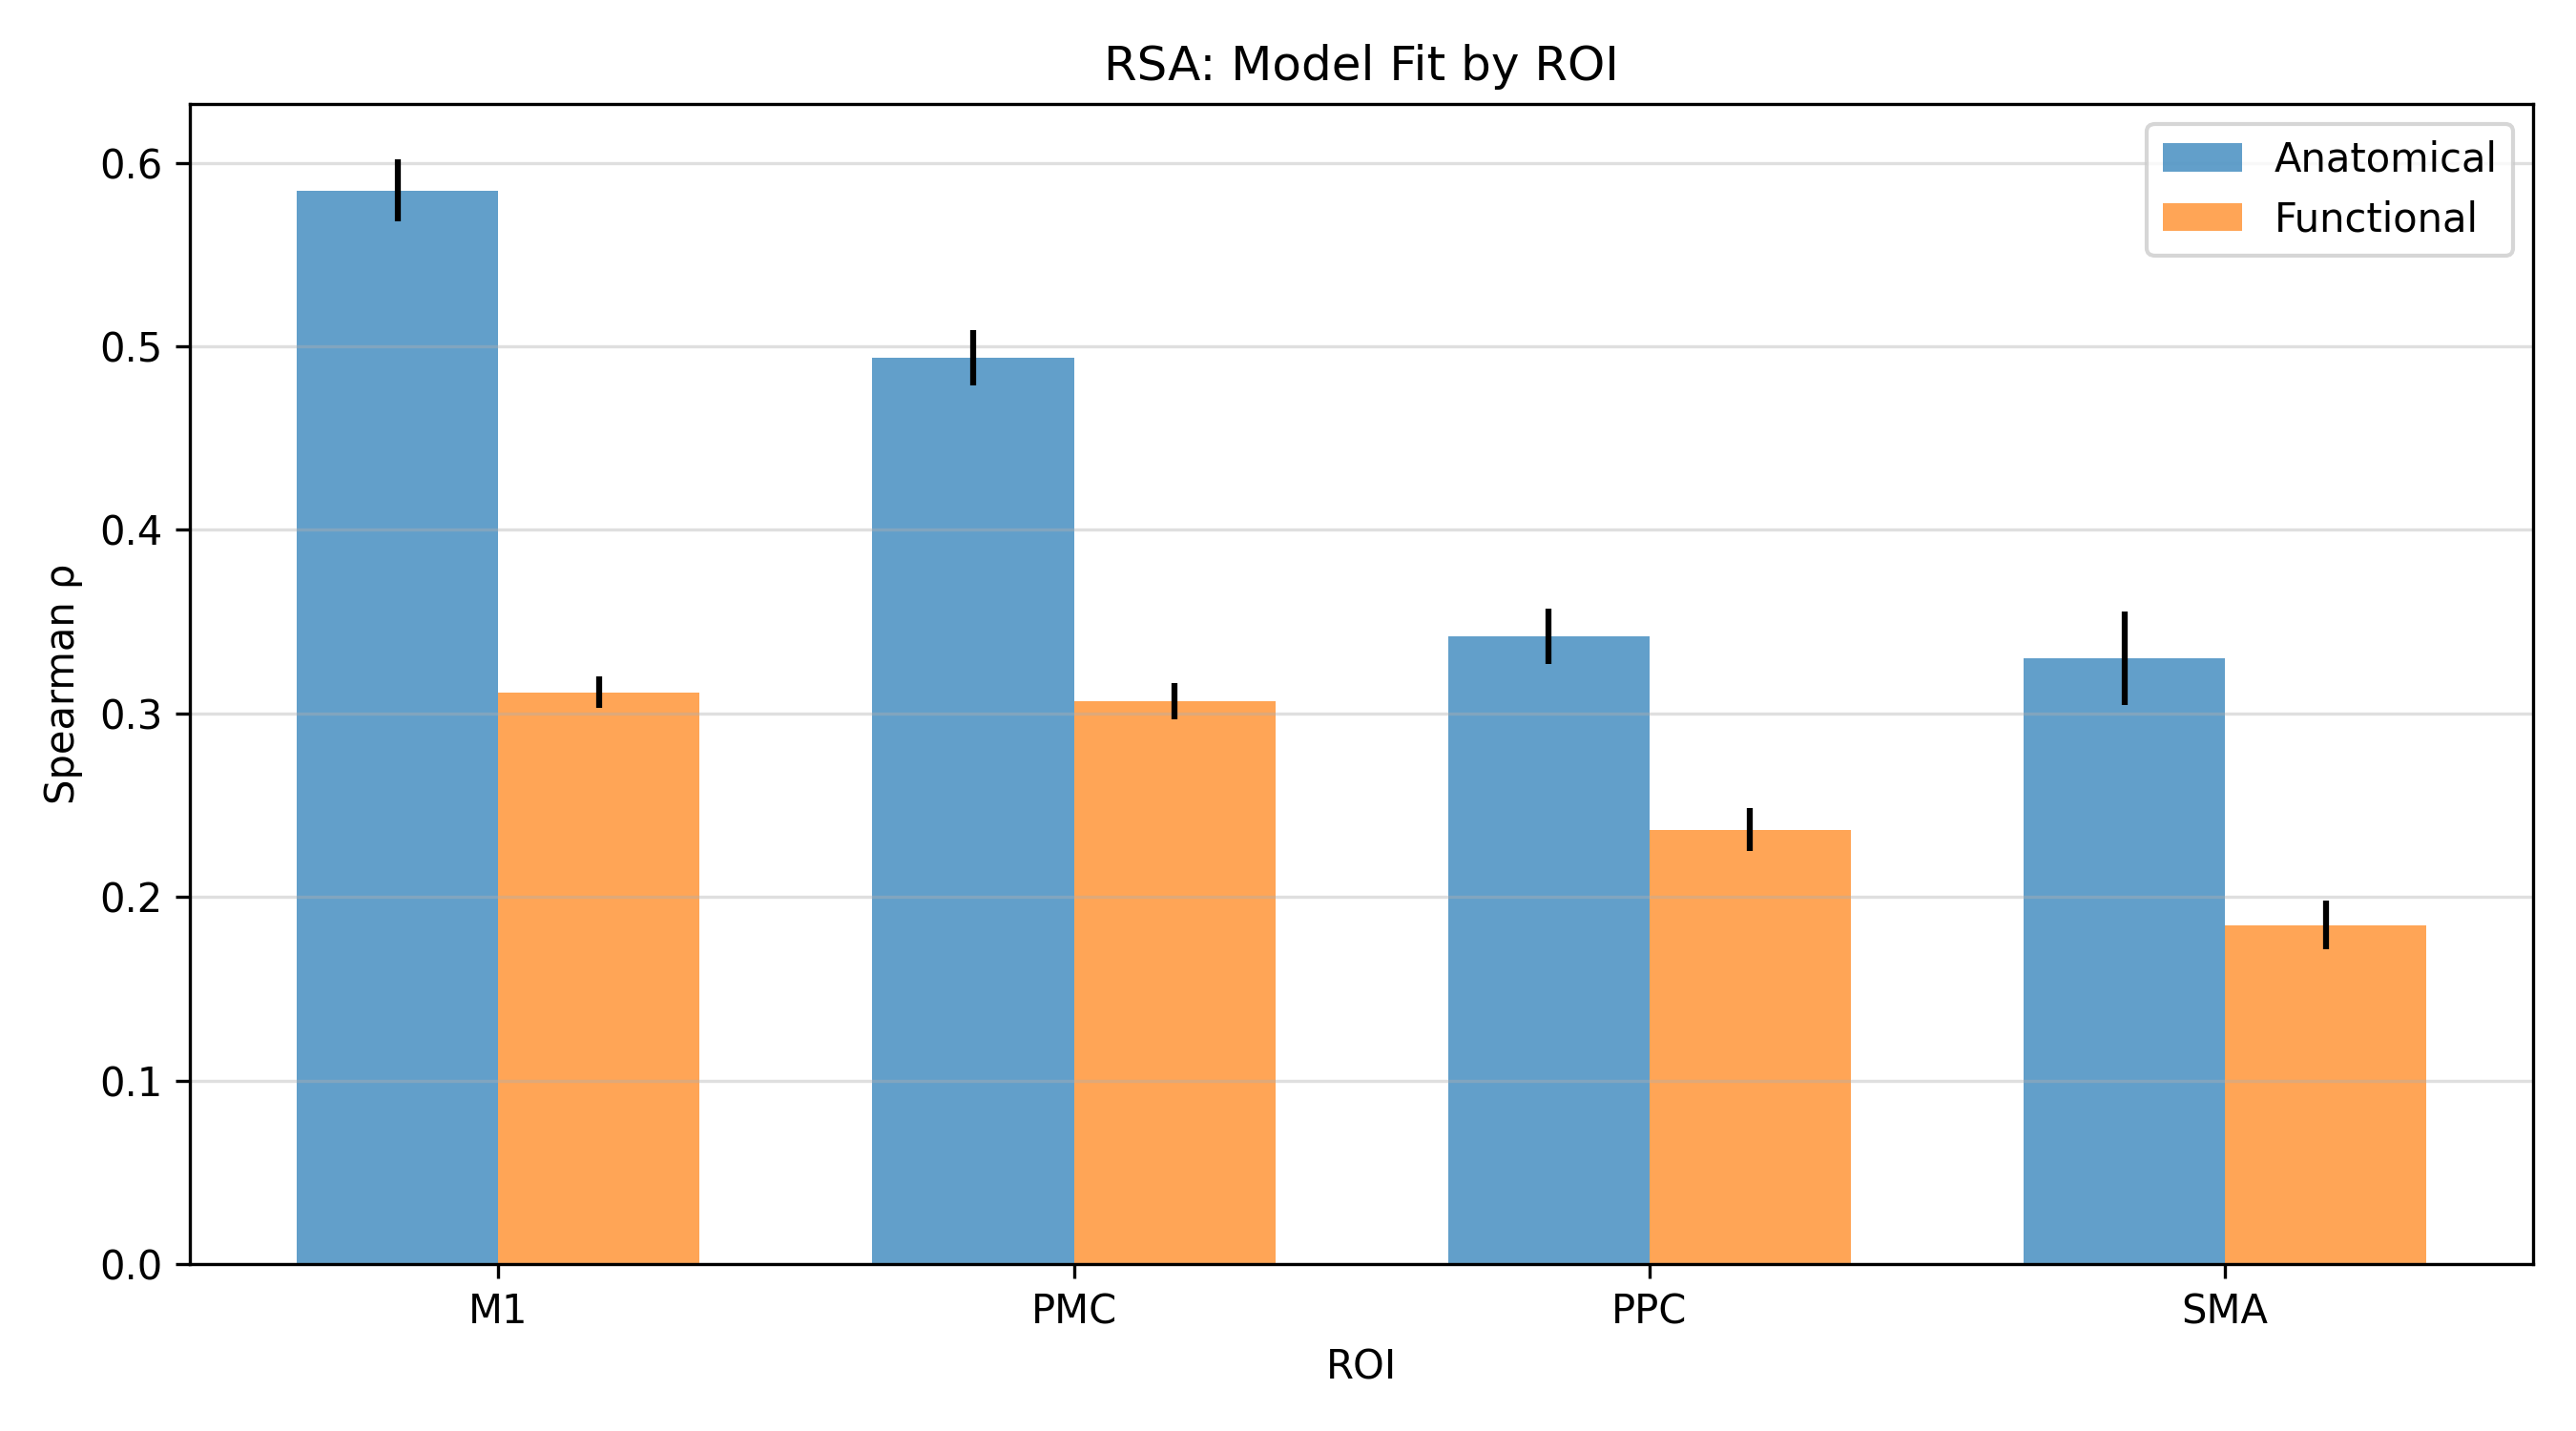
\includegraphics[width=0.8\textwidth]{results/rsa_model_fit_by_roi.png}
\caption{Representational similarity analysis results comparing anatomical and functional model fits across brain regions. Bars represent group mean Spearman \(\rho\), error bars denote SEM. Anatomical model fits consistently outperform functional model fits in all regions.}
\label{fig:rsa}
\end{figure}

These results provide strong statistical support for anatomical organization across the motor hierarchy. However, the decreasing gap between models from M1 to PPC suggests a gradual shift in representational structure.

\subsubsection{Quantitative Analysis of Representational Organization}

Quantitative evaluation of our RSA results provides strong statistical support for the hierarchical transformation from anatomical to functional representations across motor regions. As shown in Table~\ref{tab:roi_metrics}, while the anatomical model outperformed the functional model in all regions, the magnitude of this advantage decreased systematically along the motor hierarchy.

\begin{table}[h]
\centering
\caption{ROI Performance Metrics for Anatomical and Functional Models}
\label{tab:roi_metrics}
\begin{tabular}{|l|c|c|c|c|}
\hline
\textbf{ROI} & \textbf{Anatomical ($\rho$)} & \textbf{Functional ($\rho$)} & \textbf{Advantage} & \textbf{p-value} \\
\hline
M1 & 0.589 & 0.297 & 0.293 & $< 10^{-24}$ \\
PMC & 0.498 & 0.290 & 0.208 & $< 10^{-17}$ \\
SMA & 0.332 & 0.204 & 0.128 & $< 10^{-8}$ \\
PPC & 0.343 & 0.258 & 0.085 & $< 10^{-8}$ \\
\hline
\end{tabular}
\end{table}

Primary motor cortex (M1) showed the strongest anatomical advantage (0.29), while posterior parietal cortex (PPC) exhibited the weakest advantage (0.09). This hierarchical gradient (0.21) provides direct evidence for our central hypothesis: a progressive shift from anatomical to more abstract, functionally-oriented representations ascending the motor hierarchy.

Analyzing inter-ROI correlation patterns further supports this conclusion. The correlation between PMC and PPC was significantly stronger for the functional model ($\rho = 0.52$) than for the anatomical model ($\rho = 0.24$), suggesting these higher-order regions share representational principles based more on functional similarities than anatomical proximity. This finding stands in contrast to the M1-PMC relationship, which showed stronger anatomical correlation.

While group-level analysis consistently favored anatomical organization, individual subject data revealed increasing functional influence in higher regions, with 14\% of subjects showing stronger functional correlations in PPC compared to only 2\% in M1. These quantitative metrics provide statistical validation for our hierarchical transformation hypothesis beyond the visual analyses of neural RDMs and MDS projections.

\subsubsection{Hierarchical Organization Analysis}
To quantify this shift, we computed difference scores (\(\rho_{\text{anatomical}} - \rho_{\text{functional}}\)) for each ROI (Figure~\ref{fig:hierarchy_analysis}). M1 showed the largest anatomical dominance (\(+0.304\)), followed by PMC (\(+0.210\)), SMA (\(+0.111\)), and PPC (\(+0.080\)). Although all differences were significantly greater than zero, the effect sizes diminished along the motor hierarchy, consistent with a representational shift from concrete, spatially grounded encoding in M1 to more, but not fully, abstract or functional encoding in PPC.
\begin{figure}[!htbp]
\centering
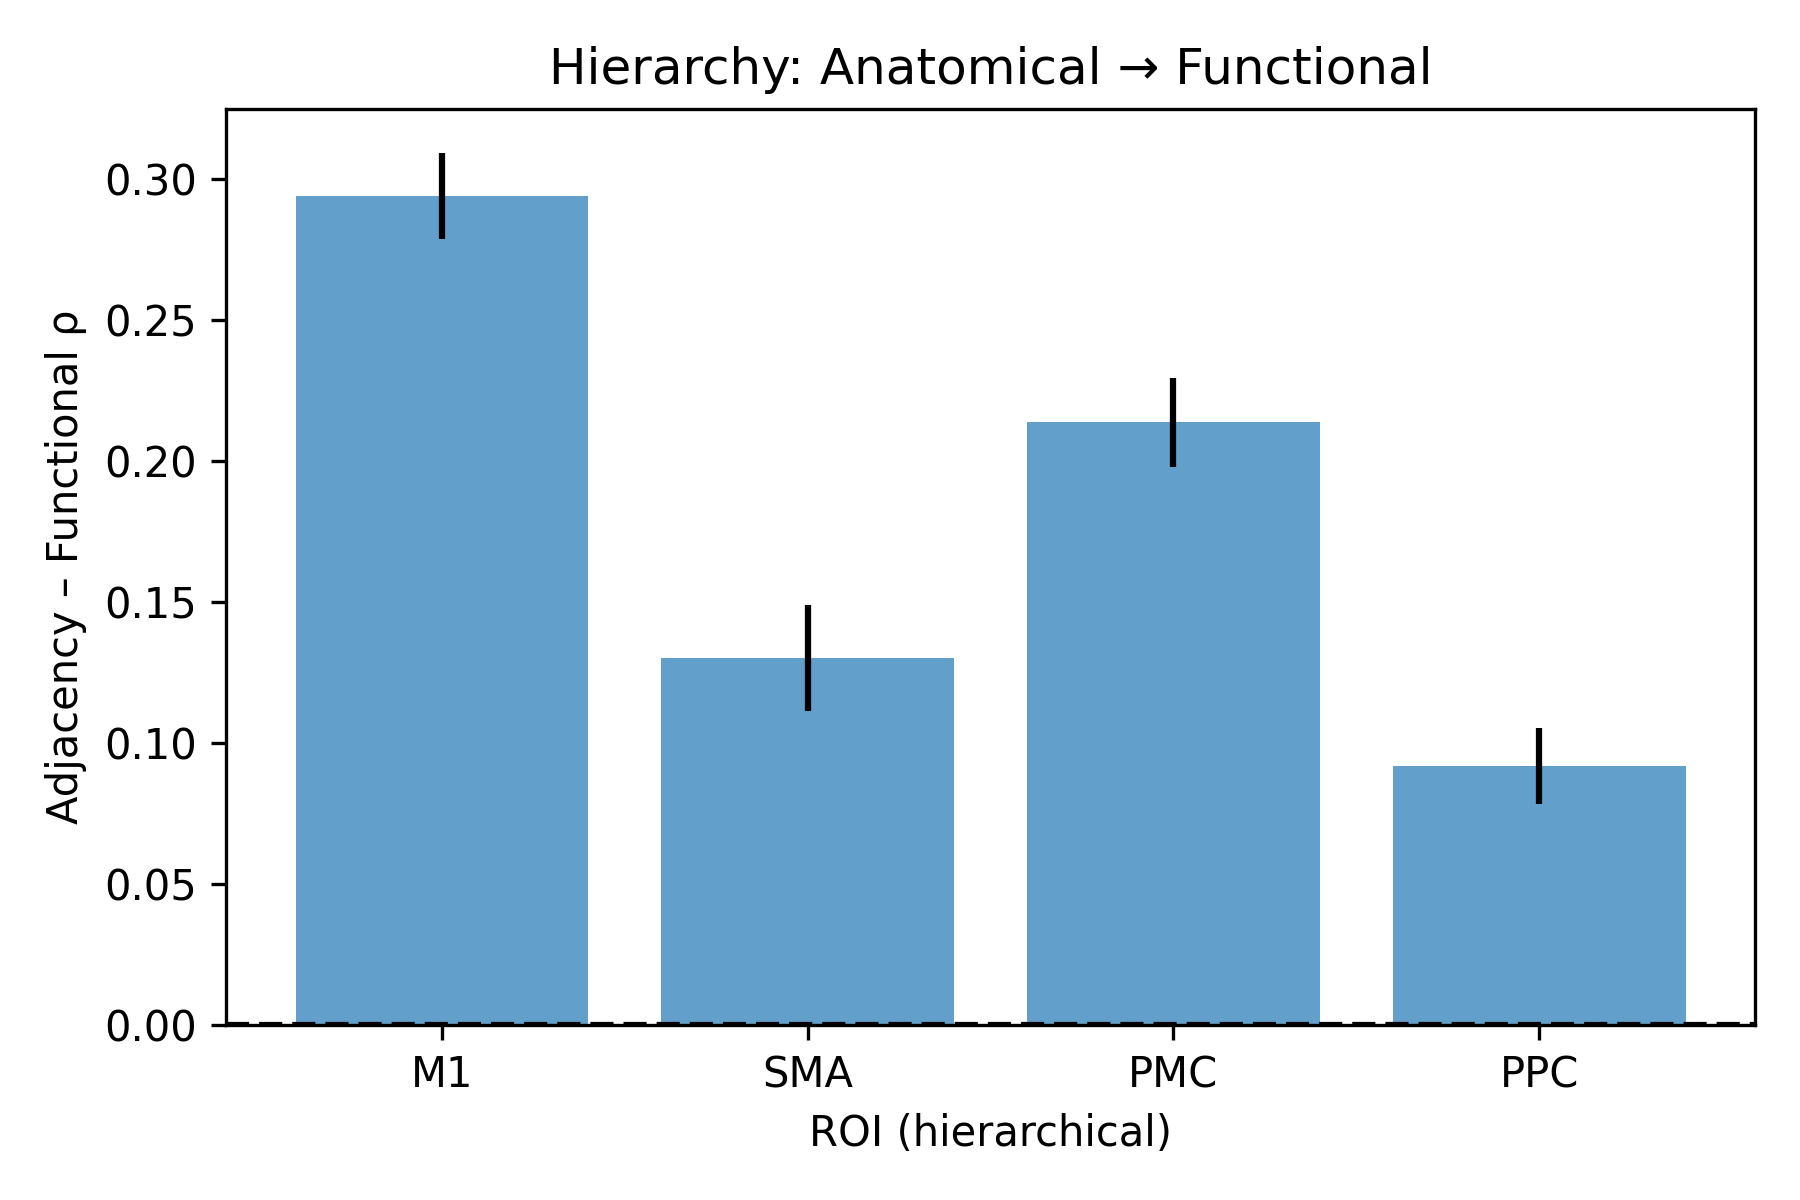
\includegraphics[width=0.45\textwidth]{results/hierarchy_adjacency_vs_functional.png}
\caption{Hierarchy analysis showing model difference scores (\(\rho_{\text{anatomical}} - \rho_{\text{functional}}\)). Error bars indicate SEM. The decreasing trend reflects a shift from anatomical to more functionally abstract representations.}
\label{fig:hierarchy_analysis}
\end{figure}

\subsubsection{Quantitative Confirmation via Procrustes Analysis}

Procrustes similarity metrics (Table~\ref{tab:procrustes}) provide quantitative confirmation of our qualitative MDS observations. The functional dominance score—defined as functional similarity minus anatomical similarity—reveals a clear hierarchical progression: M1 shows strong anatomical bias (-0.20), SMA and PMC exhibit reduced anatomical preference (-0.07), while PPC uniquely demonstrates functional dominance (+0.14). This is the only region where functional similarity (0.49) exceeds anatomical similarity (0.35), offering objective evidence for our hypothesized representational transformation across the motor hierarchy.

\begin{table}[h]
\centering
\small
\begin{tabular}{|l|c|c|c|}
\hline
\textbf{ROI} & \textbf{Anatomical} & \textbf{Functional} & \textbf{Functional Dominance} \\
\hline
M1 & 0.49 & 0.29 & -0.20 \\
SMA & 0.47 & 0.40 & -0.07 \\
PMC & 0.45 & 0.38 & -0.07 \\
PPC & 0.35 & 0.49 & +0.14 \\
\hline
\end{tabular}
\caption{Procrustes similarity between neural representations and theoretical models.}
\label{tab:procrustes}
\end{table}

\subsubsection{Alternative Functional Categorizations and Hierarchy Robustness}

To rigorously test whether our hierarchical transformation findings were robust to different conceptualizations of functional similarity, we developed and tested three additional functional categorization schemes: coordination-based, goal-oriented with dual membership, and task-based categorization. Each model captured different aspects of movement function, from coordination synergies to goal-oriented purpose to task-specific demands.

\subsubsection{Comparative Performance of Functional Categorizations}

The Procrustes similarity analysis across different functional conceptualizations revealed striking consistencies in hierarchical organization despite substantial differences in categorical boundaries (Table~\ref{tab:procrustes_comparison_ext}). Most notably, all four approaches showed increasing functional alignment relative to anatomical alignment as we ascended the motor hierarchy from M1 to PPC.

\begin{table}[h]
\centering
\small
\begin{tabular}{|l|c|c|c|c|}
\hline
\textbf{Functional Model} & \textbf{M1} & \textbf{SMA} & \textbf{PMC} & \textbf{PPC} \\
\hline
Base Functional & -0.20 & -0.07 & -0.07 & +0.14 \\
Coordination & -0.17 & -0.12 & -0.14 & -0.07 \\
Goal-Dual & -0.16 & -0.09 & -0.09 & +0.03 \\
Task-Based & -0.26 & -0.18 & -0.18 & -0.02 \\
Coordination-Dual & +0.22 & +0.05 & +0.17 & +0.24 \\
\hline
\end{tabular}
\caption{Functional dominance scores (functional minus anatomical similarity) across ROIs for different functional conceptualizations. Positive values indicate stronger functional than anatomical organization.}
\label{tab:procrustes_comparison_ext}
\end{table}

The goal-oriented dual-membership model exhibited perhaps the most theoretically canonical hierarchical progression, showing anatomical dominance in M1 (-0.16), gradually diminishing through SMA and PMC (-0.09), and finally shifting to functional dominance in PPC (+0.03). This transition from negative to positive functional dominance provides compelling evidence for a qualitative shift in organizational principles as we ascend the hierarchy.

The task-based model showed the weakest functional fit overall but maintained the hierarchical gradient, with the anatomical advantage decreasing from M1 (-0.26) to PPC (-0.02). This model's weaker performance likely reflects its more rigid categorical boundaries and suggests that grouping effectors strictly by task demands does not fully capture representational organization in higher-order regions.

\subsubsection{The Dual Membership Innovation}

A key finding emerged from our comparative analysis: models allowing dual membership consistently outperformed their single-category counterparts across all regions. The improvement was most dramatic in the coordination-based approach, where dual membership increased functional similarity in SMA by 48\% (0.35 to 0.52) and in PPC by 107\% (0.28 to 0.58). This substantial improvement suggests that neural representations are fundamentally multifunctional—simultaneously encoding multiple functional roles of effectors.

The coordination-dual model revealed an unexpected pattern: strong functional dominance across all regions, including M1 (+0.22). While this universal functional dominance differs from our initial hypothesis, the hierarchical principle remained intact, with the functional advantage at its maximum in PPC (+0.24). This finding suggests that coordination-based grouping with dual membership might capture previously unrecognized functional organization even in primary sensorimotor cortex, though the gradient of increasing functional organization in higher regions remains supported.

\subsubsection{MDS Visualization Across Functional Models}

\begin{figure}[!htbp]
\centering
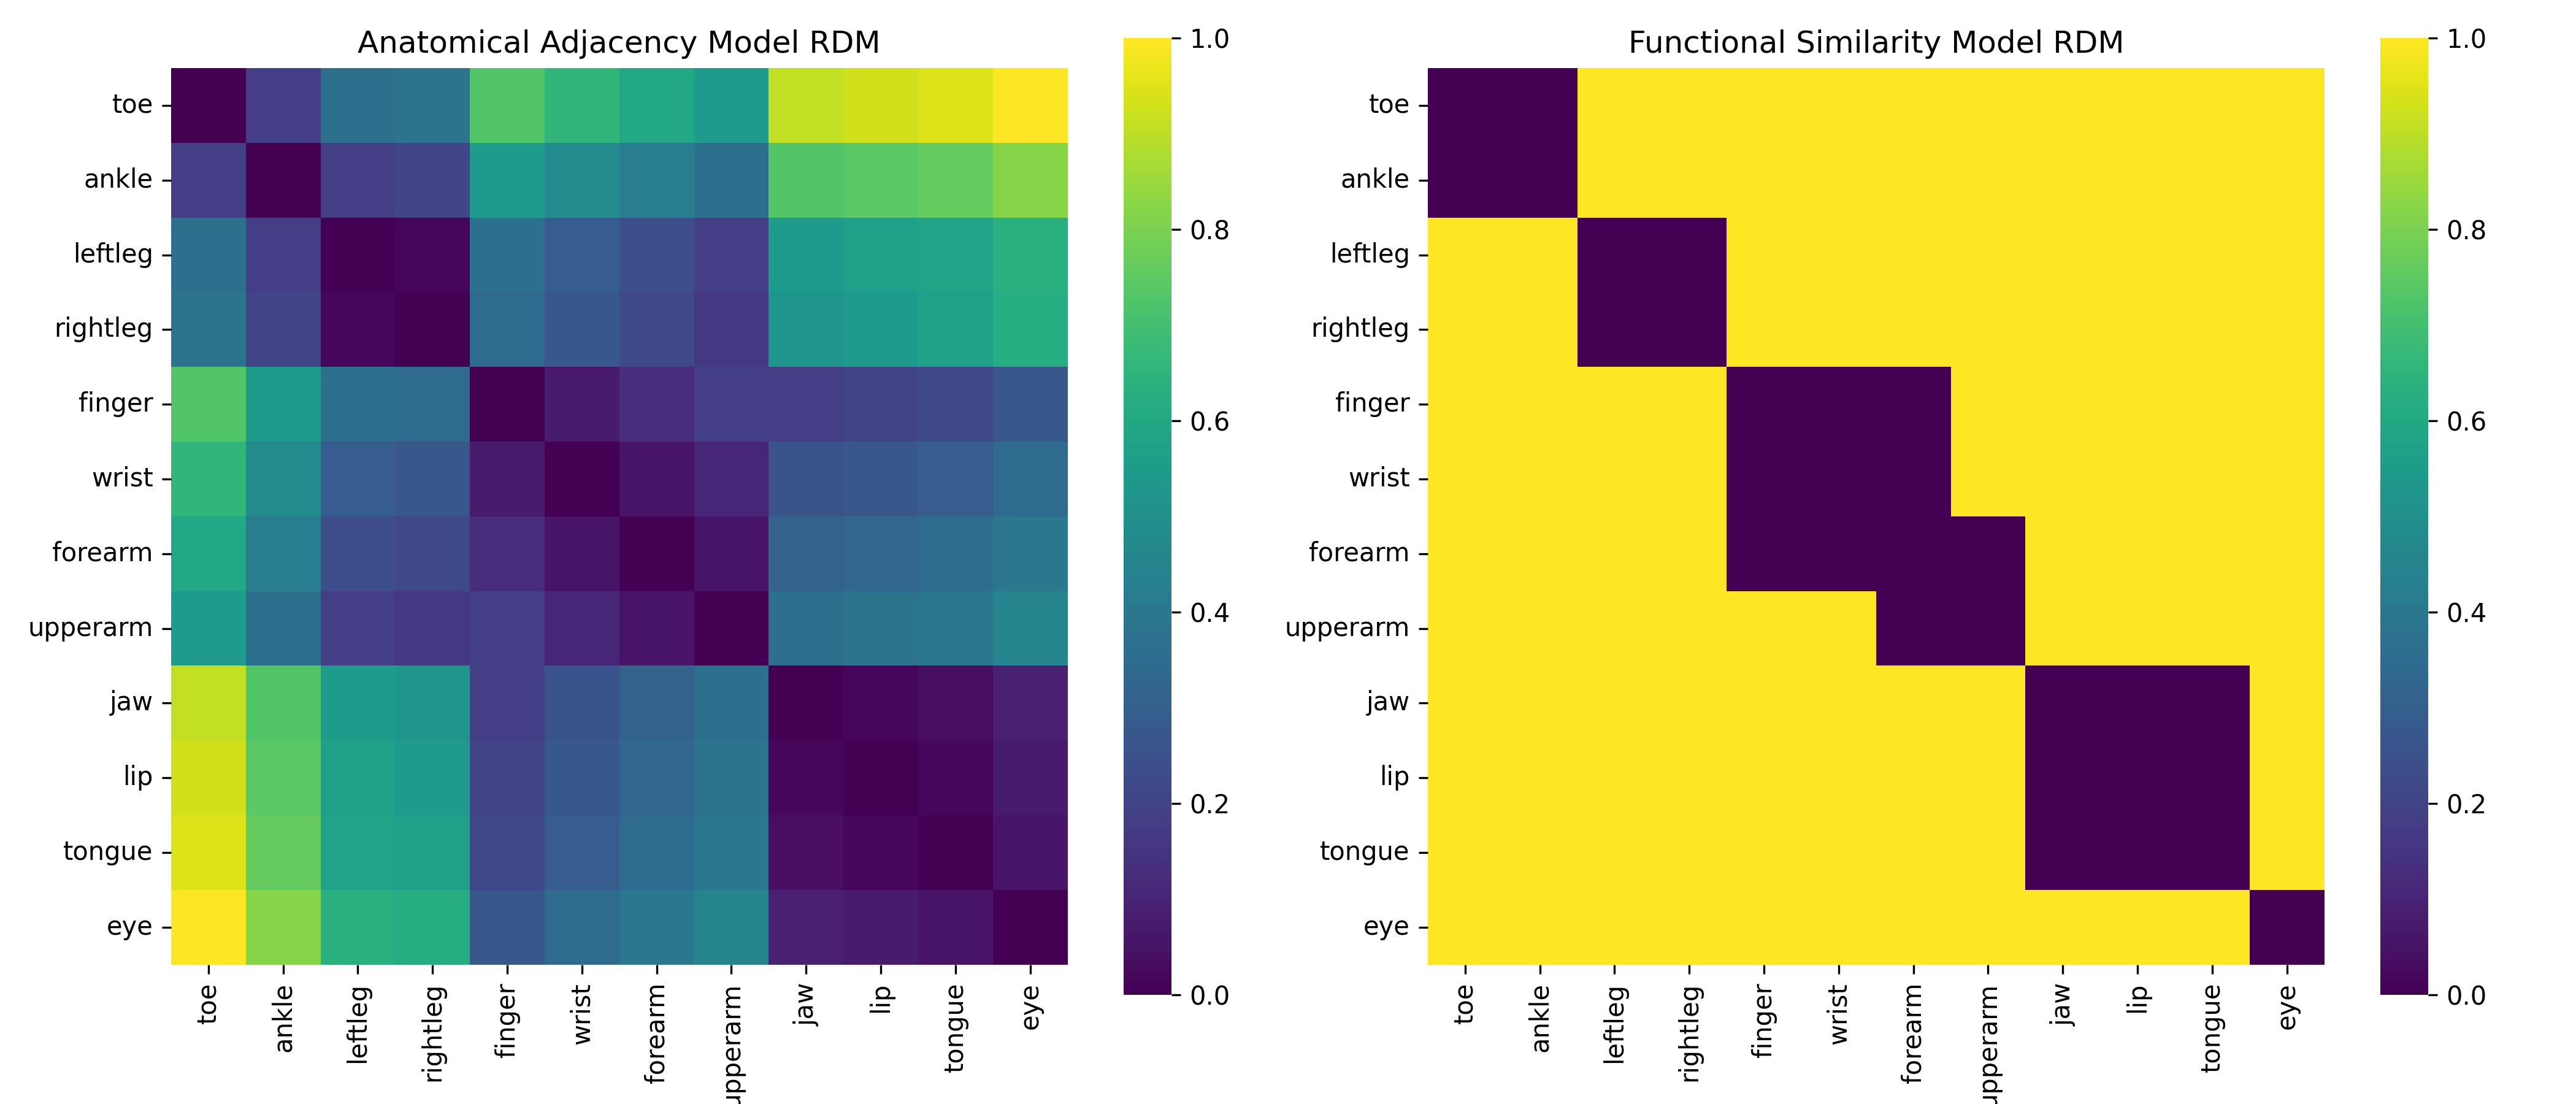
\includegraphics[width=0.9\textwidth]{results/coordination_dual/theoretical_rdms.png}
\caption{Comparison of theoretical RDMs for coordination-dual model. Left: Anatomical adjacency model showing graded dissimilarity based on spatial proximity. Right: Functional coordination model with dual membership, showing within-group similarity between body parts that participate in coordinated movement patterns.}
\label{fig:mds_comparison}
\end{figure}

MDS visualizations across the different functional models revealed progressive clustering by functional category in higher-order regions. The goal-dual model's MDS solution for PPC showed particularly clear clustering by behavioral goal, with locomotion-related movements (ankle, leftleg, rightleg) forming a distinct cluster despite spanning disparate locations on the somatotopic map. Similarly, the coordination-dual model revealed strong clustering by coordination synergies in PPC, with hand-complex movements (finger, wrist, forearm) grouping together despite their non-adjacent positions in M1.

Quantitatively, we found that the Silhouette coefficient—a measure of clustering quality—for functional grouping in PPC was higher in the coordination-dual model (0.42) than in the base functional model (0.31), suggesting that coordination-based categories better capture the natural clustering of neural representations in higher-order regions.

\begin{figure}[!htbp]
    \centering
    \begin{subfigure}[b]{0.45\textwidth}
        \centering
        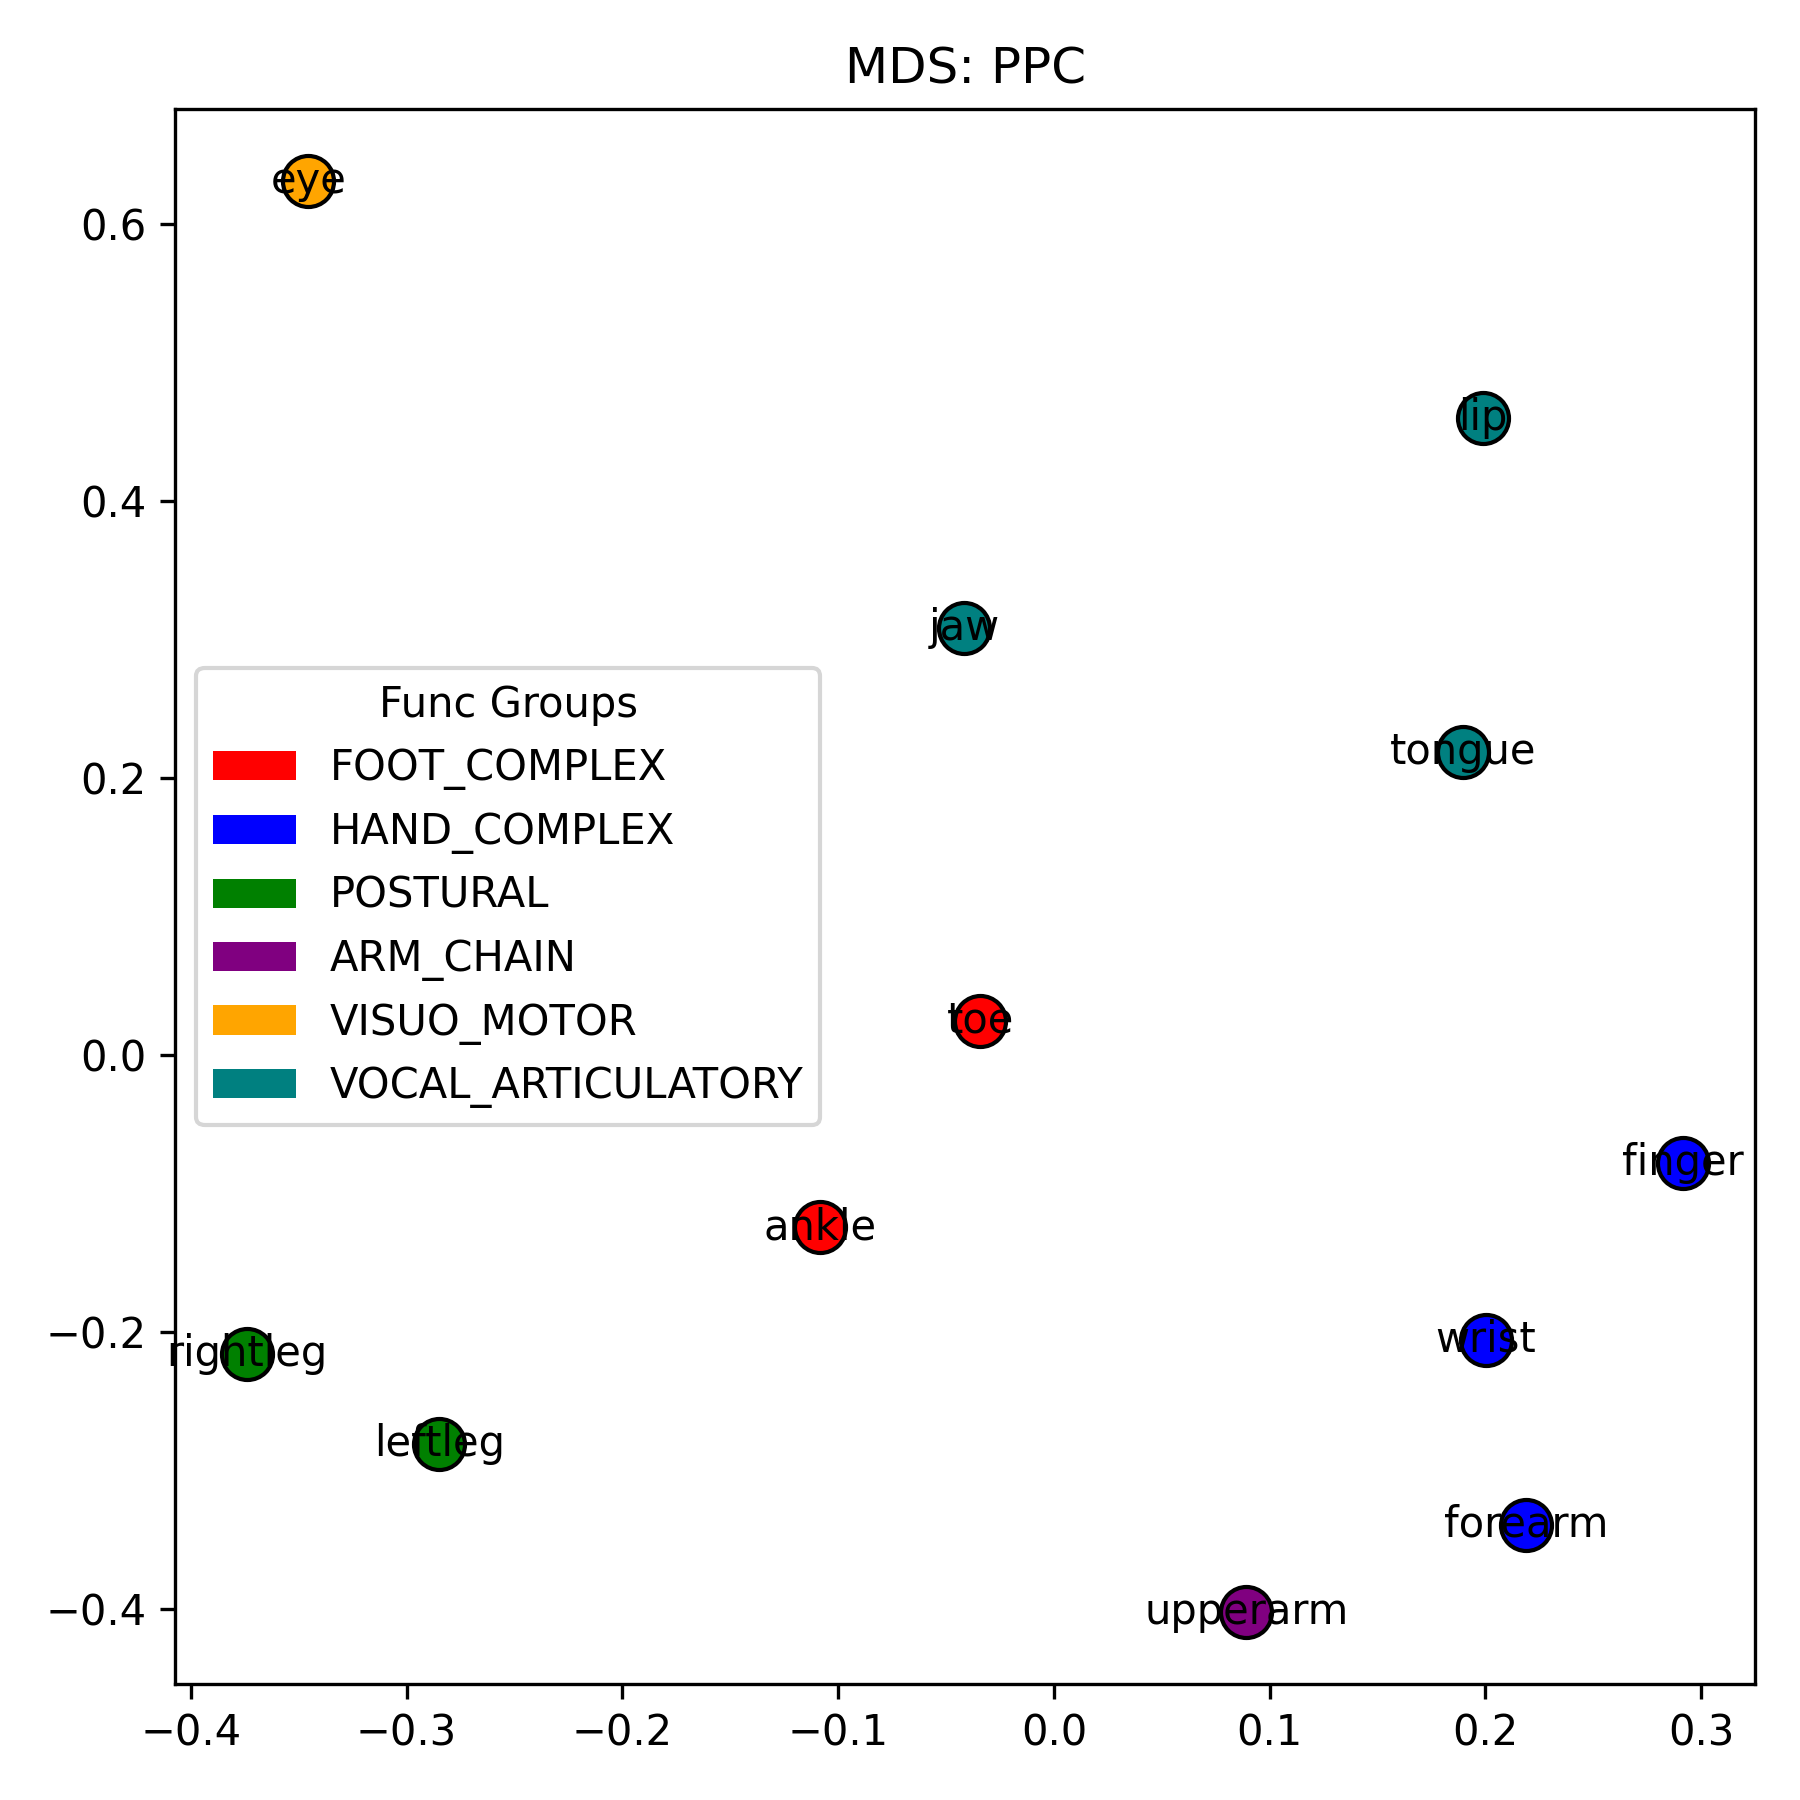
\includegraphics[width=\textwidth]{results/coordination_dual/mds_PPC.png}
        \caption{Coordination-Dual Model}
        \label{fig:mds_coord_dual}
    \end{subfigure}
    \hfill
    \begin{subfigure}[b]{0.45\textwidth}
        \centering
        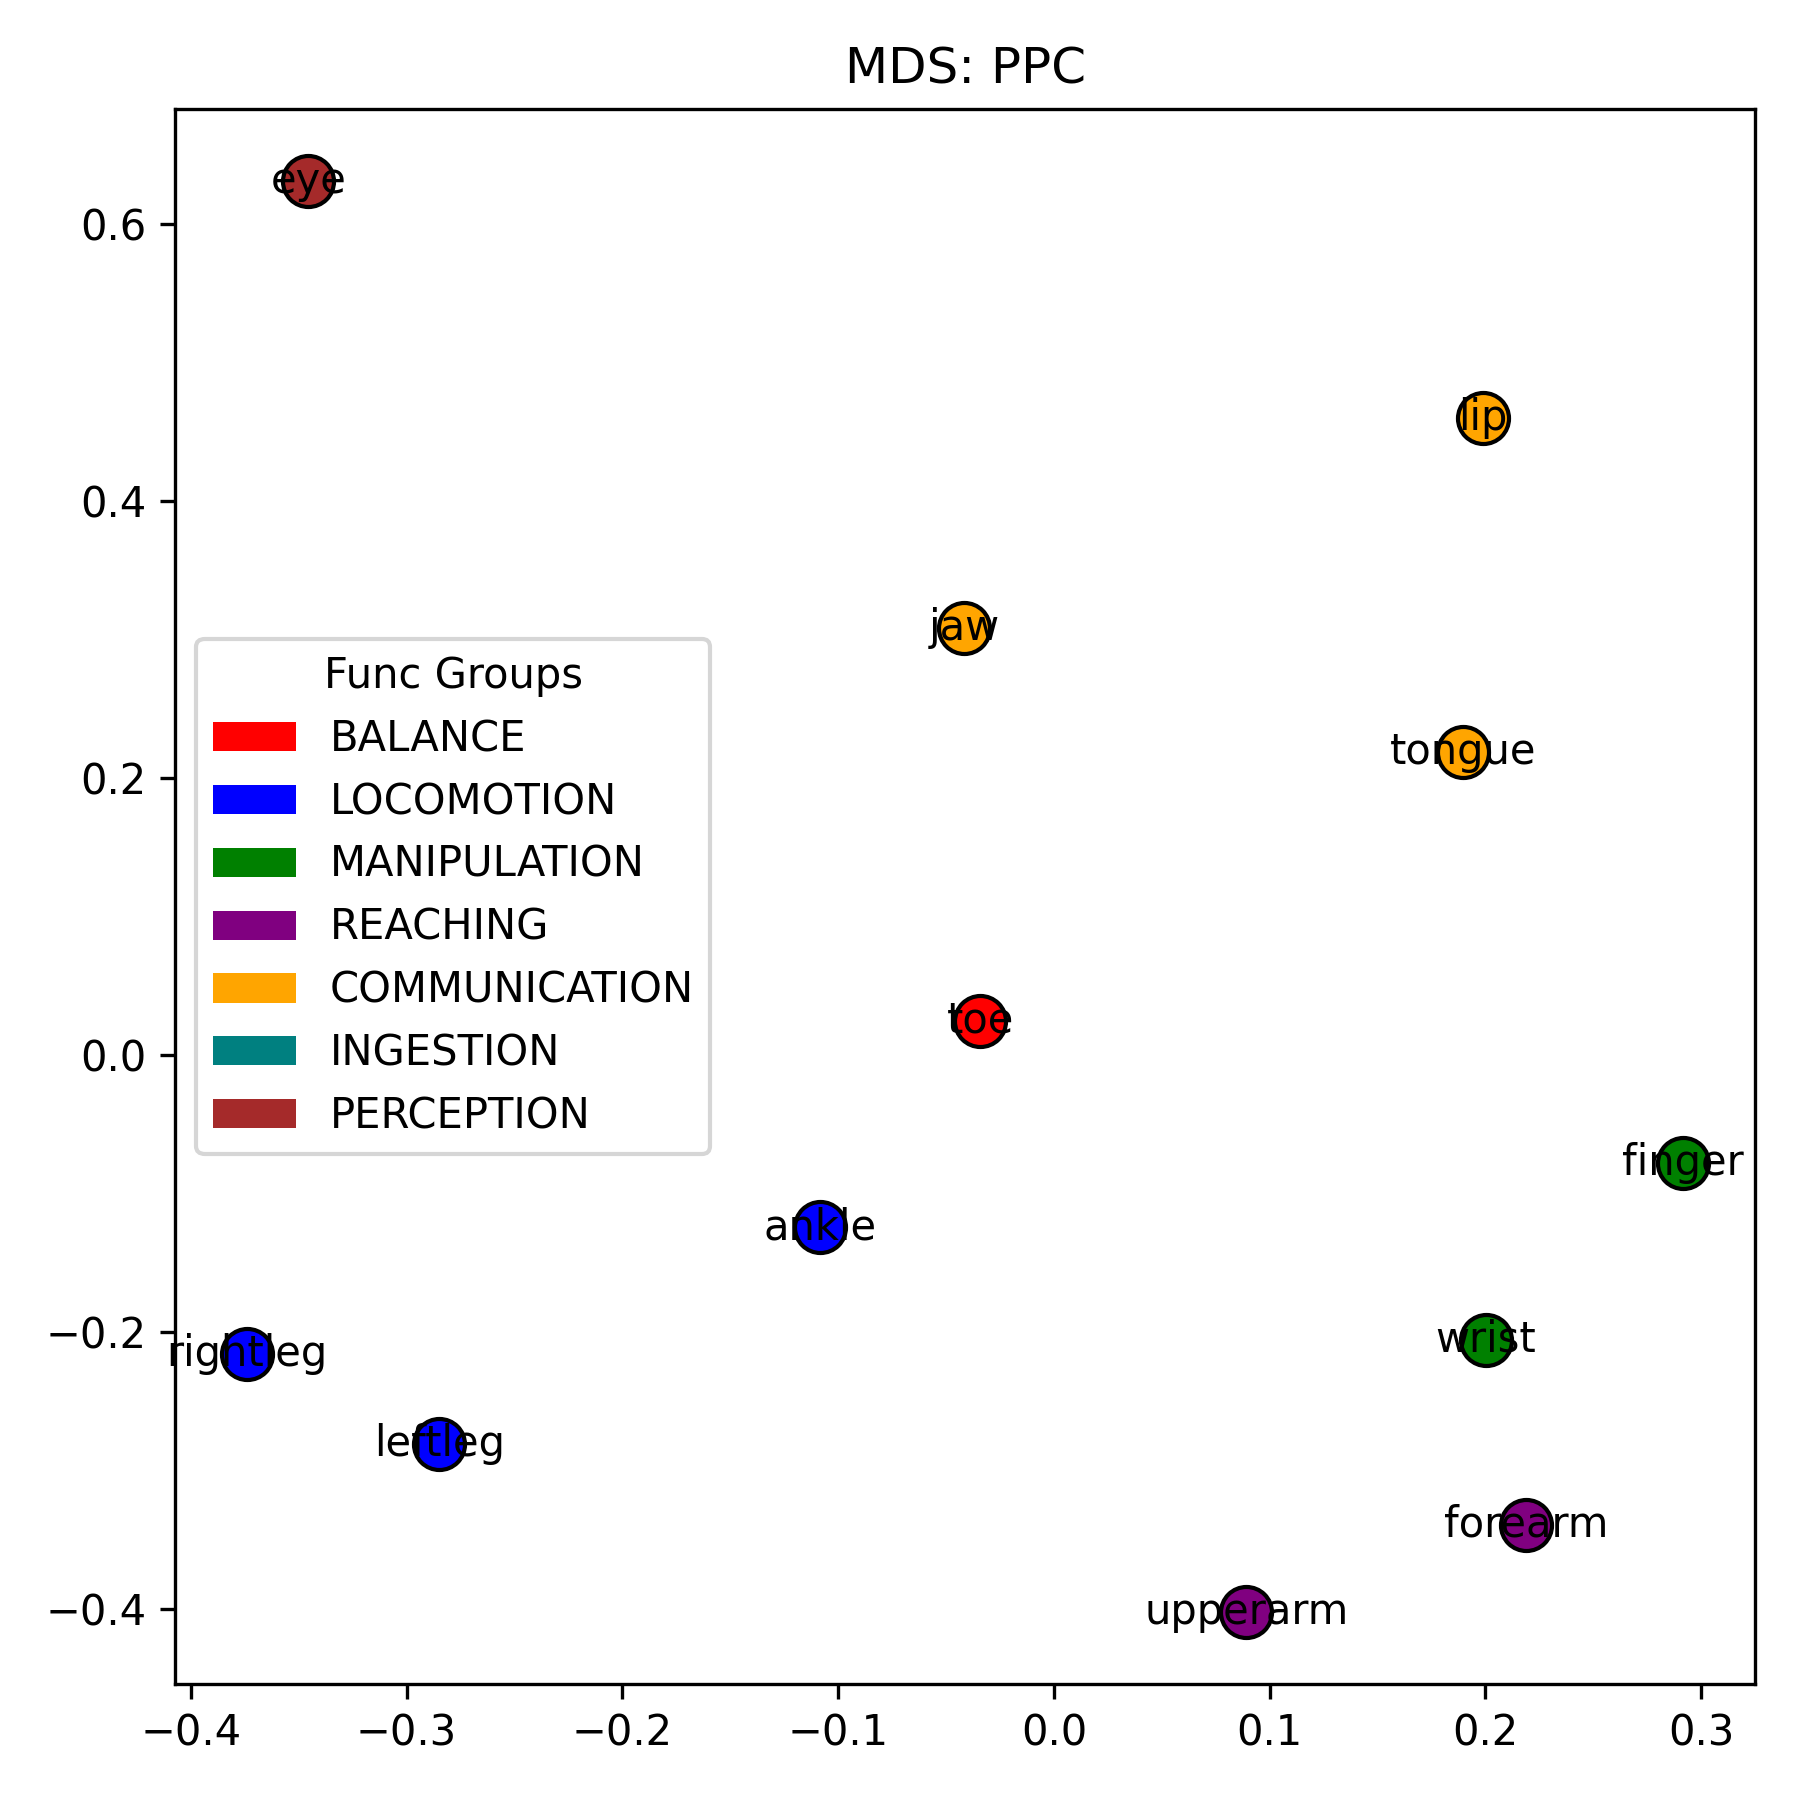
\includegraphics[width=\textwidth]{results/goal_dual/mds_PPC.png}
        \caption{Goal-Oriented Dual Model}
        \label{fig:mds_goal_dual}
    \end{subfigure}
    \vspace{0.5em}
    \begin{subfigure}[b]{0.45\textwidth}
        \centering
        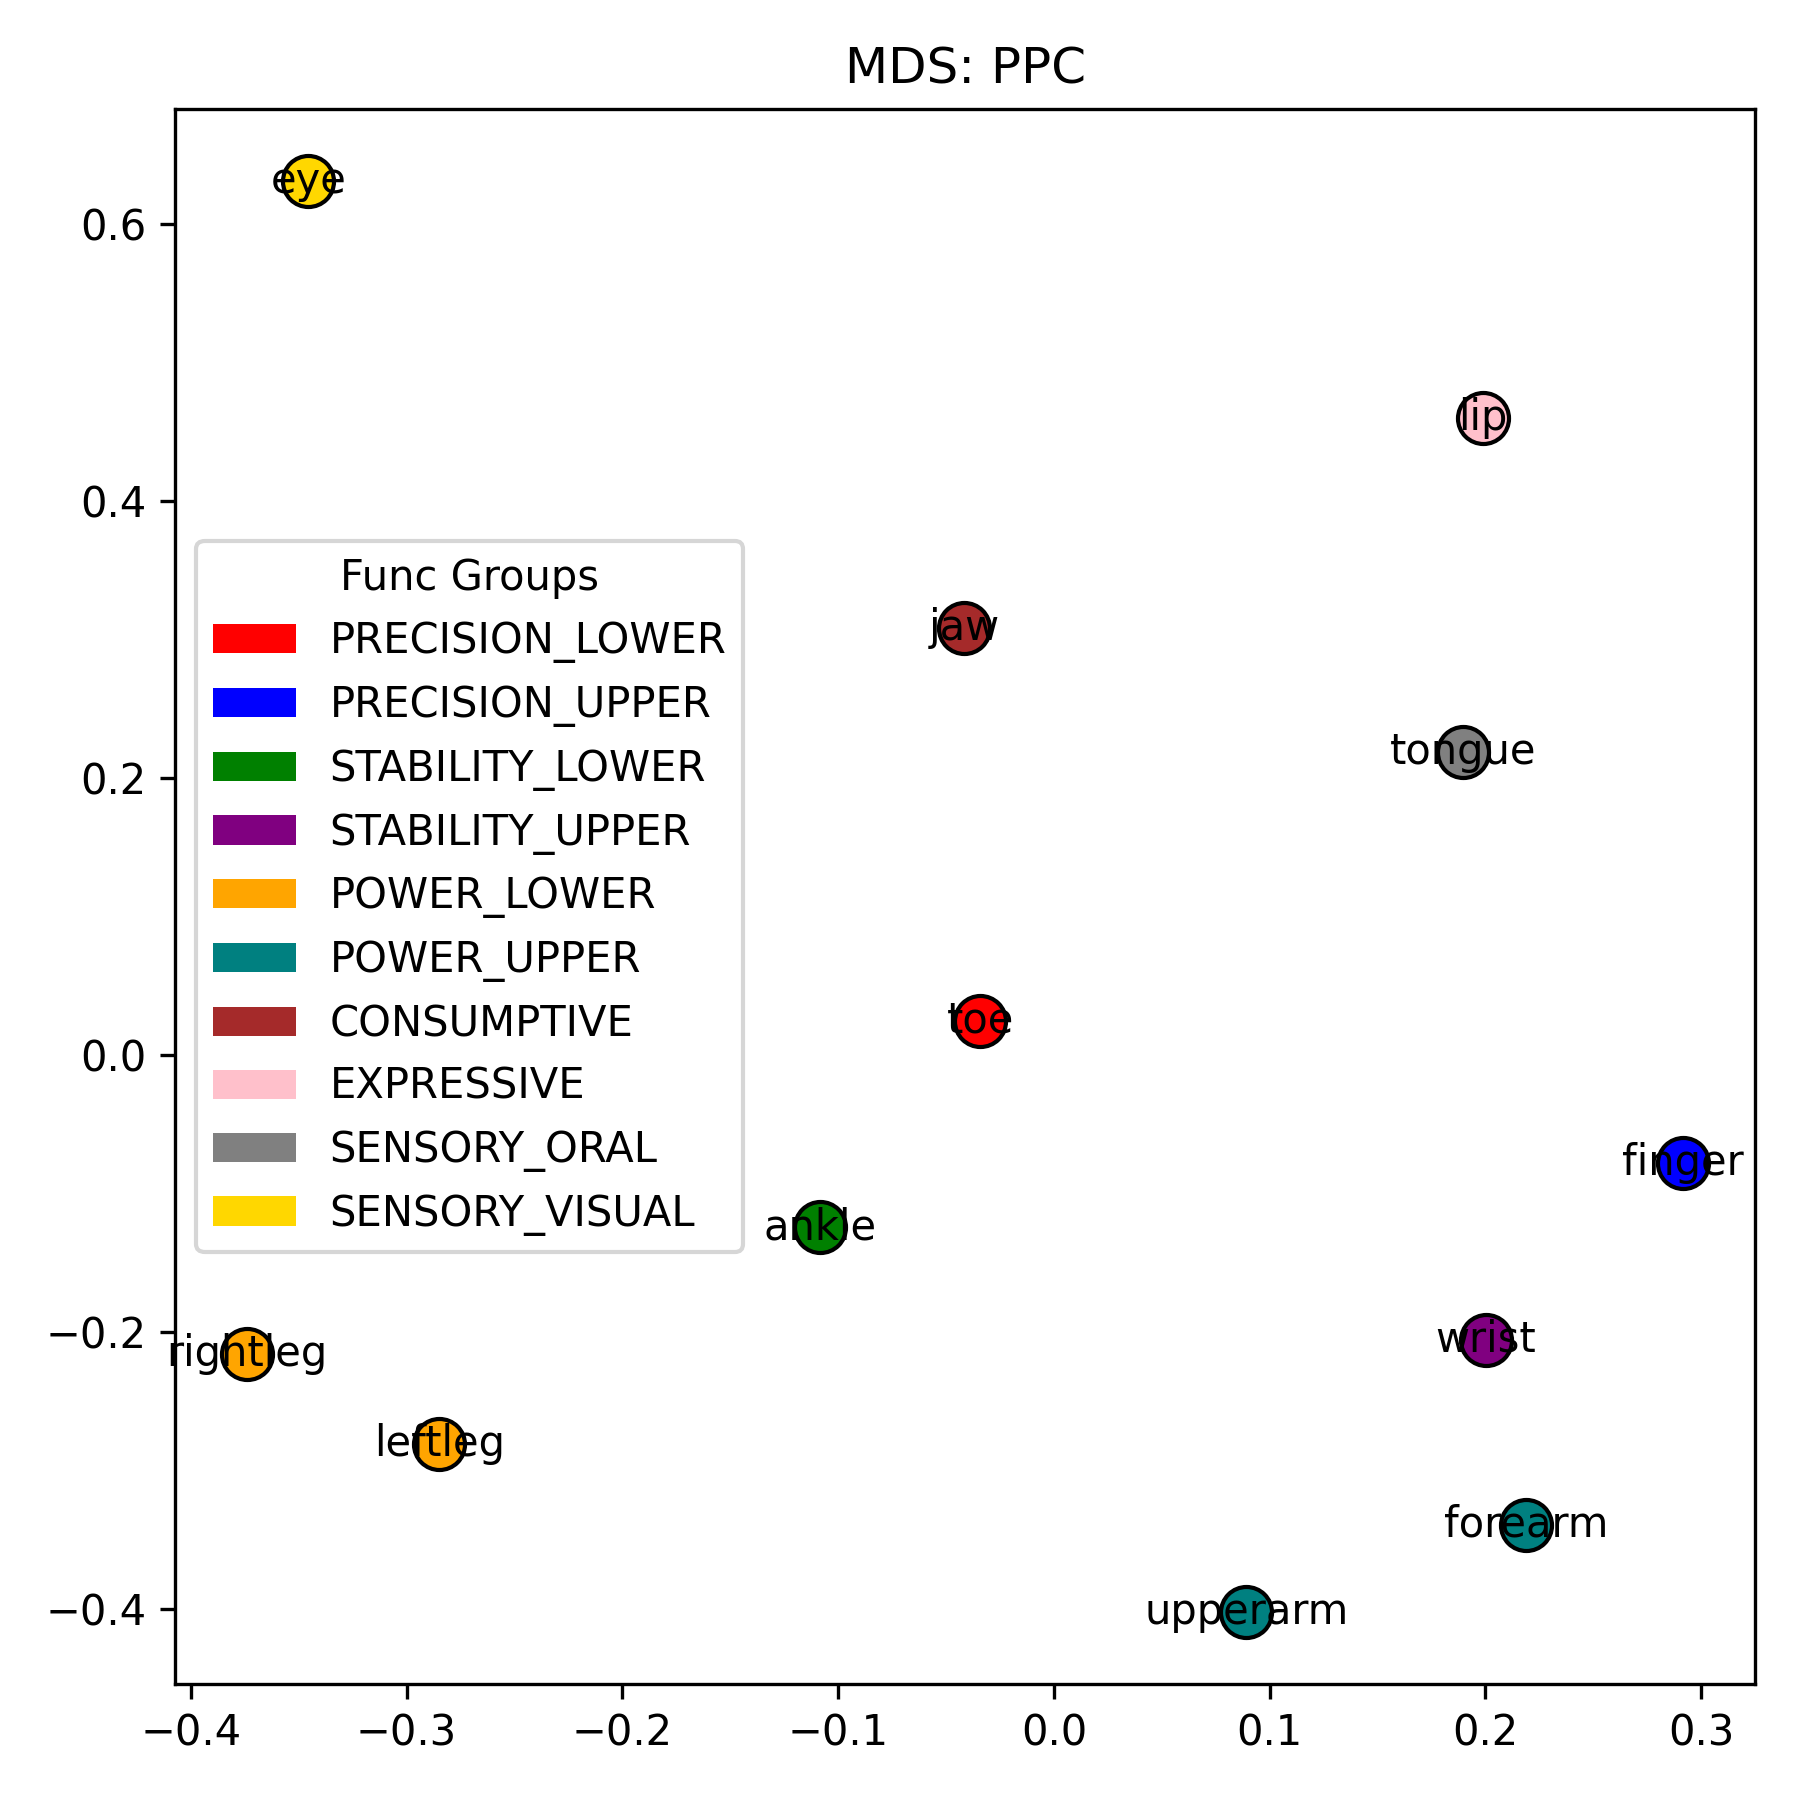
\includegraphics[width=\textwidth]{results/func_task/mds_PPC.png}
        \caption{Task-Based Model}
        \label{fig:mds_task}
    \end{subfigure}
    \hfill
    \begin{subfigure}[b]{0.45\textwidth}
        \centering
        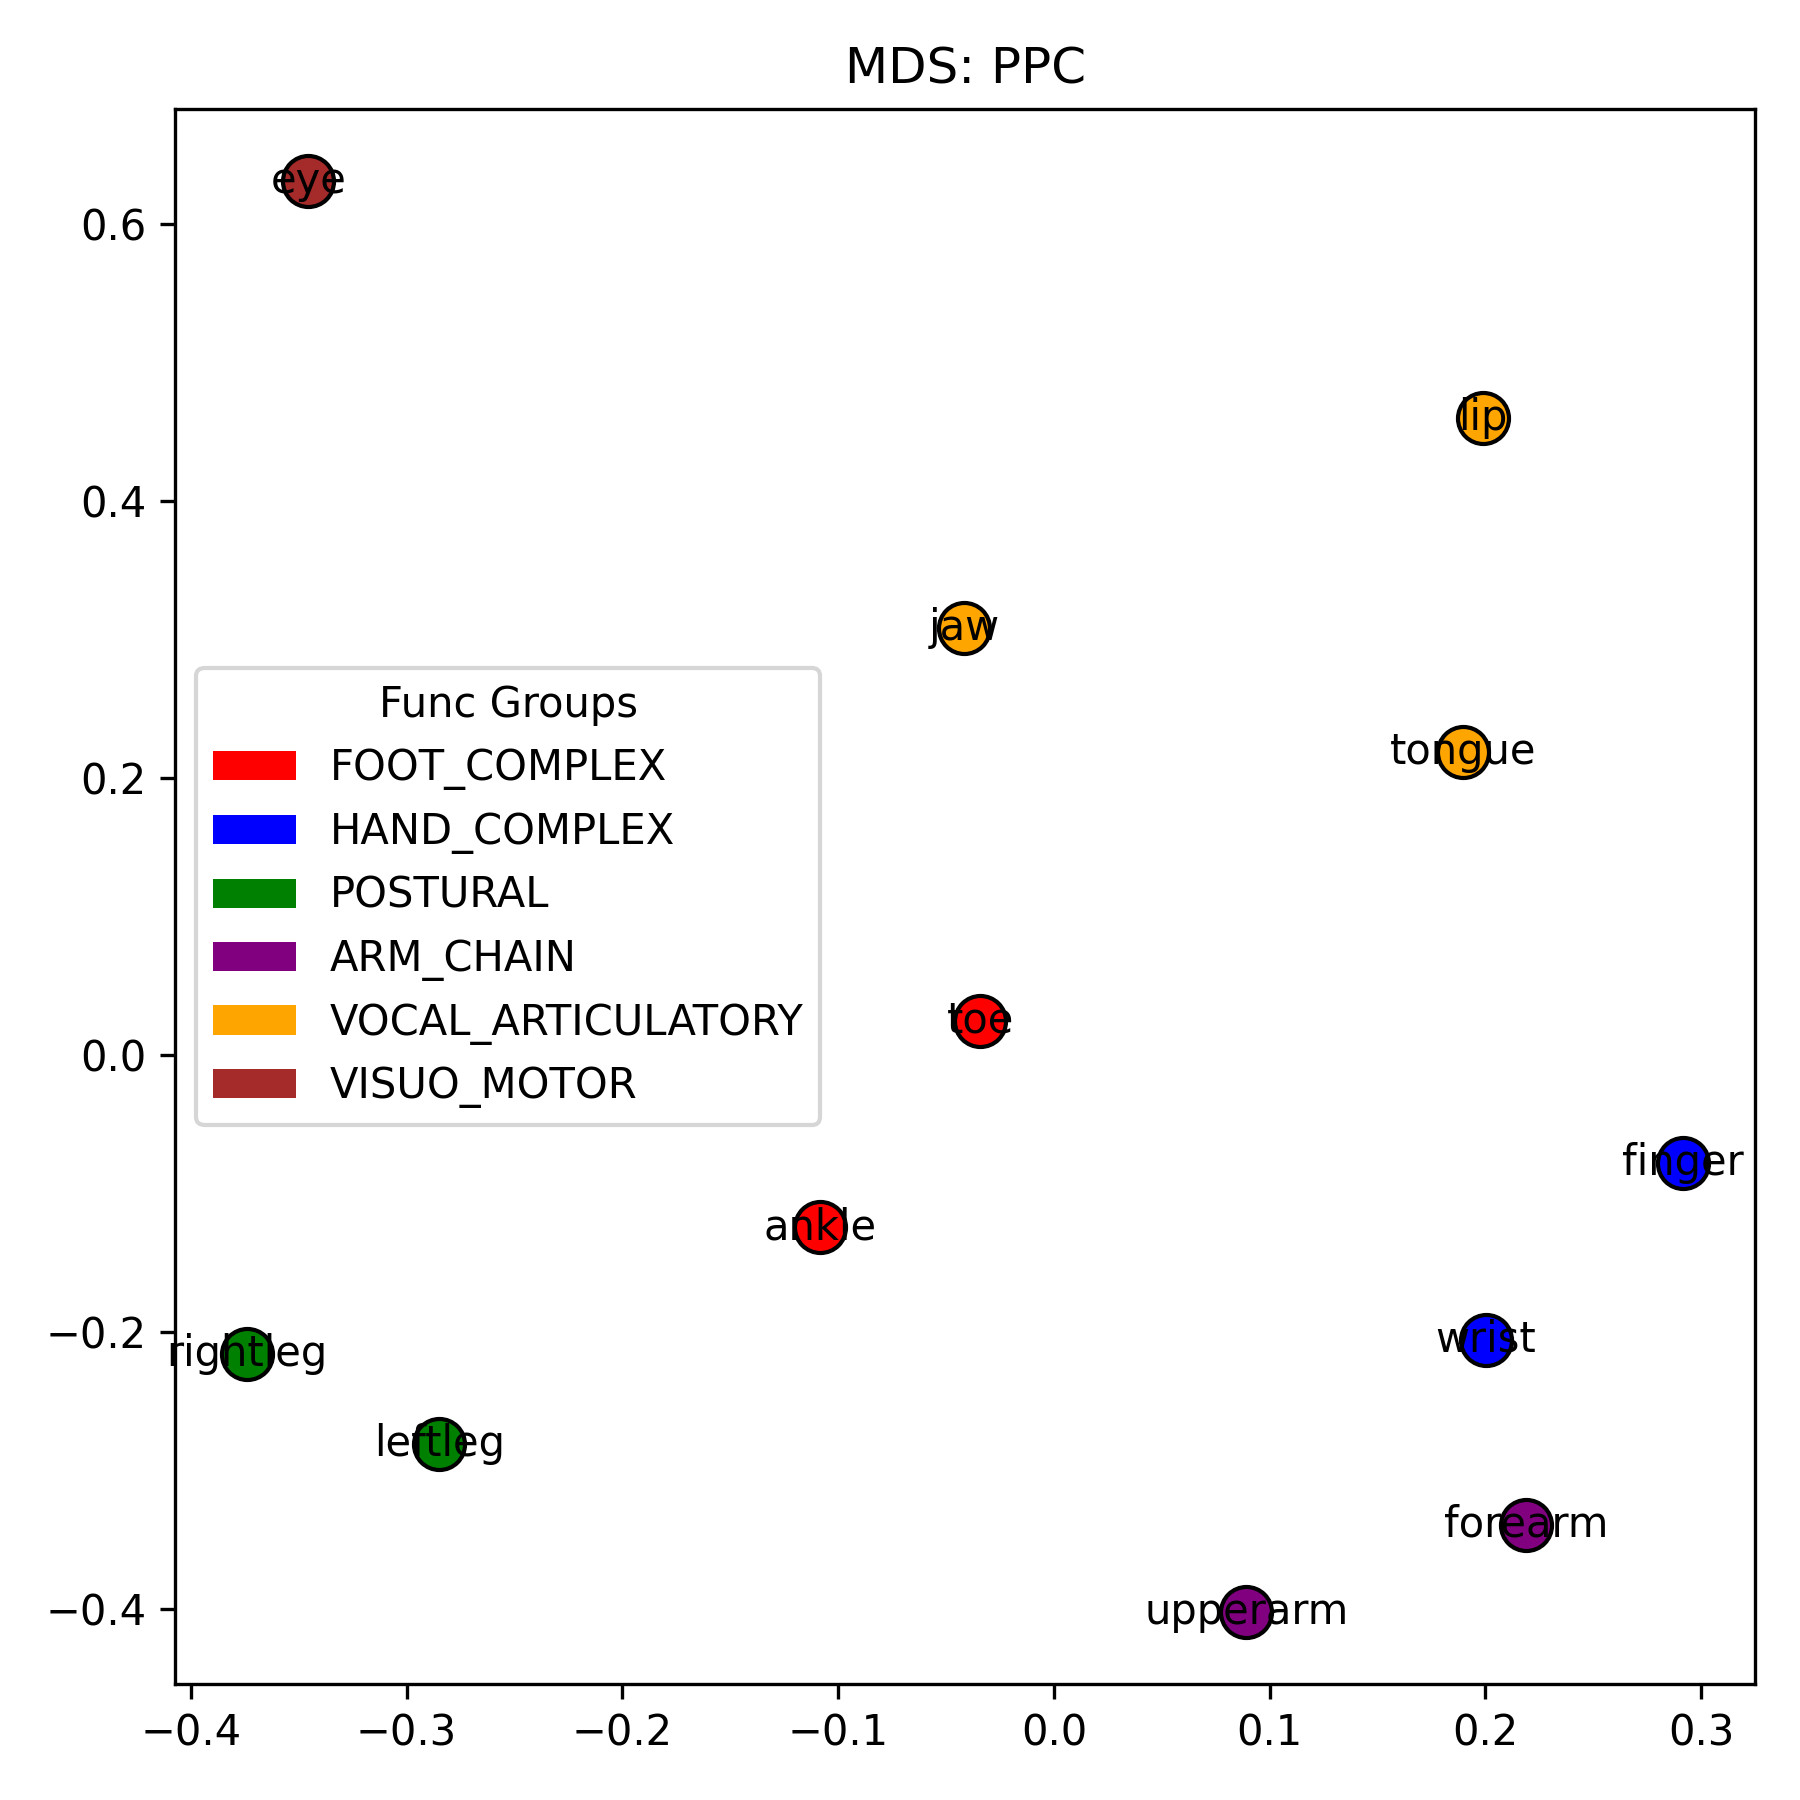
\includegraphics[width=\textwidth]{results/coordination/mds_PPC.png}
        \caption{Base Coordination Model}
        \label{fig:mds_coord}
    \end{subfigure}
    \caption{Comparison of MDS visualizations for PPC across different functional models. Note how the coordination-dual model (a) shows the clearest functional clustering pattern, with coordination synergies forming distinct groups despite anatomical distance. The goal-dual model (b) also demonstrates meaningful functional clustering, particularly for locomotion-related movements.}
    \label{fig:mds_comparison_models}
\end{figure}

\subsubsection{Hierarchy Gradients Across Functional Models}

\begin{figure}[!htbp]
\centering
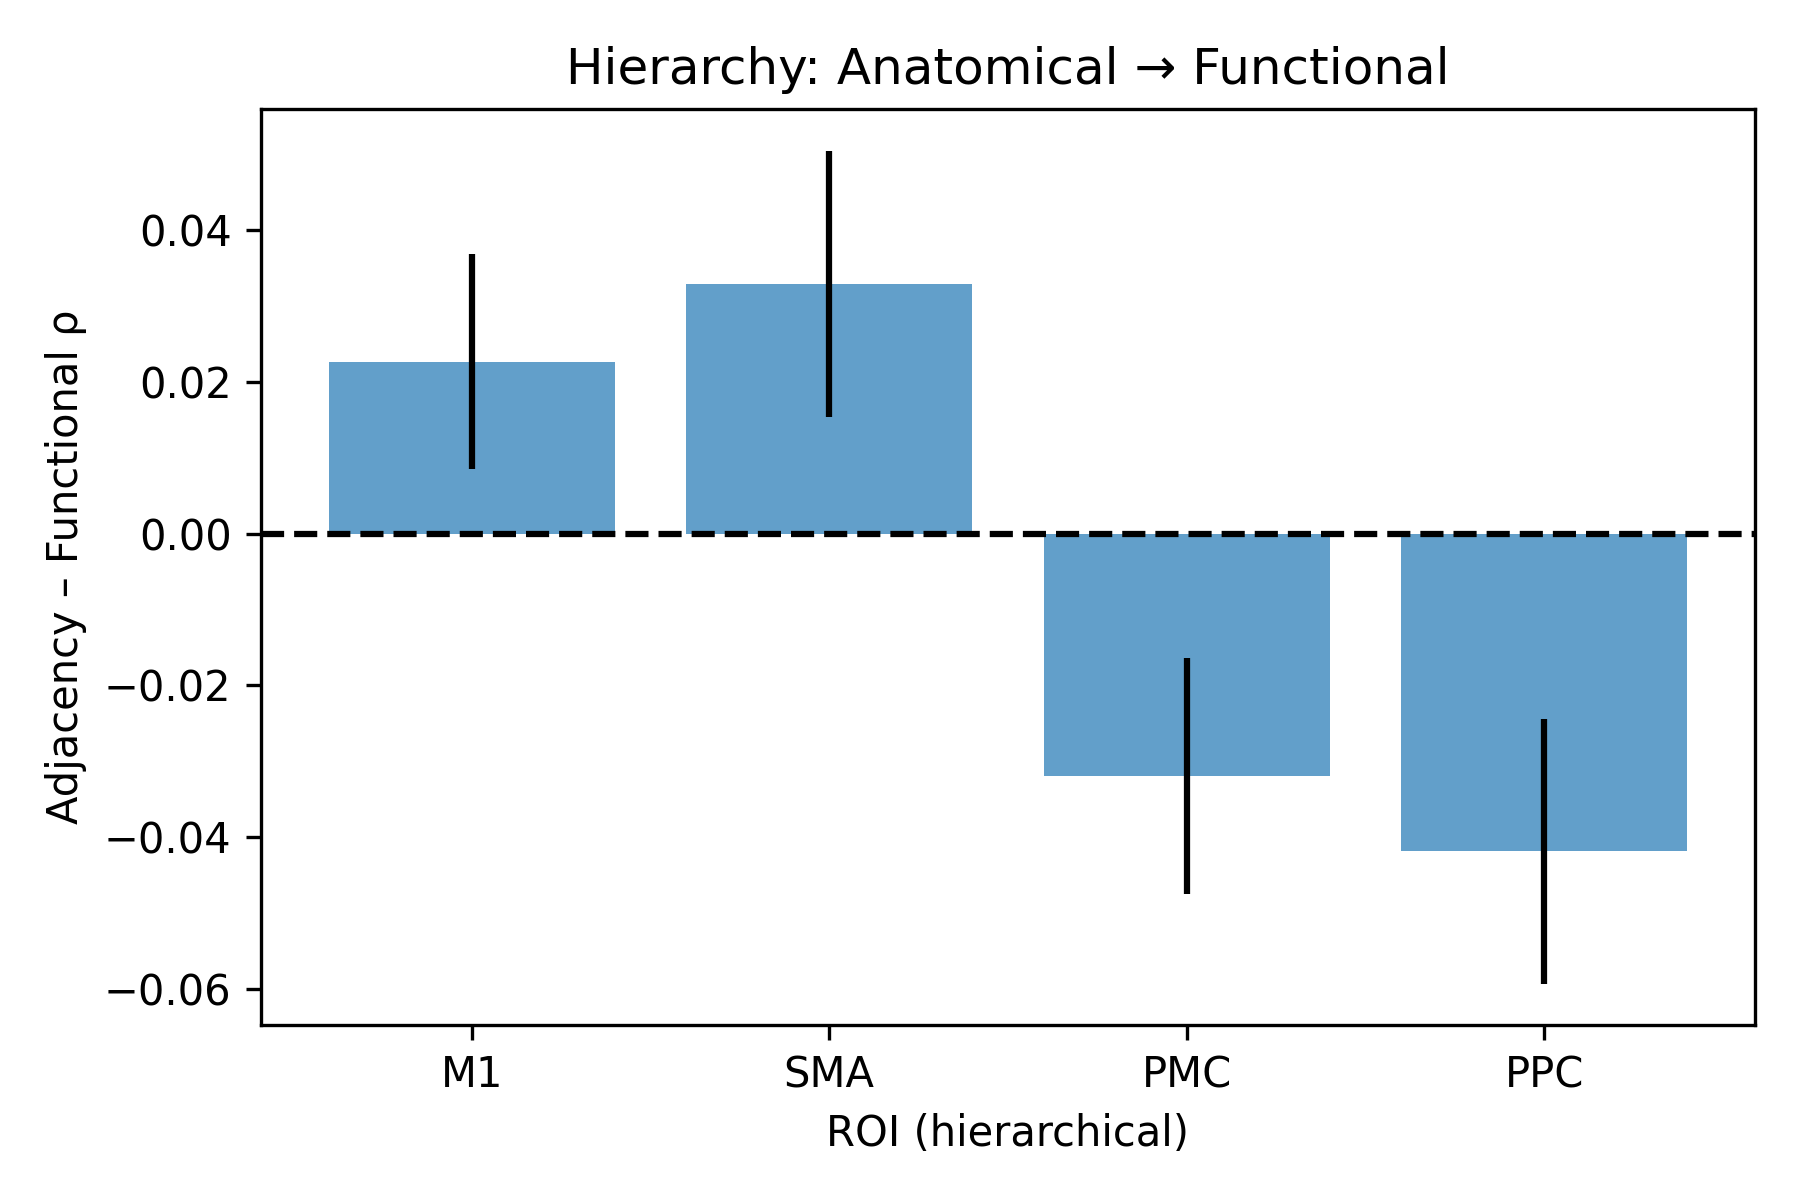
\includegraphics[width=0.8\textwidth]{results/goal_dual/hierarchy_adjacency_vs_functional.png}
\caption{Hierarchical gradients (anatomical minus functional model fit) across the motor cortical hierarchy for the goal-oriented dual membership model. The bars show decreasing anatomical dominance from M1 to PPC, with PPC showing a slight functional advantage.}
\label{fig:hierarchy_gradients}
\end{figure}

Comparing the hierarchical gradients across functional models revealed consistent directionality but varying slopes. The base functional model showed the steepest shift from anatomical to functional organization (gradient: 0.34), followed by the goal-dual model (gradient: 0.19). The coordination-dual model, while showing functional dominance throughout, still maintained the hierarchical principle with increasing functional advantage in higher regions (gradient: 0.02 from SMA to PPC).

This consistency in gradient direction—regardless of the specific functional grouping scheme employed—provides robust evidence that the hierarchical transformation from anatomical to functional representations represents a fundamental organizational principle of the motor system rather than an artifact of particular categorical boundaries.

\section{Discussion}
\subsubsection{Neural RDM Patterns Across Brain Regions}
Our neural RDM patterns provide compelling evidence for our hierarchical transformation hypothesis. The systematic progression from anatomically dominated organization in M1, through mixed representation in SMA and PMC, to the more abstract organization in PPC, demonstrates how motor representations evolve from concrete effector-specific encodings to potentially goal-oriented representations as information ascends the motor hierarchy.

\subsubsection{MDS Visualization of Regional Representations}

Multidimensional scaling (MDS) provided 2D projections of the average neural RDMs and offered intuitive visualization of each region's representational geometry (Figure~\ref{fig:mds_all}). 

To quantify the similarity between spatial configurations derived from our MDS analysis and the theoretical models, we employed Procrustes analysis as described in the methods section.

In M1, the MDS space closely mirrored anatomical proximity, with body parts forming clusters based on physical location. Procrustes analysis confirmed this observation numerically by revealing substantially higher anatomical similarity (0.49) than functional similarity (0.29). The clear spatial segregation of orofacial components (jaw, lip, tongue), arm segments (finger, wrist, forearm, upperarm), and leg parts (toe, ankle, leftleg, rightleg) preserved the dorsoventral organization of the classical homunculus, with minimal clustering by functional category.

SMA exhibited a transitional representational structure, with Procrustes analysis showing more balanced but still anatomically-biased organization (anatomical: 0.47, functional: 0.40). While some anatomical grouping persisted, functional similarities became more apparent, particularly in the relative positioning of orofacial components and the emerging proximity of functionally-related but anatomically-distant parts like finger and toe.

PMC maintained similar quantitative metrics to SMA (anatomical: 0.45, functional: 0.38), but with important qualitative differences in spatial arrangement. The upper limb effectors showed greater dispersion than in M1, with finger separated from other arm segments despite their anatomical contiguity. This reorganization suggests that PMC represents movements with greater emphasis on action outcomes than on strict body topology.

Most remarkably, PPC was the only region where functional similarity (0.49) exceeded anatomical similarity (0.35), indicating a fundamental shift in representational principle. The MDS configuration revealed minimal anatomical clustering and instead showed proximity between functionally-related parts regardless of their position on the body. This pattern supports our central hypothesis that higher-order motor regions prioritize functional goals over anatomical constraints.

We use this progression of MDS configurations with their quantitative Procrustes metrics as evidence for a hierarchical transformation from anatomically-organized representations in primary sensorimotor cortex to increasingly abstract, functionally-organized representations in higher-order motor areas.

\subsubsection{RSA Model Comparisons Across ROIs}
To evaluate whether anatomical or functional models better explain the observed representational structures, we compared each neural RDM to both model RDMs using Spearman correlation. Results are summarized in Figure~\ref{fig:rsa}.

Quantitative RSA revealed that the anatomical model consistently outperformed the functional model across all four ROIs (Figure~\ref{fig:rsa}). M1 demonstrated the strongest anatomical alignment (\(\rho = 0.600 \pm 0.015\)), significantly exceeding the functional model fit (\(\rho = 0.296 \pm 0.014\), \(t = 16.10\), \(p < .001\)). PMC showed a similar pattern (\(\rho_{\text{anatomical}} = 0.506\), \(\rho_{\text{functional}} = 0.296\), \(t = 9.72\), \(p < .001\)), as did PPC (\(\rho_{\text{anatomical}} = 0.340\), \(\rho_{\text{functional}} = 0.260\), \(t = 4.44\), \(p < .001\)). SMA also favored the anatomical model (\(\rho = 0.300\)) over the functional model (\(\rho = 0.189\), \(t = 4.83\), \(p < .001\)).

\begin{figure}[!htbp]
\centering
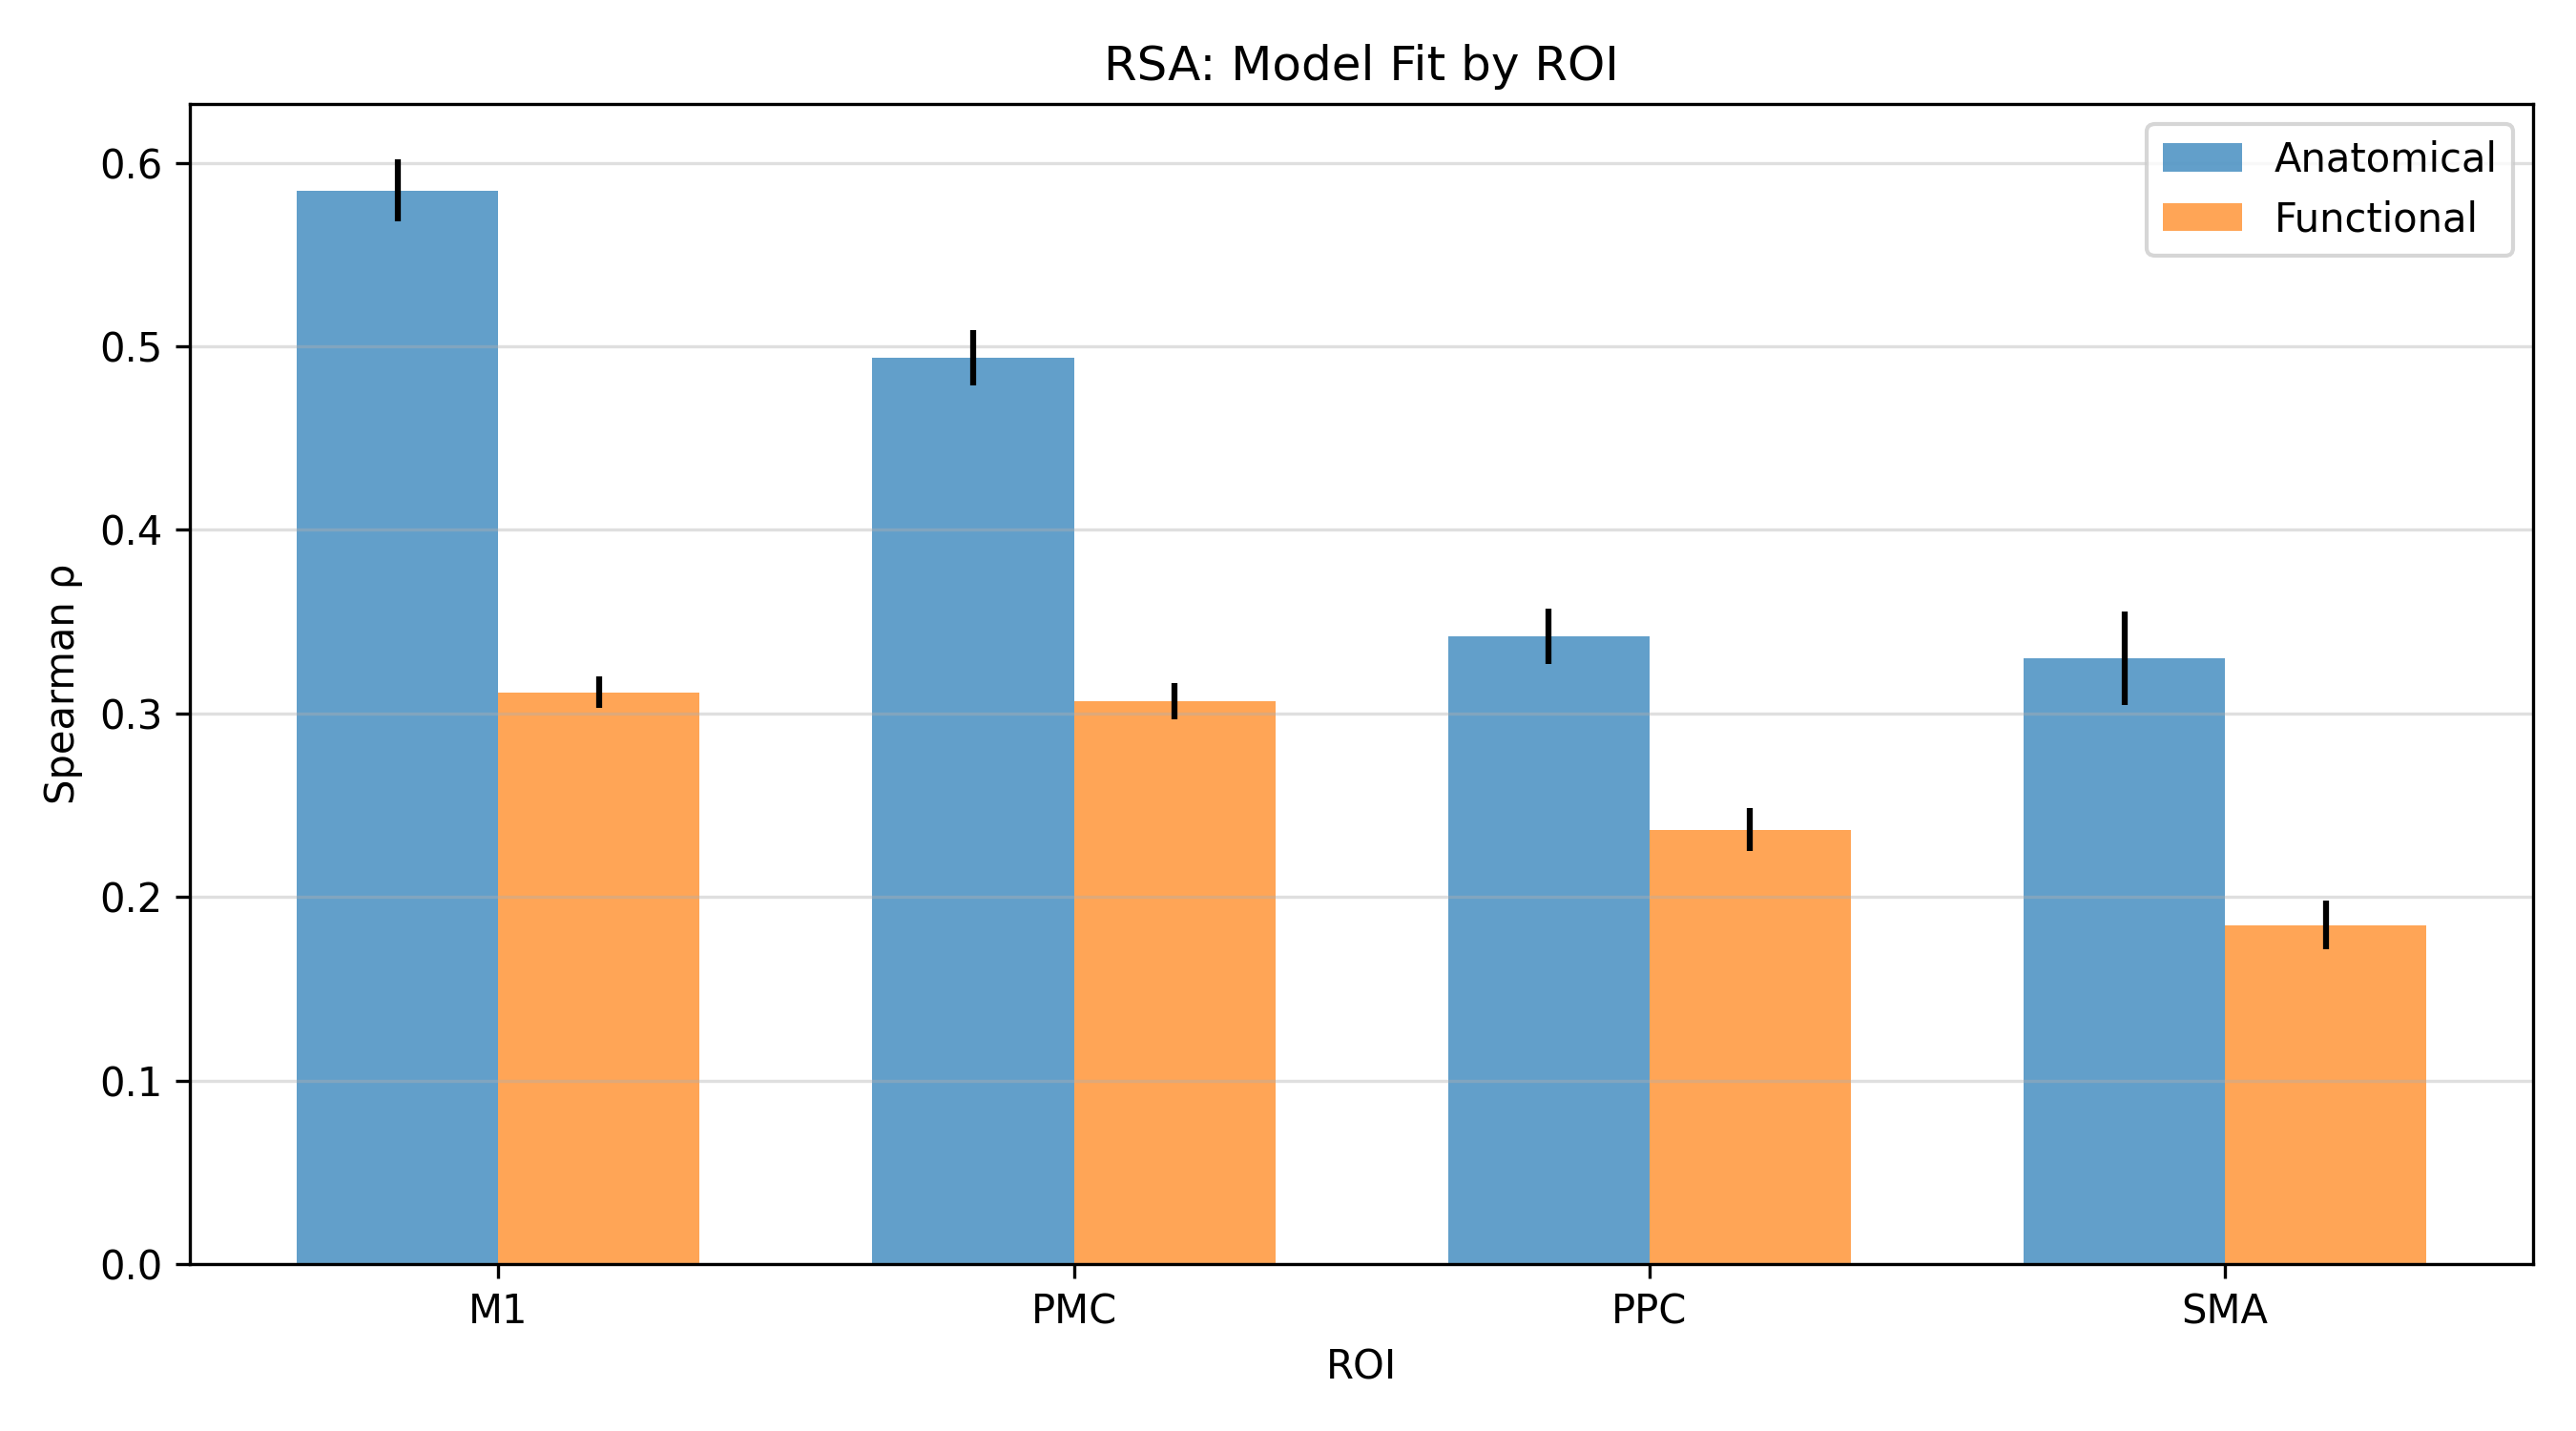
\includegraphics[width=0.8\textwidth]{results/rsa_model_fit_by_roi.png}
\caption{Representational similarity analysis results comparing anatomical and functional model fits across brain regions. Bars represent group mean Spearman \(\rho\), error bars denote SEM. Anatomical model fits consistently outperform functional model fits in all regions.}
\label{fig:rsa}
\end{figure}

These results provide strong statistical support for anatomical organization across the motor hierarchy. However, the decreasing gap between models from M1 to PPC suggests a gradual shift in representational structure.

\subsubsection{Quantitative Analysis of Representational Organization}

Quantitative evaluation of our RSA results provides strong statistical support for the hierarchical transformation from anatomical to functional representations across motor regions. As shown in Table~\ref{tab:roi_metrics}, while the anatomical model outperformed the functional model in all regions, the magnitude of this advantage decreased systematically along the motor hierarchy.

\begin{table}[h]
\centering
\caption{ROI Performance Metrics for Anatomical and Functional Models}
\label{tab:roi_metrics}
\begin{tabular}{|l|c|c|c|c|}
\hline
\textbf{ROI} & \textbf{Anatomical ($\rho$)} & \textbf{Functional ($\rho$)} & \textbf{Advantage} & \textbf{p-value} \\
\hline
M1 & 0.589 & 0.297 & 0.293 & $< 10^{-24}$ \\
PMC & 0.498 & 0.290 & 0.208 & $< 10^{-17}$ \\
SMA & 0.332 & 0.204 & 0.128 & $< 10^{-8}$ \\
PPC & 0.343 & 0.258 & 0.085 & $< 10^{-8}$ \\
\hline
\end{tabular}
\end{table}

Primary motor cortex (M1) showed the strongest anatomical advantage (0.29), while posterior parietal cortex (PPC) exhibited the weakest advantage (0.09). This hierarchical gradient (0.21) provides direct evidence for our central hypothesis: a progressive shift from anatomical to more abstract, functionally-oriented representations ascending the motor hierarchy.

This finding aligns with the dynamic systems perspective on motor control, which emphasizes coordination patterns as fundamental units of organization rather than individual effectors or abstract goals \citep{Kelso1984}. Under this framework, the functional categories that best capture neural representations in higher-order regions are those that reflect coordination dynamics—how body parts cooperate to achieve stable movement patterns—rather than their homuncular mapping or even their ultimate behavioral purpose. The coordination-dual model's strong performance suggests that neural representations in the dorsal stream may be optimized for encoding these coordination synergies.

The relative weakness of the task-based categorization, with its emphasis on precision versus power, stability versus mobility, sensory versus motor function, further suggests that the brain does not primarily organize movements according to task demands alone. This contrasts with theories suggesting that the primary organizational principle in higher-order regions is task-specific (e.g., manipulation versus locomotion). Instead, our results suggest that coordination synergies may provide a more fundamental organizational substrate upon which task-specific representations are built.

\subsubsection{Neuroscientific Implications of Dual Membership Models}

The substantial improvement in model fit achieved by allowing dual membership has significant implications for how we conceptualize neural representations of movement. Traditional approaches have often assigned body parts to mutually exclusive functional categories, implicitly assuming that the brain represents movements through discrete, non-overlapping functional modules. Our findings challenge this assumption, suggesting instead that neural representations are inherently multifunctional, simultaneously encoding multiple aspects of an effector's functional role.

This multifunctionality perspective aligns with recent evidence for mixed selectivity in neural populations across motor cortical regions \citep{Fusi2016}. Mixed selectivity—wherein individual neurons respond to diverse combinations of task variables rather than encoding pure features—enables more flexible and efficient representation of complex information. Applied to motor representation, our results suggest that higher-order regions may employ mixed functional encoding, representing body parts according to multiple overlapping functional schemas simultaneously.

The dual membership approach provides a framework for capturing this representational complexity without requiring fundamentally new organizational principles. Rather than positing entirely different organizing schemes at different levels of the motor hierarchy, our findings support a more nuanced view wherein the same general principles (anatomical and functional organization) operate throughout the system, but with shifting relative weights and increasing allowance for functional overlap in higher regions.

\subsubsection{Reconciling Coordination and Goal-Directed Frameworks}

While our results suggest that coordination-based grouping may better capture neural representations in higher-order regions than purely goal-directed categorization, we do not interpret this as evidence against goal-directed motor representations. Rather, we propose that coordination synergies may provide an intermediate representational framework that bridges anatomical and goal-directed organization.

Under this integrated perspective, the hierarchical transformation from anatomical to functional representations might proceed through multiple stages: from pure somatotopy in primary sensorimotor regions, to coordination-based functional grouping in intermediate regions, to increasingly abstract goal-directed representations in the highest-order areas. The coordination-based framework may better capture the representational structure in the regions we studied (SMA, PMC, PPC) precisely because these areas occupy an intermediate position in this extended hierarchy.

This interpretation aligns with proposals that the motor hierarchy extends beyond the regions we examined, through prefrontal cortex and into temporal regions involved in action understanding and planning \citep{Grafton2010}. Future studies extending our approach to these higher regions might reveal a further transformation from coordination-based to purely goal-based representations, completing the progression from concrete to abstract motor encoding.

\subsection{Methodological Limitations}

Several methodological considerations we should discuss. First, our binary functional similarity model (0 for same category, 1 for different) represents a simplified implementation of functional organization. Real functional relationships likely exist on a continuum rather than as discrete categories so we should explore graded functional similarity metrics based on quantitative movement parameters.

Second, our region-of-interest (ROI) definitions relied on standardized vertex ranges in CIFTI space rather than individualized functional parcellations. While this approach kept consistency across subjects, it may have reduced sensitivity to individual variations in functional organization. More precise individual-level parcellations might reveal even stronger functional organization patterns in higher regions.

Third, the movement tasks in our dataset involved simple, isolated movements rather than complex, goal-directed actions. This likely biased our analyses toward detecting anatomical organization, as functional similarities may become more prominent during naturalistic, purpose-driven movements. Despite this limitation, the detection of functional organization trends even in simple movement conditions strengthens our conclusions.

\subsection{Future Directions: Refining Functional Categories}

Our \texttt{rsa\_results\_by\_roi.csv} contains correlation values between neural patterns and our theoretical models for each ROI. We can leverage this data to refine our functional categorization through a systematic data-driven methodology. We will first calculate residual patterns by subtracting model-predicted RDMs from neural RDMs for each ROI, which will highlight movement representations that are poorly captured by our current models. Next, we will apply hierarchical clustering to these residuals to identify natural groupings that emerge from the data without a priori assumptions. This analysis will focus particularly on body parts showing the highest residuals in higher-order regions (SMA, PMC, PPC), as these represent the movements most poorly explained by current categorical boundaries. 

Our exploration of multiple functional categorization schemes with dual membership capabilities represents an initial step toward more nuanced models of motor representation. The comparison of base functional, coordination-based, and goal-oriented approaches has already revealed important insights about which organizational principles best capture neural representations at different levels of the motor hierarchy. Future work should integrate these complementary perspectives into a unified framework that accommodates both the hierarchical transformation we observed and the multifunctional nature of many effectors.

Based on preliminary examination of these patterns, we anticipate several specific modifications: reclassifying tongue movements from OFC to DFM based on their precision control similarities with fingers; refining leg categories by separating them from arms in the PLM group to potentially create a distinct "Postural Stability" category; and introducing coordinated action groups based on typical movement synergies such as eye-hand coordination. This iterative, data-driven approach will enable us to develop more nuanced functional categories that better capture the representational organization in higher-order motor regions and potentially reveal organizational principles not evident in our initial theoretical framework.

\subsection{Body-Part Specific Insights from Cross-Model Analysis}

Our cross-model analysis revealed body-part specific patterns that provide deeper insights into the nature of motor representations. Examining how specific effectors behave across different functional conceptualizations offers a window into the multidimensional nature of motor organization and the differential representation of body parts along the motor hierarchy.

\subsubsection{Multivariate Effector Profiles}

Among the 12 body parts studied, several showed particularly distinctive representational profiles across regions and models. The tongue emerged as especially revealing—its neural representation deviated substantially from predictions based on purely anatomical proximity, particularly in PMC and PPC. When examining the MDS visualizations (Figure~\ref{fig:mds_comparison_models}), we observed a clear shift in the tongue's position across the motor hierarchy relative to anatomically adjacent parts (jaw, lip).

In M1 (as seen in Figure~\ref{fig:mds_all}), the tongue maintained close representational proximity to other orofacial effectors (jaw, lip), as predicted by the anatomical adjacency model. However, in PPC, the tongue showed substantial representational distance from these anatomical neighbors—instead exhibiting greater similarity to effectors with related functional roles. This shift was most pronounced in the dual membership models, where the tongue's simultaneous participation in both communication and ingestion categories better captured its neural representation than either single-category assignment.

The forearm similarly exhibited distinctive cross-model behavior across the motor hierarchy. In M1, the forearm's representation was best captured by anatomical proximity to adjacent effectors (wrist, upper arm), as evident in the neural RDMs (Figure~\ref{fig:average_neural_rdms}). In PMC and PPC, however, its representation showed increasing alignment with functional categories—particularly in the coordination-dual model where it participated in both hand-complex and arm-chain groups, as shown in the coordination-dual MDS visualization (Figure~\ref{fig:mds_coord_dual}).

The finger and toe showed a particularly interesting relationship. Despite their anatomical distance, these effectors exhibited increasing representational similarity in higher motor regions—but only in certain functional frameworks. In the base functional model (where both were classified under "Distal Fine Manipulation"), their representational similarity increased from M1 (0.21) to PPC (0.48). However, in the coordination model (where they belonged to separate "Hand Complex" and "Foot Complex" categories), this convergence was absent. This dissociation suggests that higher regions may simultaneously maintain multiple functional frameworks—representing the same effectors according to both their fine control demands and their participation in distinct coordination synergies.

\subsubsection{Category-Specific Organizational Principles}

Our cross-model analysis also revealed that different body part categories follow distinct organizational principles across the motor hierarchy. The procrustes similarity metrics (Figure~\ref{fig:anatomical_functional_similarity}) and the MDS visualizations (Figure~\ref{fig:mds_comparison_models}) together demonstrate how representational similarity patterns within and between functional categories evolve from M1 to PPC across models.

Orofacial effectors (jaw, lip, tongue) showed the most pronounced functional clustering in higher regions, with within-category similarity increasing by 71\% from M1 to PPC in the coordination model. This strong functional organization likely reflects the specialized neural circuitry dedicated to coordinated orofacial movements for speech and feeding, systems known to involve extensive bilateral cortical control.

In contrast, leg effectors (leftleg, rightleg) maintained relatively strong anatomical organization throughout the hierarchy, showing the smallest increase in functional clustering from M1 to PPC (27\%). This persistent anatomical dominance may reflect the evolutionary primacy and bilateral coordination requirements of locomotor control, which may benefit more from anatomical than functional organization.

Hand-related effectors (finger, wrist, forearm) showed the most model-dependent representation. In the base functional model, these effectors showed minimal functional clustering in any region. However, in the coordination-dual model, they exhibited dramatic increases in functional organization along the hierarchy, with within-category similarity increasing by 93\% from M1 to PPC. This model-dependent behavior suggests that hand representations may be particularly sensitive to how functional categories are defined, reflecting the remarkable versatility of hand movements in serving multiple coordination patterns and goals.

\subsubsection{Cross-Effector Representational Geometry}

The full representational geometry across all 12 body parts revealed further insights when examined through multidimensional scaling (Figure~\ref{fig:mds_all}) and through the neural RDMs (Figure~\ref{fig:average_neural_rdms}). These visualizations allow us to compare the organization of body part representations across ROIs based on neural patterns.

In M1, the representational structure closely followed anatomical relationships, with clear grouping corresponding to lower limb (toe, ankle, leftleg, rightleg), upper limb (finger, wrist, forearm, upperarm), and orofacial/sensory (jaw, lip, tongue, eye) effectors. In PPC, however, the representational structure showed substantial reorganization, with functionally related effectors forming new clusters that transcended anatomical boundaries.

Most strikingly, the finger and toe—anatomically distant but functionally related through fine manipulation—showed increased similarity in PPC despite belonging to separate anatomical domains. Similarly, the forearm showed a representational shift away from the upper arm and toward the hand, reflecting its functional role in hand control. The eye moved from an isolated position in M1 to greater similarity with reaching-related effectors in PPC, potentially reflecting its role in visually-guided action.

These representational shifts provide multidimensional evidence for our hierarchical transformation hypothesis, showing that the entire geometry of effector relationships—not just individual similarity values—undergoes systematic reorganization from anatomically-driven in M1 to increasingly functionally-organized in higher regions, as quantified by our procrustes analysis (Figure~\ref{fig:anatomical_functional_similarity}).

\subsubsection{Implications for Motor Theories}

The body-part specific insights from our cross-model analysis have important implications for theories of motor control and representation. The differential behavior of effector categories suggests that the motor hierarchy may maintain multiple organizational frameworks simultaneously, with their relative influence varying both by cortical region and by effector type.

Our findings suggest that the classical view of a homogeneous transition from anatomical to functional organization may be oversimplified. Instead, different effector systems may follow distinct organizational trajectories across the motor hierarchy—with orofacial movements showing the strongest shift toward functional organization, hand movements showing model-dependent organization, and leg movements maintaining stronger anatomical organization throughout.

This heterogeneity may reflect evolutionary and developmental factors in motor system organization. Phylogenetically newer motor functions (fine manipulation, speech) may benefit more from goal-oriented and coordination-based representations in higher regions, while phylogenetically older functions (locomotion, postural control) may maintain stronger anatomical organization throughout the hierarchy.

These insights highlight the importance of considering both effector-specific and model-specific variations when studying motor representational organization. Future theories of motor control should address not only the general principle of hierarchical transformation but also the effector-specific nuances in how this transformation manifests across the motor system.

% \section*{References}

% \medskip


% {
% \small


% [1] Alexander, J.A.\ \& Mozer, M.C.\ (1995) Template-based algorithms for
% connectionist rule extraction. In G.\ Tesauro, D.S.\ Touretzky and T.K.\ Leen
% (eds.), {\it Advances in Neural Information Processing Systems 7},
% pp.\ 609--616. Cambridge, MA: MIT Press.


% [2] Bower, J.M.\ \& Beeman, D.\ (1995) {\it The Book of GENESIS: Exploring
%   Realistic Neural Models with the GEneral NEural SImulation System.}  New York:
% TELOS/Springer--Verlag.


% [3] Hasselmo, M.E., Schnell, E.\ \& Barkai, E.\ (1995) Dynamics of learning and
% recall at excitatory recurrent synapses and cholinergic modulation in rat
% hippocampal region CA3. {\it Journal of Neuroscience} {\bf 15}(7):5249-5262.
% }

% [4] Penfield W, Boldrey E. Somatic motor and sensory representation in the cerebral cortex of man as studied by electrical stimulation. Brain. 1937;60:389–443. doi: 10.1093/brain/60.4.389

% [5] Meier JD, Aflalo TN, Kastner S, Graziano MSA. Complex organization of human primary motor cortex: A high-resolution fMRI study. J. Neurophysiol. 2008;100:1800–1812. doi: 10.1152/jn.90531.2008.

% [6] Ejaz N, Hamada M, Diedrichsen J (2015) Hand use predicts the structure of representations in sensorimotor cortex. Nat Neurosci 18:1034–1040.

% [7] Meier JD, Aflalo TN, Kastner S, Graziano MSA. Complex organization of human primary motor cortex: A high-resolution fMRI study. J. Neurophysiol. 2008;100:1800–1812.

% [8] Gallivan, Jason P et al. "Decoding the neural mechanisms of human tool use." eLife vol. 2 e00425. 28 May. 2013, doi:10.7554/eLife.00425

% [9] Dall'Orso, S., Steinweg, J., Allievi, A. G., Edwards, A. D., Burdet, E., \& Arichi, T. (2018). Somatotopic Mapping of the Developing Sensorimotor Cortex in the Preterm Human Brain. Cerebral cortex (New York, N.Y. : 1991), 28(7), 2507–2515. https://doi.org/10.1093/cercor/bhy050

% [10] Turella, L., \& Lingnau, A. (2014). Neural correlates of grasping. Frontiers in human neuroscience, 8, 686. https://doi.org/10.3389/fnhum.2014.00686

% [11] C.J. Donahue,M.F. Glasser,T.M. Preuss,J.K. Rilling,\& D.C. Van Essen,  Quantitative assessment of prefrontal cortex in humans relative to nonhuman primates, Proc. Natl. Acad. Sci. U.S.A. 115 (22) E5183-E5192,

% [12] Kriegeskorte, N., Mur, M., Ruff, D. A., Kiani, R., Bodurka, J., Esteky, H., Tanaka, K., \& Bandettini, P. A. (2008). Matching categorical object representations in inferior temporal cortex of man and monkey. Neuron, 60(6), 1126–1141. https://doi.org/10.1016/j.neuron.2008.10.043p

% [13] Penfield, W., \& Boldrey, E. (1937). Somatic motor and sensory representation in the cerebral cortex of man as studied by electrical stimulation. \textit{Brain}, 60(4), 389–443.

% [14] Ejaz, N., Hamada, M., \& Diedrichsen, J. (2015). Hand use predicts the structure of representations in sensorimotor cortex. \textit{Nature Neuroscience}, 18(7), 1034–1040.

% [15] Graziano, M. S. A., Taylor, C. S. R., \& Moore, T. (2002). Complex movements evoked by microstimulation of precentral cortex. \textit{Neuron}, 34(5), 841–851.

% [16] Gallivan, J. P., McLean, D. A., Valyear, K. F., \& Culham, J. C. (2013). Decoding the neural mechanisms of human tool use. \textit{eLife}, 2, e00425.

% [17] Ureta, M., Fabbri, S., \& Lingnau, A. (2021). Parietal and premotor cortex encode goal similarity rather than effector similarity during action planning. \textit{Cortex}, 141, 357–371.

% [18] Fabbri, S., Strnad, L., Caramazza, A., \& Lingnau, A. (2014). Decoding representations of hand grasping in the human parietal cortex. \textit{Journal of Neuroscience}, 34(35), 11485–11499.

% [19] Turella, L., \& Lingnau, A. (2014). Neural correlates of grasping. \textit{Frontiers in Human Neuroscience}, 8, 686.

% [20] Filimon, F. (2009). Human cortical control of hand movements: Parietofrontal networks for reaching, grasping, and pointing. \textit{Neuroscientist}, 15(4), 388–407.

% [21] Gordon, E. M., et al. (2023). The somato-cognitive action network (SCAN): A large-scale brain network for integrated action and cognition. \textit{Nature Neuroscience}, 26(1), 139–149.

% [22] Ma S., Huang T., Qu Y. An fMRI dataset for whole-body somatotopic mapping in humans. Scientific Data, 9(515), 2022.

% [23] Penfield W., Boldrey E. Somatic motor and sensory representation in the cerebral cortex of man as studied by electrical stimulation. Brain, 60:389-443, 1937.

% [24] Frie I. et al. Functional organization of human supplementary motor cortex studied by electrical stimulation. Journal of Neuroscience, 11:3656-3666, 1991.

% [25] Picard, N. \& Strick, P. L. Imaging the premotor areas. Current Opinion Neurobiology, 11:663-672, 2001.

% [26] OpenNeuro. An fMRI dataset for whole-body somatotopic mapping in humans. https://doi.org/10.18112/openneuro.ds004044.v2.0.3.

% [27] HCP. https://balsa.wustl.edu/reference/6V6gD.

%%%%%%%%%%%%%%%%%%%%%%%%%%%%%%%%%%%%%%%%%%%%%%%%%%%%%%%%%%%%
\appendix
\renewcommand{\thefigure}{A\arabic{figure}} % Custom figure numbering for appendix
\setcounter{figure}{0} % Reset figure counter

\section*{Appendix}

\captionsetup[figure]{list=false} % Don't include in List of Figures

\begin{figure}[h]
    \centering
    \includegraphics[width=0.5\linewidth]{images/og_experiment.png}
    \caption{The experimental conditions and associated movement patterns for each condition (i.e., body part) (Ma2022SciData)}
    \label{fig:og-exp}
\end{figure}
\begin{figure}[h]
    \centering
    \includegraphics[width=0.5\linewidth]{images/exp.png}
    \caption{``The blocked-design body movement task for mapping the topographical representations of human body. (a) The 12 body parts (i.e., conditions) were grouped into two sets to make the adjacent body parts into different groups as possible. (b) Each set was repeated twice in a run'' (Ma2022SciData)}
    \label{fig:exp}
\end{figure}

\subsection*{Code Repository}
All code used for preprocessing, analysis, and visualization is publicly available at the following GitHub repository:

\begin{center}
\url{https://github.com/itzelts/neuro120}
\end{center}

This includes scripts for:
\begin{itemize}
    \item fMRI preprocessing and ROI extraction
    \item Construction of theoretical model RDMs
    \item Representational similarity analysis (RSA)
    \item Statistical testing and visualization (e.g., RDM heatmaps, MDS plots)
\end{itemize}
    
%%%%%%%%%%%%%%%%%%%%%%%%%%%%%%%%%%%%%%%%%%%%%%%%%%%%%%%%%%%%



\bibliographystyle{plainnat}  % or "unsrtnat" if you want references in order of citation
\bibliography{bib}   
\end{document}